\RCS$Revision: 326816 $
\RCS$HeadURL: svn+ssh://svn.cern.ch/reps/tdr2/papers/SUS-15-005/trunk/SUS-15-005.tex $
\RCS$Id: SUS-15-005.tex 326816 2016-02-19 20:36:18Z sakuma $

\cmsNoteHeader{SUS-15-005\_suppl}

\title{Search for new physics in final states with jets and missing
  transverse momentum in $\sqrt{s}$ = 13 TeV pp collisions with the
  $\alpha_{\text{T}}$ variable. {\it Supplementary material.}}

\address[cern]{CERN}
\author[cern]{The CMS Collaboration}

\date{\today}

\abstract{An inclusive search for supersymmetric processes that
  produce final states with jets and missing transverse momentum is
  performed in pp collisions at a centre-of-mass energy of 13 TeV. A
  dimensionless kinematic variable, $\alpha_{\text{T}}$, is used to
  discriminate between events with genuine and misreconstructed
  missing transverse momentum. A data sample corresponding to an
  integrated luminosity of $2.3~\text{fb}^{-1}$, recorded by the CMS
  experiment at the LHC, is analysed. The observed signal candidate
  event counts are found to be in agreement with the expected
  contributions from standard model processes and the result is
  interpreted in the mass parameter space of supersymmetric simplified
  models.}

\hypersetup{ pdfauthor={Mark Baber, Robert Bainbridge, Freya Blekman,
    Oliver Buchmueller, Jim Brooke, Stefano Casasso, Matthew Citron,
    Adam Elwood, Henning Flaecher, Aran Garcia-Bellido, Christian
    Laner, Kin Ho Lo, Sarah Alam Malik, Bjoern Penning, Tai Sakuma,
    Dominic Smith, Alex Tapper},
  pdftitle={Search for new physics in final states with jets and
    missing transverse momentum in 13 TeV pp collisions with the
    AlphaT variable}, 
  pdfsubject={CMS}, 
  pdfkeywords={CMS, jets, missing transverse momentum, supersymmetry,
    dark matter, AlphaT}, 
}

\newcommand{\kfactor}{\ensuremath{k\text{-factor}}\xspace}
\newcommand{\kfactors}{\ensuremath{k\text{-factors}}\xspace}
\newcommand{\njet}{\ensuremath{n_{\text{jet}}}\xspace}
\newcommand{\njetlow}{\ensuremath{2 \leq \njet \leq 3}\xspace}
\newcommand{\njethigh}{\ensuremath{\njet \geq 4}\xspace}
\newcommand{\nb}{\ensuremath{n_{\text{b}}}\xspace}
\newcommand{\alphat}{\ensuremath{\alpha_{\text{T}}}\xspace}
\newcommand{\alphatcut}{\ensuremath{\alpha_{\text{T}}^{\text{cut}}}\xspace}
\newcommand{\htalphat}{\texttt{HT\_AlphaT}\xspace}
\newcommand{\photon}{\texttt{Photon}\xspace}
\newcommand{\muht}{\texttt{Mu\_HT}\xspace}
\newcommand{\httrigger}{\texttt{HT}\xspace}
\newcommand{\mt}{\ensuremath{M_{\textrm T}}\xspace}
\newcommand{\gj}{\ensuremath{\gamma} + jets\xspace}
\newcommand{\mj}{\ensuremath{\mu} + jets\xspace}
\newcommand{\mmj}{\ensuremath{\mu\mu} + jets\xspace}
\newcommand{\npre}{\ensuremath{N_{\textrm{pred}}}\xspace}
\newcommand{\nobs}{\ensuremath{N_{\textrm{obs}}}\xspace}
\newcommand{\njets}{\ensuremath{N_{\textrm{jet}}}\xspace}
\newcommand{\sq}{\ensuremath{\tilde{\rm q}}\xspace}
\newcommand{\st}{\ensuremath{\tilde{\rm t}}\xspace}
\newcommand{\gl}{\ensuremath{\tilde{\rm g}}\xspace}
\newcommand{\dht}{\ensuremath{\Delta\scalht}\xspace}
\newcommand{\ewk}{\ensuremath{\mathrm{EWK}}\xspace}
\newcommand{\qcd}{\ensuremath{\mathrm{QCD}}\xspace}
\newcommand{\fZinv}[1]{\ensuremath{f_{\rm Zinv}^{#1}}\xspace}
\newcommand{\zInv}[1]{\ensuremath{Z_{\rm inv}^{#1}}\xspace}
\newcommand{\meanHt}[1]{\ensuremath{\langle \HT \rangle^{#1}}\xspace}
\newcommand{\lk}[2]{\ensuremath{L^{\rm #1}_{\rm #2}}\xspace}
\newcommand{\sep}{\ensuremath{68^{\mathrm{th}}}\xspace}
\newcommand{\partonht}{\ensuremath{\scalht^{\rm parton}}\xspace}
\newcommand{\meff}{\ensuremath{M_{\rm eff}}\xspace}
\newcommand{\mhttt}{\ensuremath{\hslash_{\rm T}^{TT}}\xspace}


\newcommand\rs{\raisebox{1.0ex}[-1.0ex]}
\newcommand{\ra}{\ensuremath{\rightarrow}}
\newcommand{\znunu}{\ensuremath{{\text Z} \ra \nu\bar{\nu}}\xspace}
\newcommand{\zll}{\ensuremath{{\text Z} \ra \ell\ell}\xspace}
\newcommand{\zmumu}{\ensuremath{{\text Z} \ra \mu\mu}\xspace}
\newcommand{\zee}{\ensuremath{{\text Z} \ra ee}\xspace}
\newcommand{\wmunu}{\ensuremath{{\text W} \ra \mu\nu}}
\newcommand{\wtaunu}{\ensuremath{{\text W} \ra \tau\nu}}
\newcommand{\dphi}{\ensuremath{\Delta \phi}}
\newcommand{\dphijj}{\ensuremath{\Delta \phi_{ j1,j2}}}
\newcommand{\Pt}{\ensuremath{{p_{\text T}}}\xspace}
\newcommand{\pts}{\ensuremath{p_{\text T}{\text s}}\xspace}
\newcommand{\Et}{\ensuremath{{E_{\text T}}}\xspace}
\newcommand{\ptjf}{\ensuremath{p_{\rm T}^{ {\rm j}_1} }}
\newcommand{\ptjs}{\ensuremath{p_{\rm T}^{ {\rm j}_2} }}
\newcommand{\ptjt}{\ensuremath{p_{\rm T}^{ {\rm j}_3} }}
\newcommand{\etajf}{\ensuremath{\eta^{ {\rm j}_1} }}
\newcommand{\etajs}{\ensuremath{\eta^{ {\rm j}_2} }}
\newcommand{\etajt}{\ensuremath{\eta^{ {\rm j}_3} }}
\newcommand{\ttj}{\ensuremath{\rm{t}\bar{\rm{t}} + jets}\xspace}
\newcommand{\wj}{\ensuremath{\rm W + \textrm{jets}}\xspace}
\newcommand{\wej}{\ensuremath{{\rm W}(\rightarrow{\rm e}\nu) + \textrm{jets}}\xspace}
\newcommand{\wmj}{\ensuremath{{\rm W}(\rightarrow\mu\nu) + \textrm{jets}}\xspace}
\newcommand{\zj}{\ensuremath{{\rm Z} + \textrm{jets}}\xspace}
\newcommand{\zmmj}{\ensuremath{{\rm Z}(\rightarrow\mu\mu) + \textrm{jets}}\xspace}
\newcommand{\zeej}{\ensuremath{{\rm Z}(\rightarrow{\rm ee}) + \textrm{jets}}\xspace}

\newcommand{\al}{\ensuremath{\alpha}}
\newcommand{\alt}{\ensuremath{\alpha_{\text{T}}}\xspace}
\newcommand{\etaabs}{\ensuremath{|\eta|}}
%\newcommand{\gev}{\ensuremath{\mathrm{\,Ge\kern -0.1em V}}}
\newcommand{\pb}{\ensuremath{pb^{-1}}}
\newcommand{\mjj}{\ensuremath{M_{\text{inv}}^{j1,j2}}}
%\newcommand{\ttbar}{\ensuremath{t\bar{t}}}
\newcommand{\chiznew}{\ensuremath{\chi^{0}}\xspace}
\newcommand{\chipnew}{\ensuremath{\chi^{+}}\xspace}
\newcommand{\sQuanew}{\ensuremath{\tilde{\rm q}}\xspace}
\newcommand{\sGlunew}{\ensuremath{\tilde{\rm g}}\xspace}
\newcommand{\ttNew}{\ensuremath{\rm{t}\bar{\rm{t}}}\xspace}
\newcommand{\tev}{\TeV}
%<TW date="30/10/2010">
%\newcommand{\Et}{E_{T}}
\newcommand{\combIso}{Iso_{\textrm{comb.}}}
\renewcommand{\arraystretch}{1.2}
\newcommand{\bigNum}[2]{#1 \, \times \, 10 \, ^{#2}}
%</TW>

\newcommand{\raT}{\ensuremath{R_{\alt}}}
\newcommand{\RaT}{\ensuremath{R_{\alt}}\xspace}

\newcommand{\Ttwocc}{\ensuremath{\text{pp}\,\ra\,\sTop\sTop^{*}\,\ra\,\text{c}\chiz\,\bar{\text{c}}\chiz}}
\newcommand{\Ttwodegen}{\ensuremath{\text{pp}\,\ra\,\sTop\sTop^{*}\,\ra\,\text{b}ff'\chiz \,\text{b}ff'\chiz}}
\newcommand{\Ttwobw}{\ensuremath{\text{pp}\,\ra\,\sTop\sTop^{*}\,\ra\,\text{b}W\chiz \,\bar{\text{b}}W\chiz}}
\newcommand{\Ttwott}{\ensuremath{\text{pp}\,\ra\,\sTop\sTop^{*}\,\ra\,\text{t}\chiz\,\bar{\text{t}}\chiz}}
\newcommand{\Ttwobb}{\ensuremath{\text{pp}\,\ra\,\sBot\sBot^{*}\,\ra\,\text{b}\chiz\,\bar{\text{b}}\chiz}}
\newcommand{\Ttwoqq}{\ensuremath{\text{pp}\,\ra\,\sQua\sQua^{*}\,\ra\,\text{q}\chiz\,\bar{\text{q}}\chiz}}
\newcommand{\Tonebbbb}{\ensuremath{\text{pp}\,\ra\,\sGlunew\sGlunew^{*}\,\ra\,\bar{\text{b}}\text{b}\chiz\,\bar{\text{b}}\text{b}\chiz}}
\newcommand{\Toneqqqq}{\ensuremath{\text{pp}\,\ra\,\sGlunew\sGlunew^{*}\,\ra\,\bar{\text{q}}\text{q}\chiz\,\bar{\text{q}}\text{q}\chiz}}
\newcommand{\Tonetttt}{\ensuremath{\text{pp}\,\ra\,\sGlunew\sGlunew^{*}\,\ra\,\bar{\text{t}}\text{t}\chiz\,\bar{\text{t}}\text{t}\chiz}}

\newcommand\T{\rule{0pt}{2.6ex}}
\newcommand\B{\rule[-1.2ex]{0pt}{0pt}}

\def\eslash{{\hbox{$E$\kern-0.6em\lower-.05ex\hbox{/}\kern0.10em}}}
\def\vecmet{\mbox{$\vec{\eslash}_T$}} %missing ET vector
\def\vecet{\mbox{$\vec{E}_\text{T}$}} % ET vector
\def\MET{\mbox{$\eslash_\text{T}$}\xspace}
%\def\met{\mbox{$\eslash_\text{T}$}\xspace}
\def\met{\mbox{$E_\text{T}^{\rm miss}$}\xspace}
\def\pfmet{\mbox{$\eslash_\text{T}^{\rm PF}$}\xspace}
\def\mex{\mbox{$\eslash_\text{x}$}} %missing Ex
\def\mey{\mbox{$\eslash_\text{y}$}} %missing Ey
\def\mepar{\mbox{$\eslash_\parallel$}}
\def\meperp{\mbox{$\eslash_\perp$}}
\def\Zmm{Z \rightarrow \mu\mu}
\def\metvec{\mbox{$\vec{\met}$}\xspace}
\def\metvecrec{\mbox{$\vec{\met}^{\rm rec}$}\xspace}
\def\metvecgen{\mbox{$\vec{\met}^{\rm gen}$}\xspace}
\def\metgen{\mbox{$\met^{\rm gen}$}\xspace}
\def\metparl{\mbox{$\mepar^{\rm rec}$}\xspace}
\def\metperp{\mbox{$\meperp^{\rm rec}$}\xspace}
\def\deltamet{\mbox{$\Delta\met$}\xspace}
\def\pthat{\mbox{$\hat{p}_T$}\xspace}
\def\hslash{{\hbox{$H$\kern-0.8em\lower-.05ex\hbox{/}\kern0.10em}}}
\def\MHT{\mbox{$\hslash_\text{T}$}\xspace}
%\def\mht{\mbox{$\hslash_\text{T}$}\xspace}
\def\mht{\mbox{$H_{\rm T}^{\rm miss}$}\xspace}
\def\mhtvec{\mbox{$\vec{H}_{\rm T}^{\rm miss}$}\xspace}
%\def\mhtmet{\mbox{$\hslash_\text{T} / \eslash_\text{T}$}\xspace}
\def\mhtmet{\mbox{$\mht / \met$}\xspace}
\def\mhtmetmiss{\mbox{$\H_\text{T}^{\rm miss} / \E_\text{T}^{\rm miss}$}\xspace}
%\def\rmhtmet{\mbox{$R_{\hslash_\text{T} / \eslash_\text{T}}$}\xspace}
\def\rmhtmet{\mbox{$R_{\mht / \met}$}\xspace}
\def\sumet{\mbox{$\sum \rm{E}_\text{T}$}\xspace}
\def\scalht{\mbox{$H_\text{T}$}\xspace}
\def\etmiss{\mbox{$\eslash_\text{T}$}\xspace}
\def\htmiss{\mbox{$\hslash_\text{T}$}\xspace}
\def\mtt{\mbox{$\rm{M}_\text{T2}$}\xspace}
\def\rmec{\mbox{$R_{\mht/\met}$}\xspace}
\def\bdphi{\mbox{$\Delta\phi^{*}_{\rm min}$}\xspace}
\def\dphimhtj{\mbox{$\Delta\phi(j_{1234}, \mht)_{\rm min}$}\xspace}
\def\bigeslash{{\hbox{$E$\kern-0.38em\lower-.05ex\hbox{/}\kern0.10em}}}
\def\bigmet{\mbox{$\bigeslash_T$}}
\def\bighslash{{\hbox{$H$\kern-0.6em\lower-.05ex\hbox{/}\kern0.10em}}}
\def\bigmht{\mbox{$\bighslash_T$}}
\def\incl{\includegraphics[width=0.49\linewidth]}
\def\inclrot{\includegraphics[angle=90,width=0.47\linewidth]}
\def\INCL{\includegraphics[angle=90,width=0.45\linewidth]}
\def\Incl{\includegraphics[angle=90,width=0.60\linewidth]}
\def\cls{\mbox{CL$_s$}\xspace}
\def\nj{\ensuremath{n_{\mathrm{jet}}}}
\def\nb{\ensuremath{n_{\mathrm{b}}}}

\newcommand{\zero}{\ensuremath{\phantom{0}}}


\newlength\cmsFigWidth
\ifthenelse{\boolean{cms@external}}{\setlength\cmsFigWidth{0.85\columnwidth}}{\setlength\cmsFigWidth{0.4\textwidth}}
\ifthenelse{\boolean{cms@external}}{\providecommand{\cmsLeft}{top\xspace}}{\providecommand{\cmsLeft}{left\xspace}}
\ifthenelse{\boolean{cms@external}}{\providecommand{\cmsRight}{bottom\xspace}}{\providecommand{\cmsRight}{right\xspace}}

\maketitle


\clearpage
\begin{figure}[tbhp]
    \caption{ 
    Distributions of data and MC predictions for \scalht (top left), \mht (top right), \nj (bottom left) and \nb (bottom right) 
    for the $\mu+\mathrm{jets}$ control region. 
    It should be kept in mind that the analysis doesn't rely directly on simulation to derive the backgrounds, 
    so these plots are meant to show the shape of some of the variables used in the analysis despite the limitations 
    of the MC modelling. 
    \label{fig:data-MC_plots_SingleMu} }
  \begin{center}
     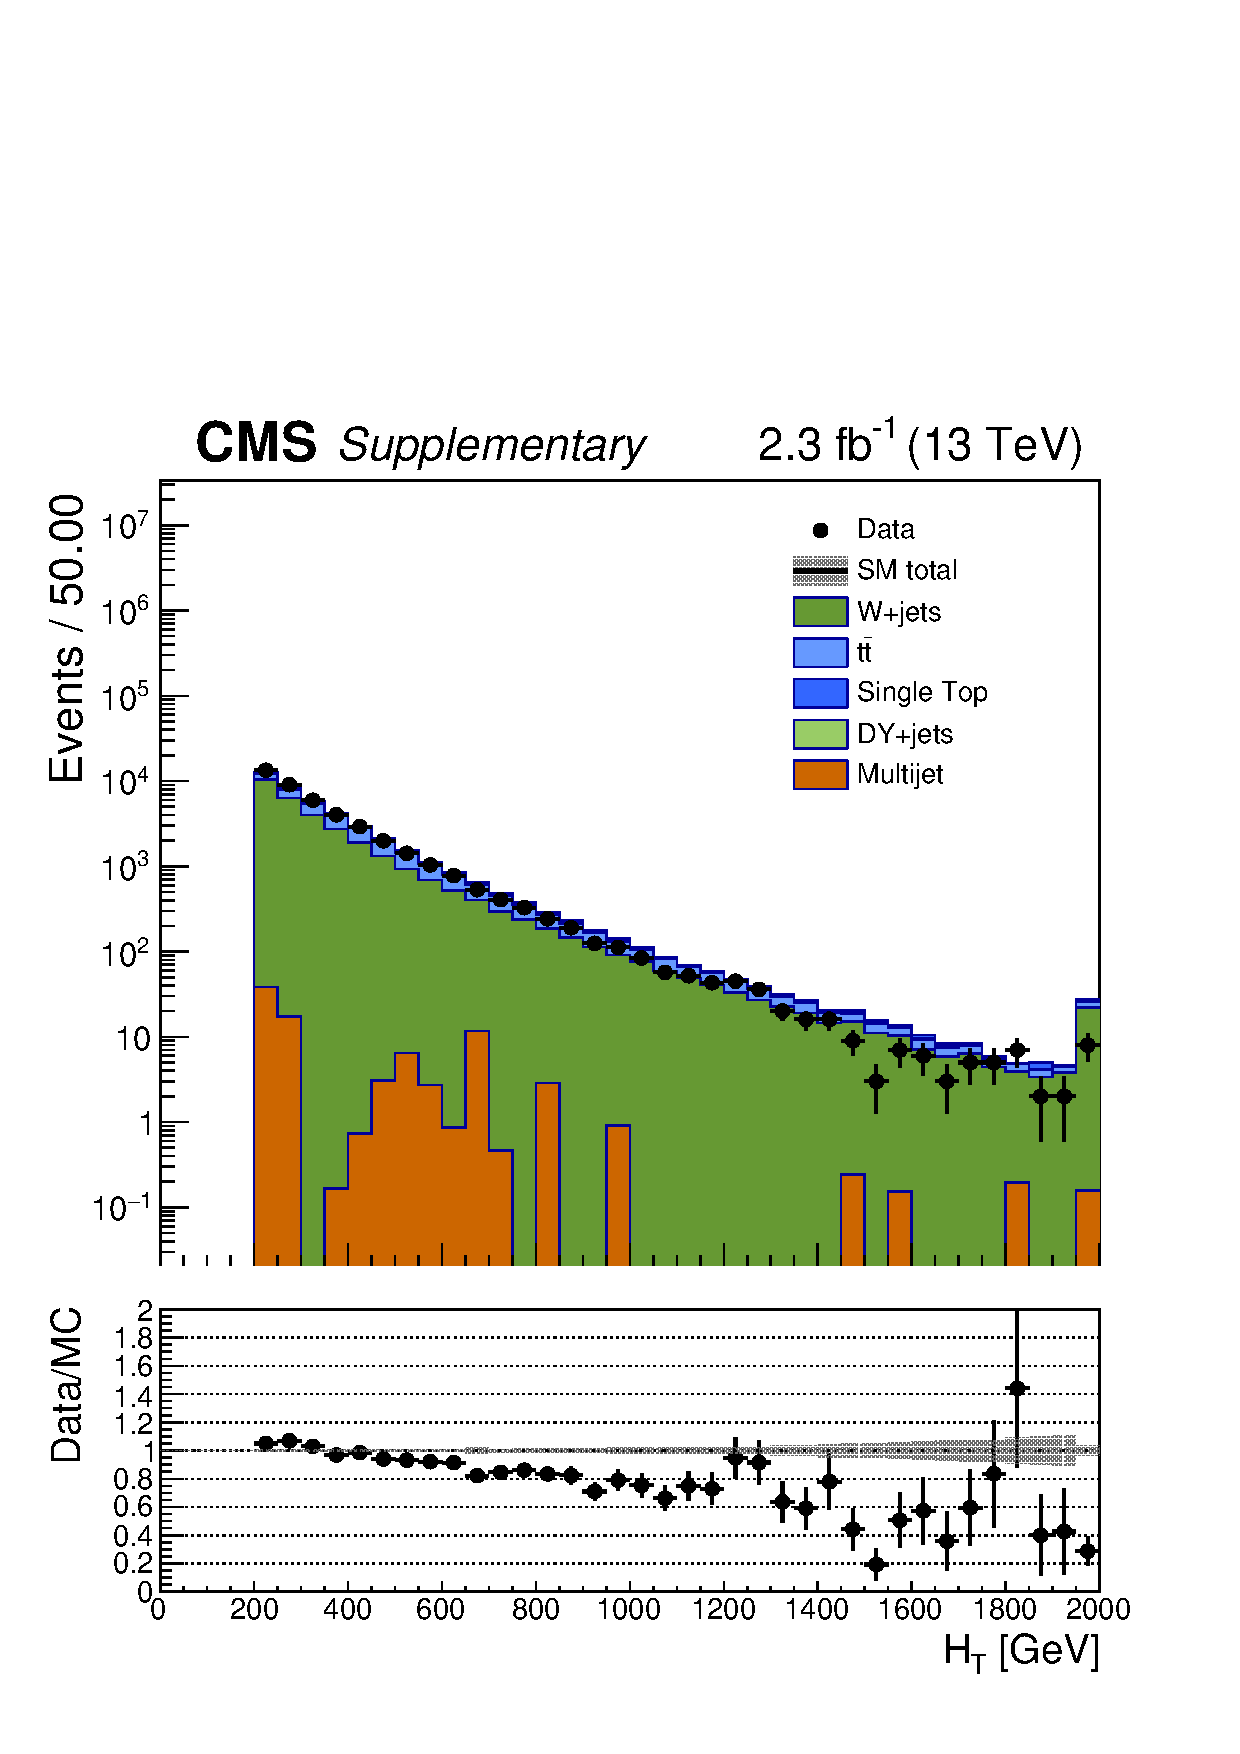
\includegraphics[width=0.45\textwidth]{figures/SingleMu_ht40_all_all} ~~
     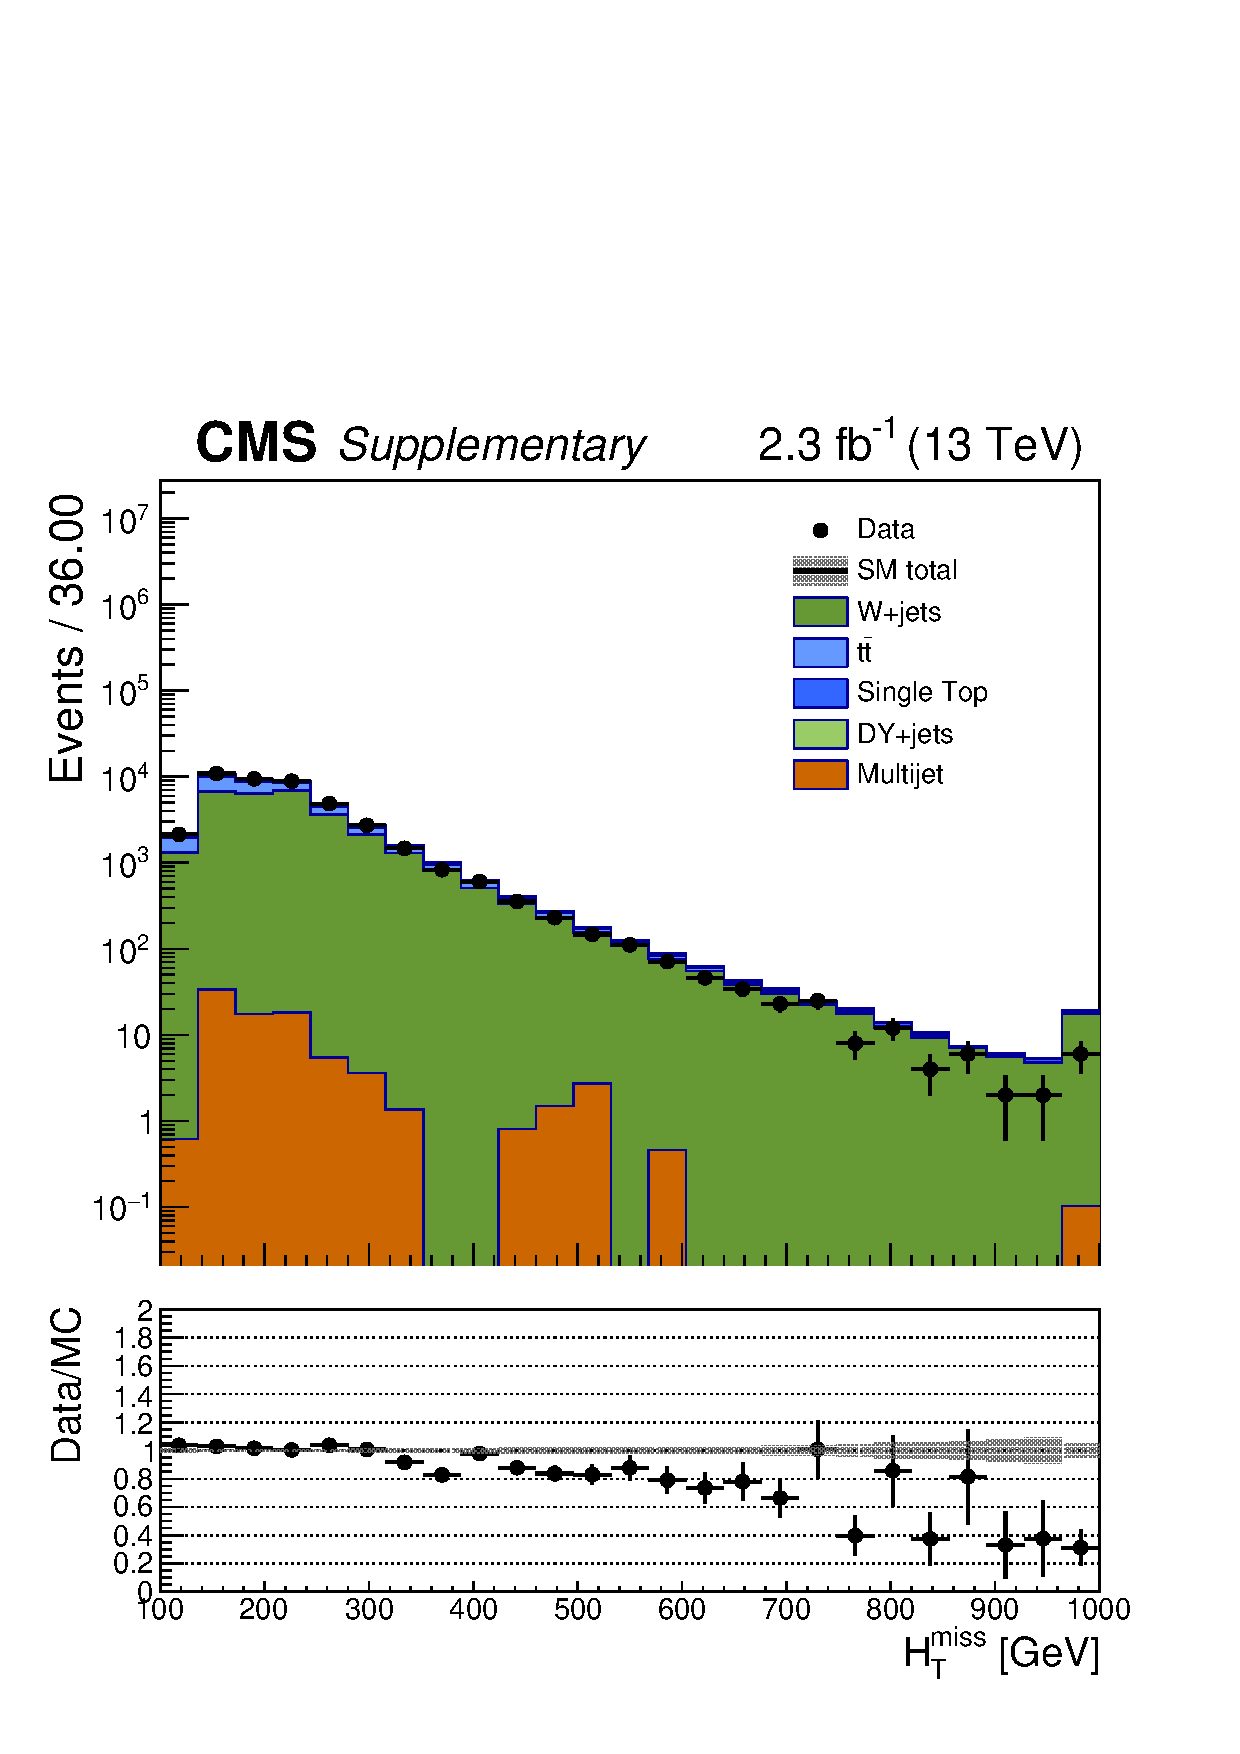
\includegraphics[width=0.45\textwidth]{figures/SingleMu_mht40_pt_all_all} \\
     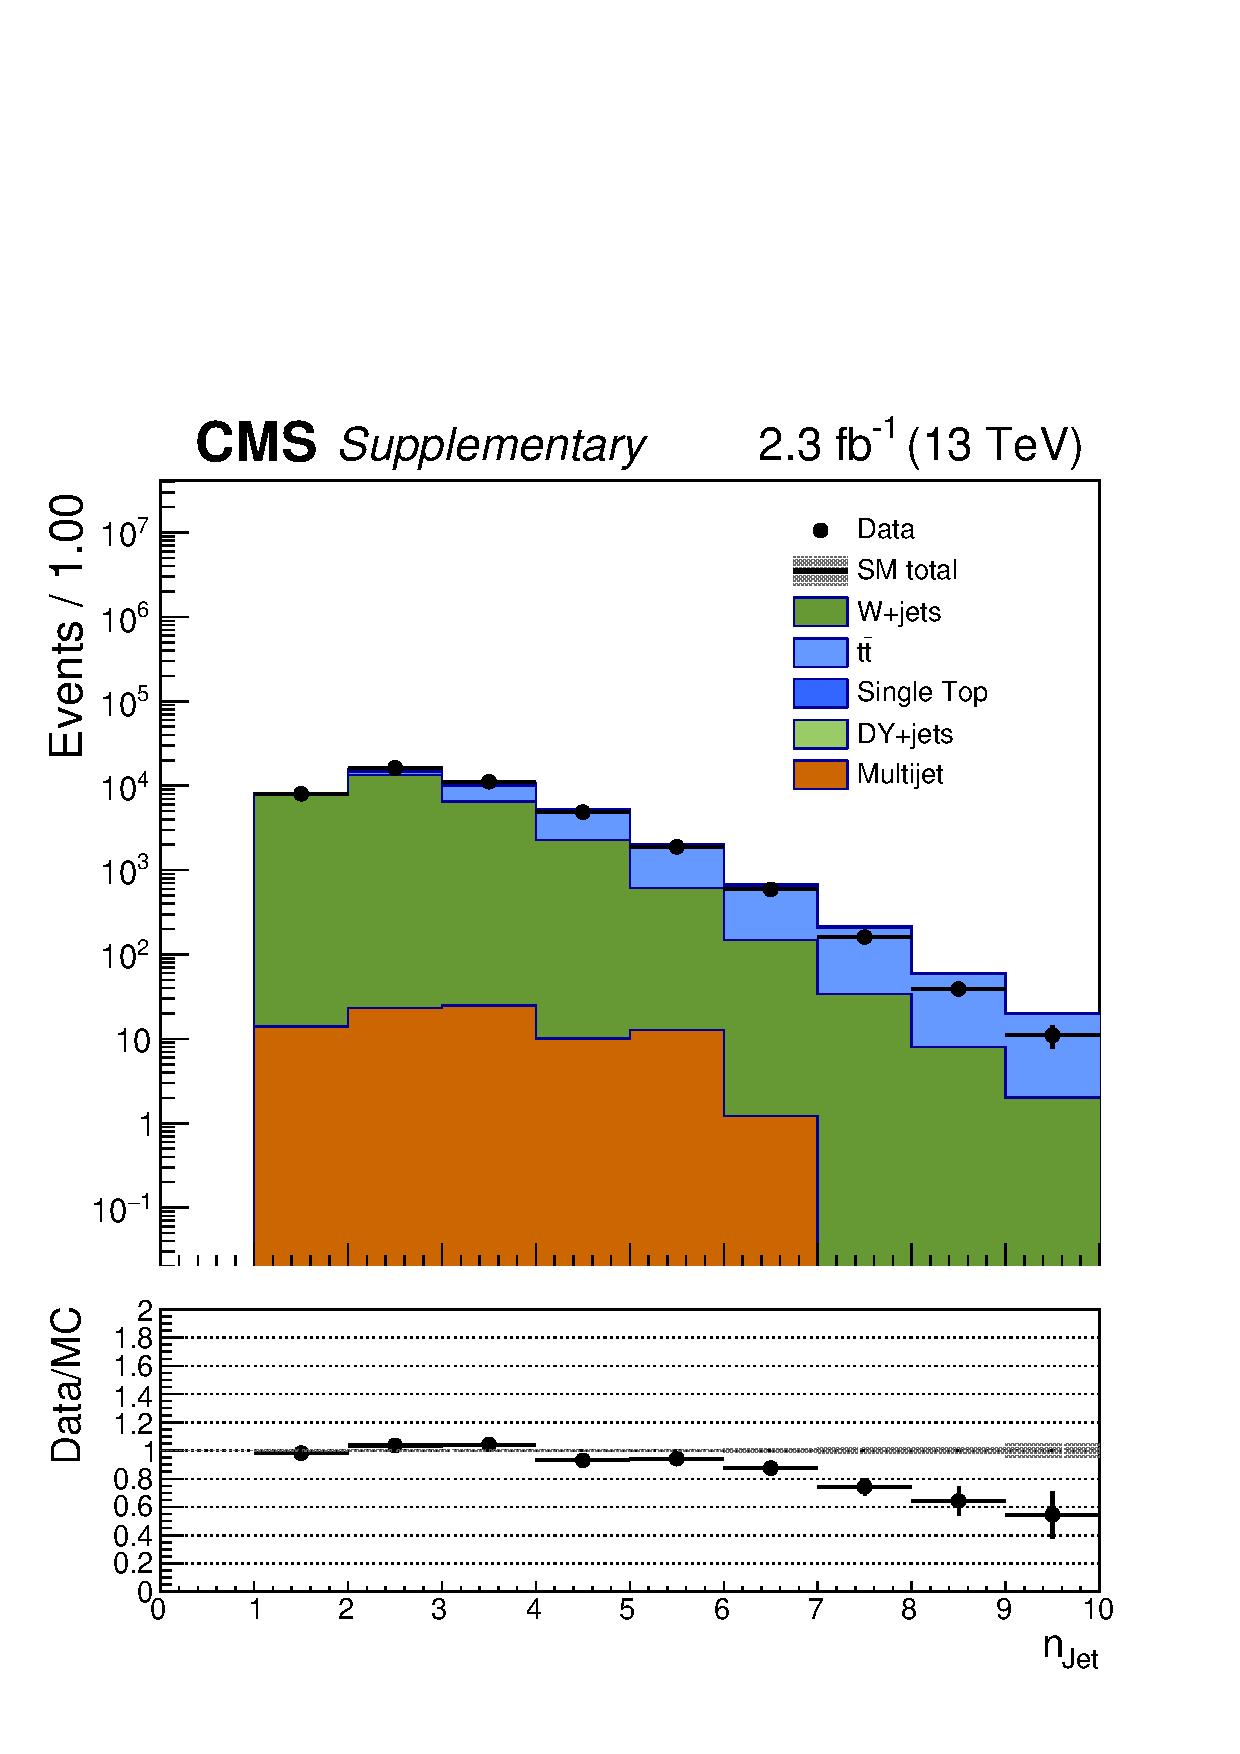
\includegraphics[width=0.45\textwidth]{figures/SingleMu_nJet40_all_all} ~~
     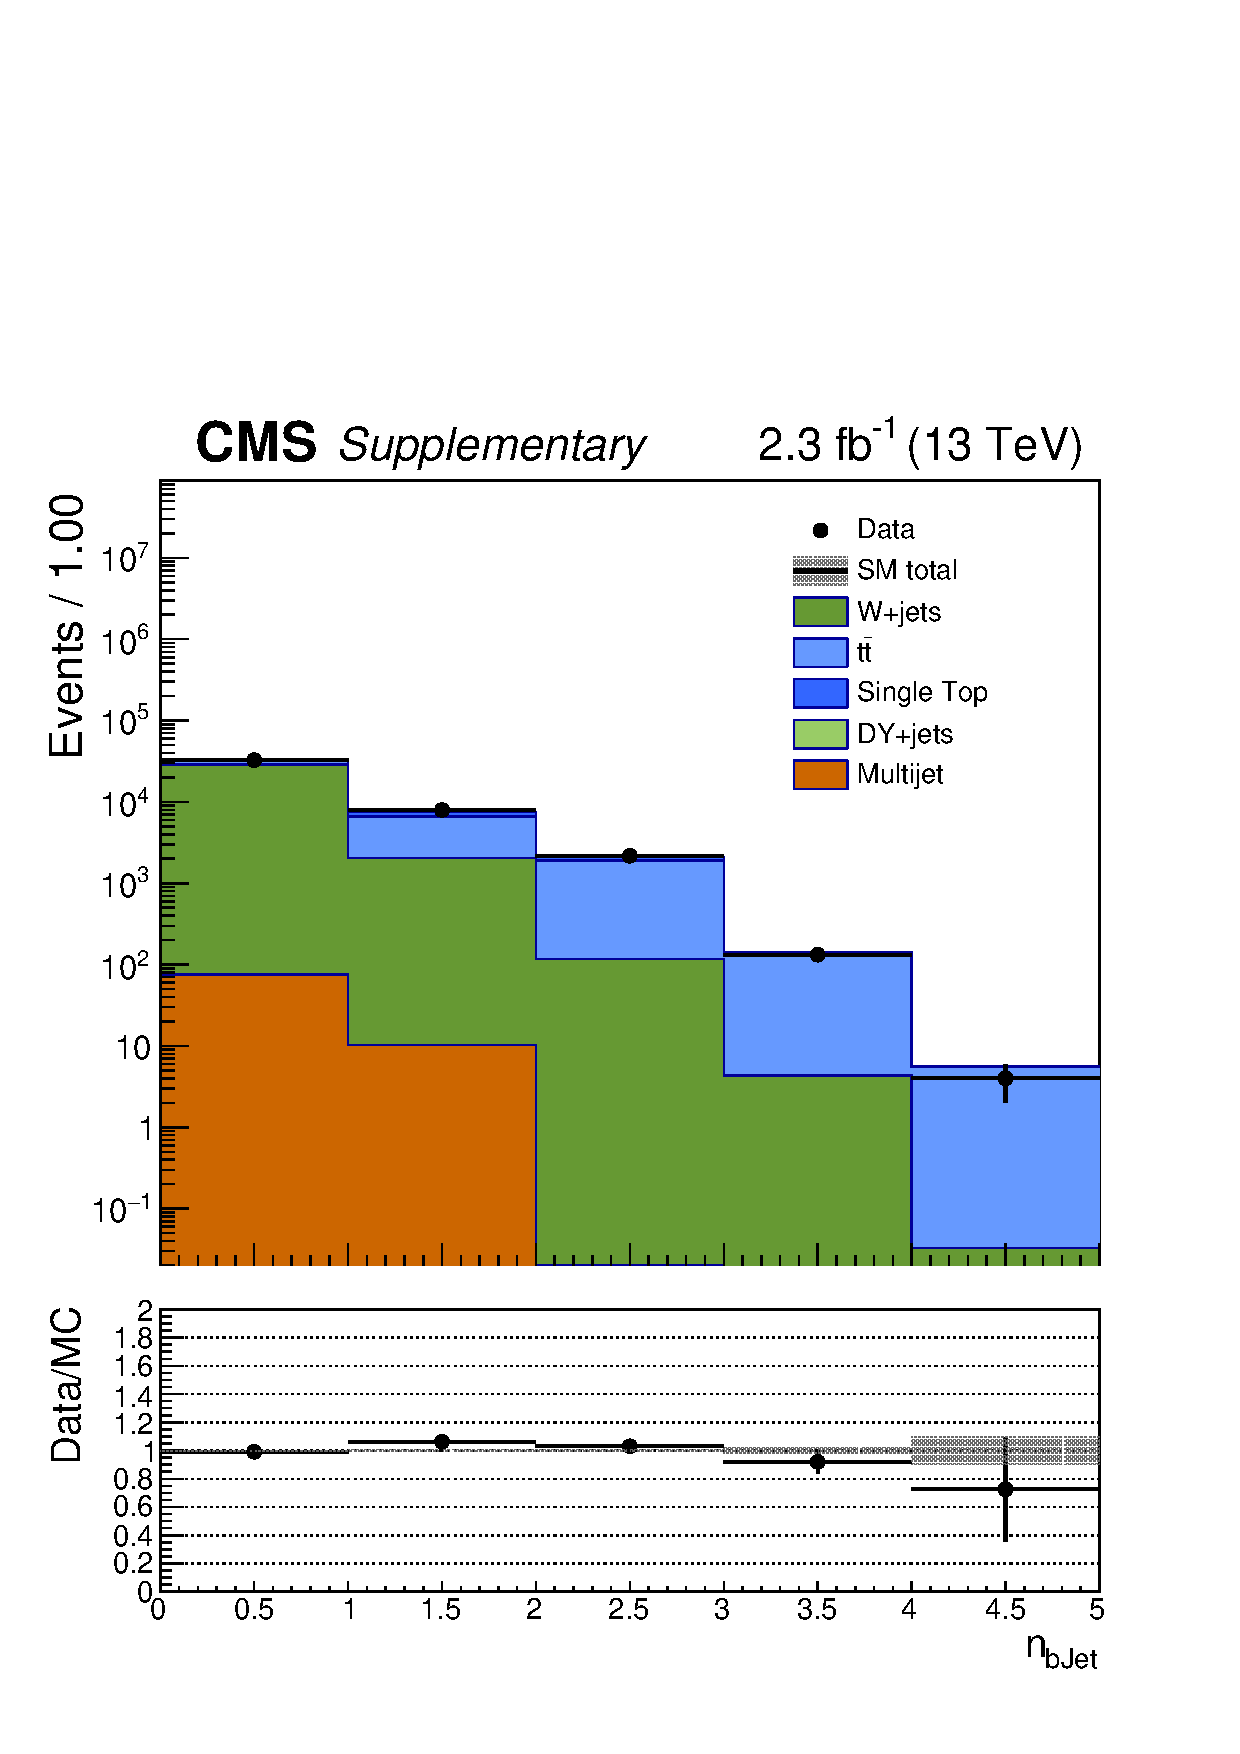
\includegraphics[width=0.45\textwidth]{figures/SingleMu_nBJet40_all_all} \\
  \end{center}
\end{figure}



\clearpage
\begin{figure}[tbhp]
    \caption{ 
    Distributions of data and MC predictions for \scalht (top left), \mht (top right), \nj (bottom left) and \nb (bottom right) 
    for the $\gamma+\mathrm{jets}$ control region. 
    It should be kept in mind that the analysis doesn't rely directly on simulation to derive the backgrounds, 
    so these plots are meant to show the shape of some of the variables used in the analysis despite the limitations 
    of the MC modelling. 
    \label{fig:data-MC_plots_SinglePhoton} }
  \begin{center}
     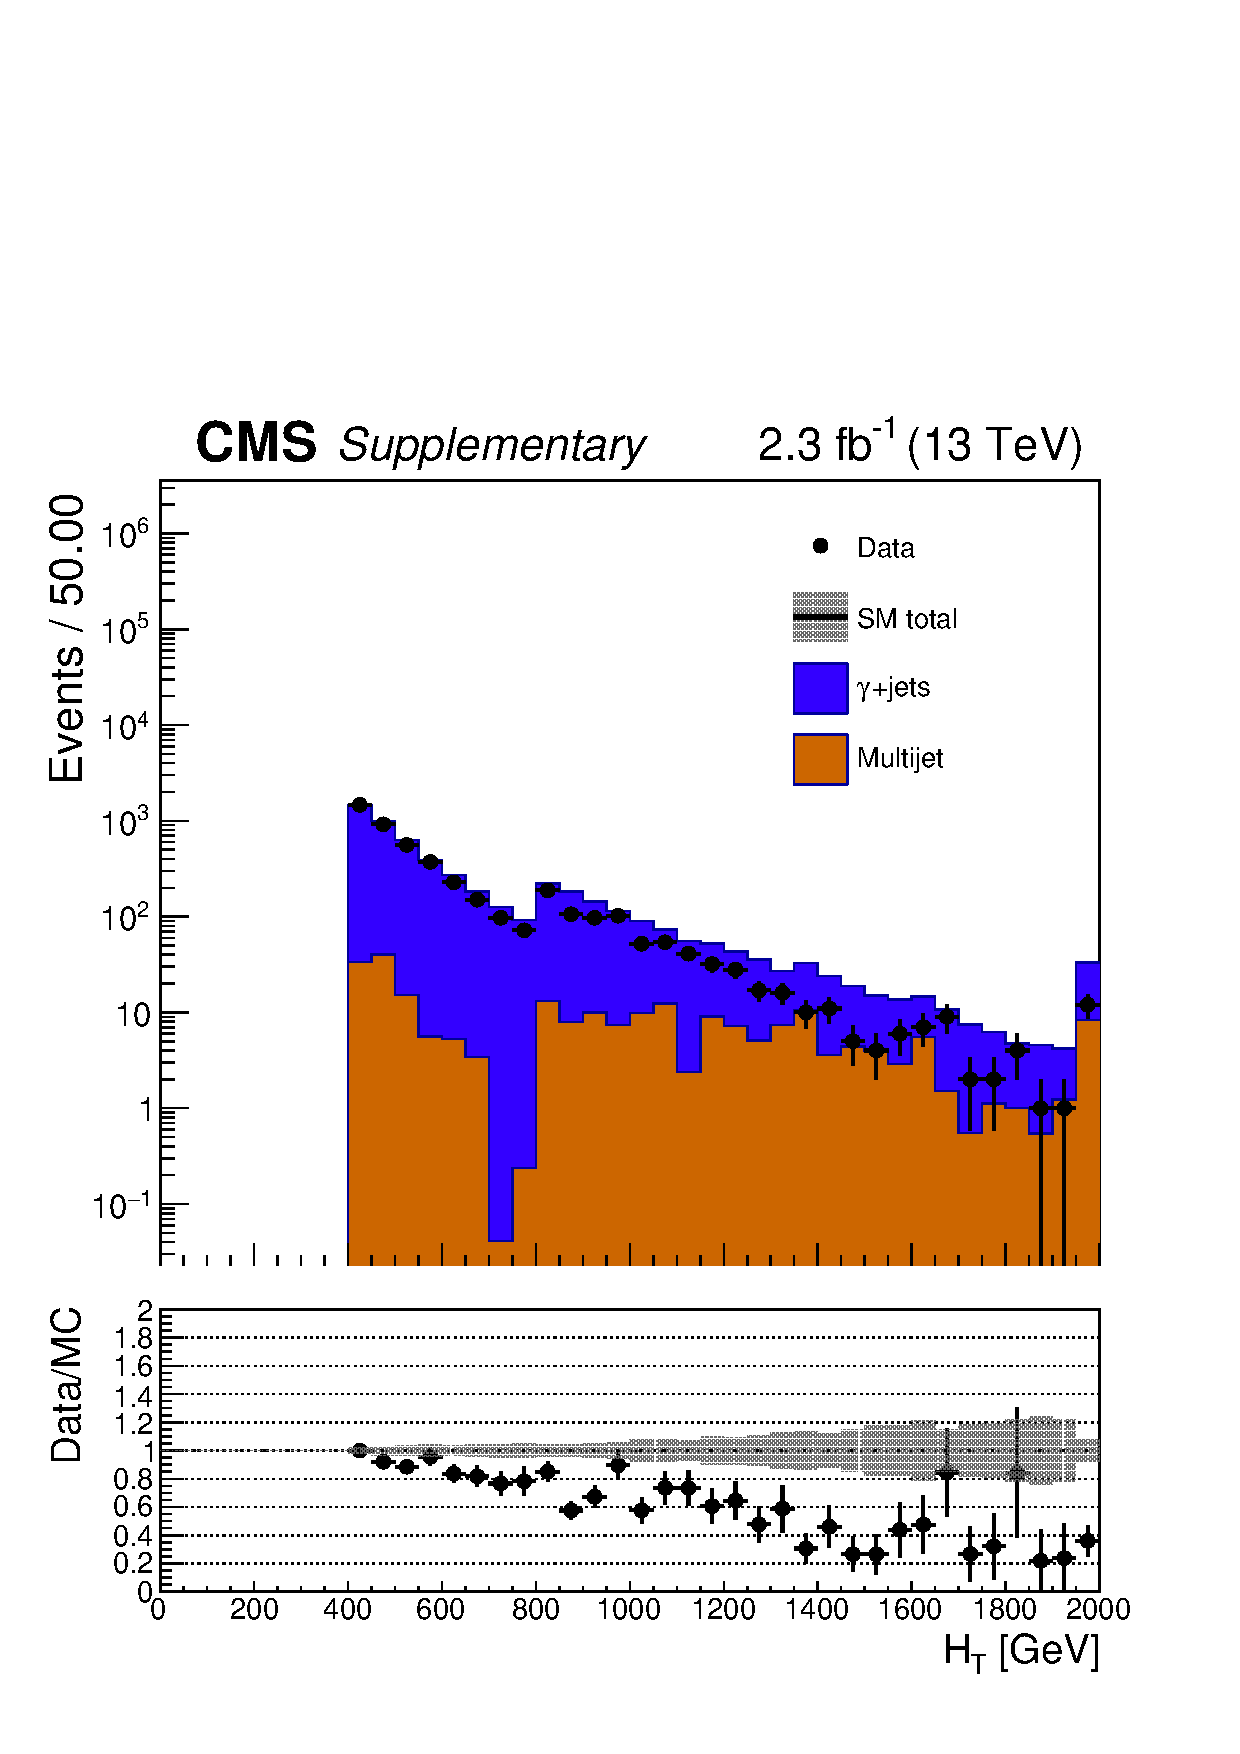
\includegraphics[width=0.45\textwidth]{figures/SinglePhoton_ht40_all_all} ~~
     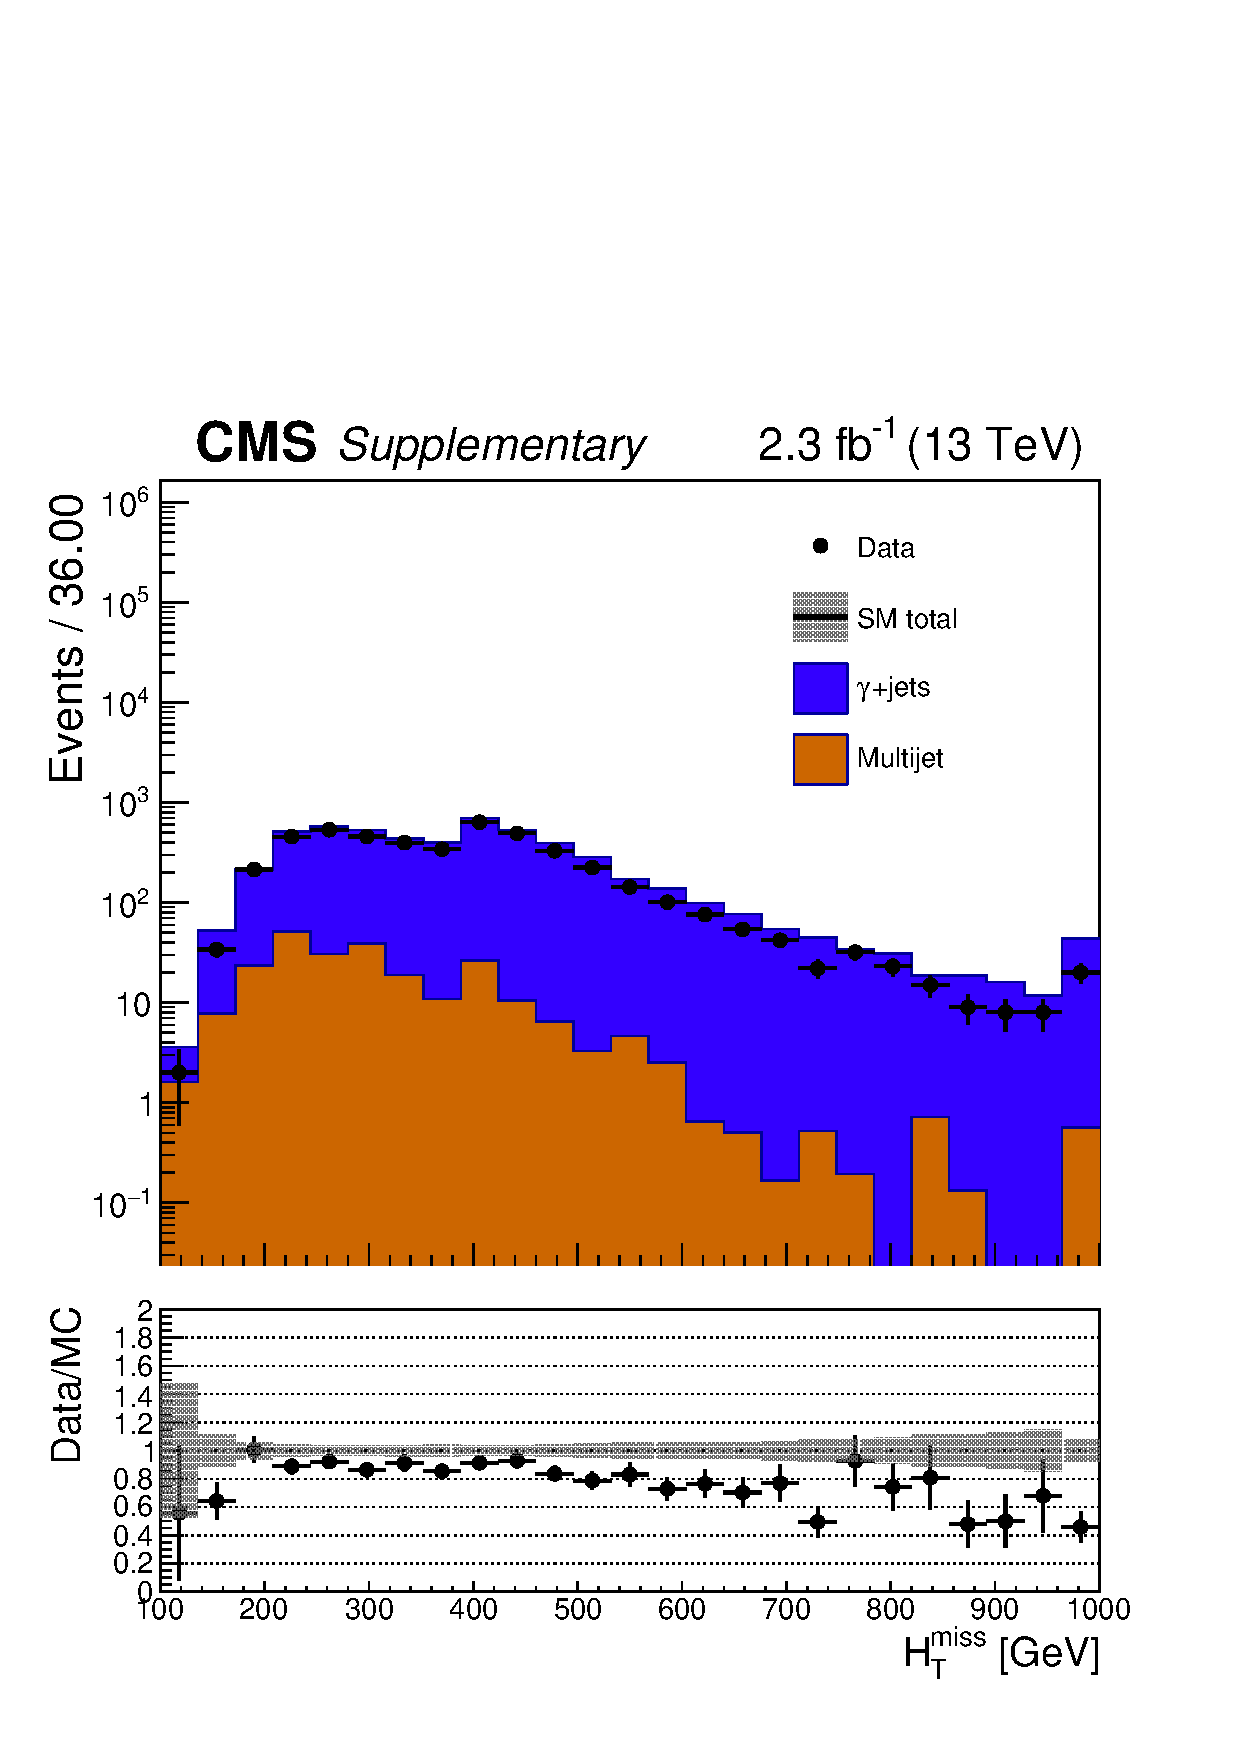
\includegraphics[width=0.45\textwidth]{figures/SinglePhoton_mht40_pt_all_all} \\
     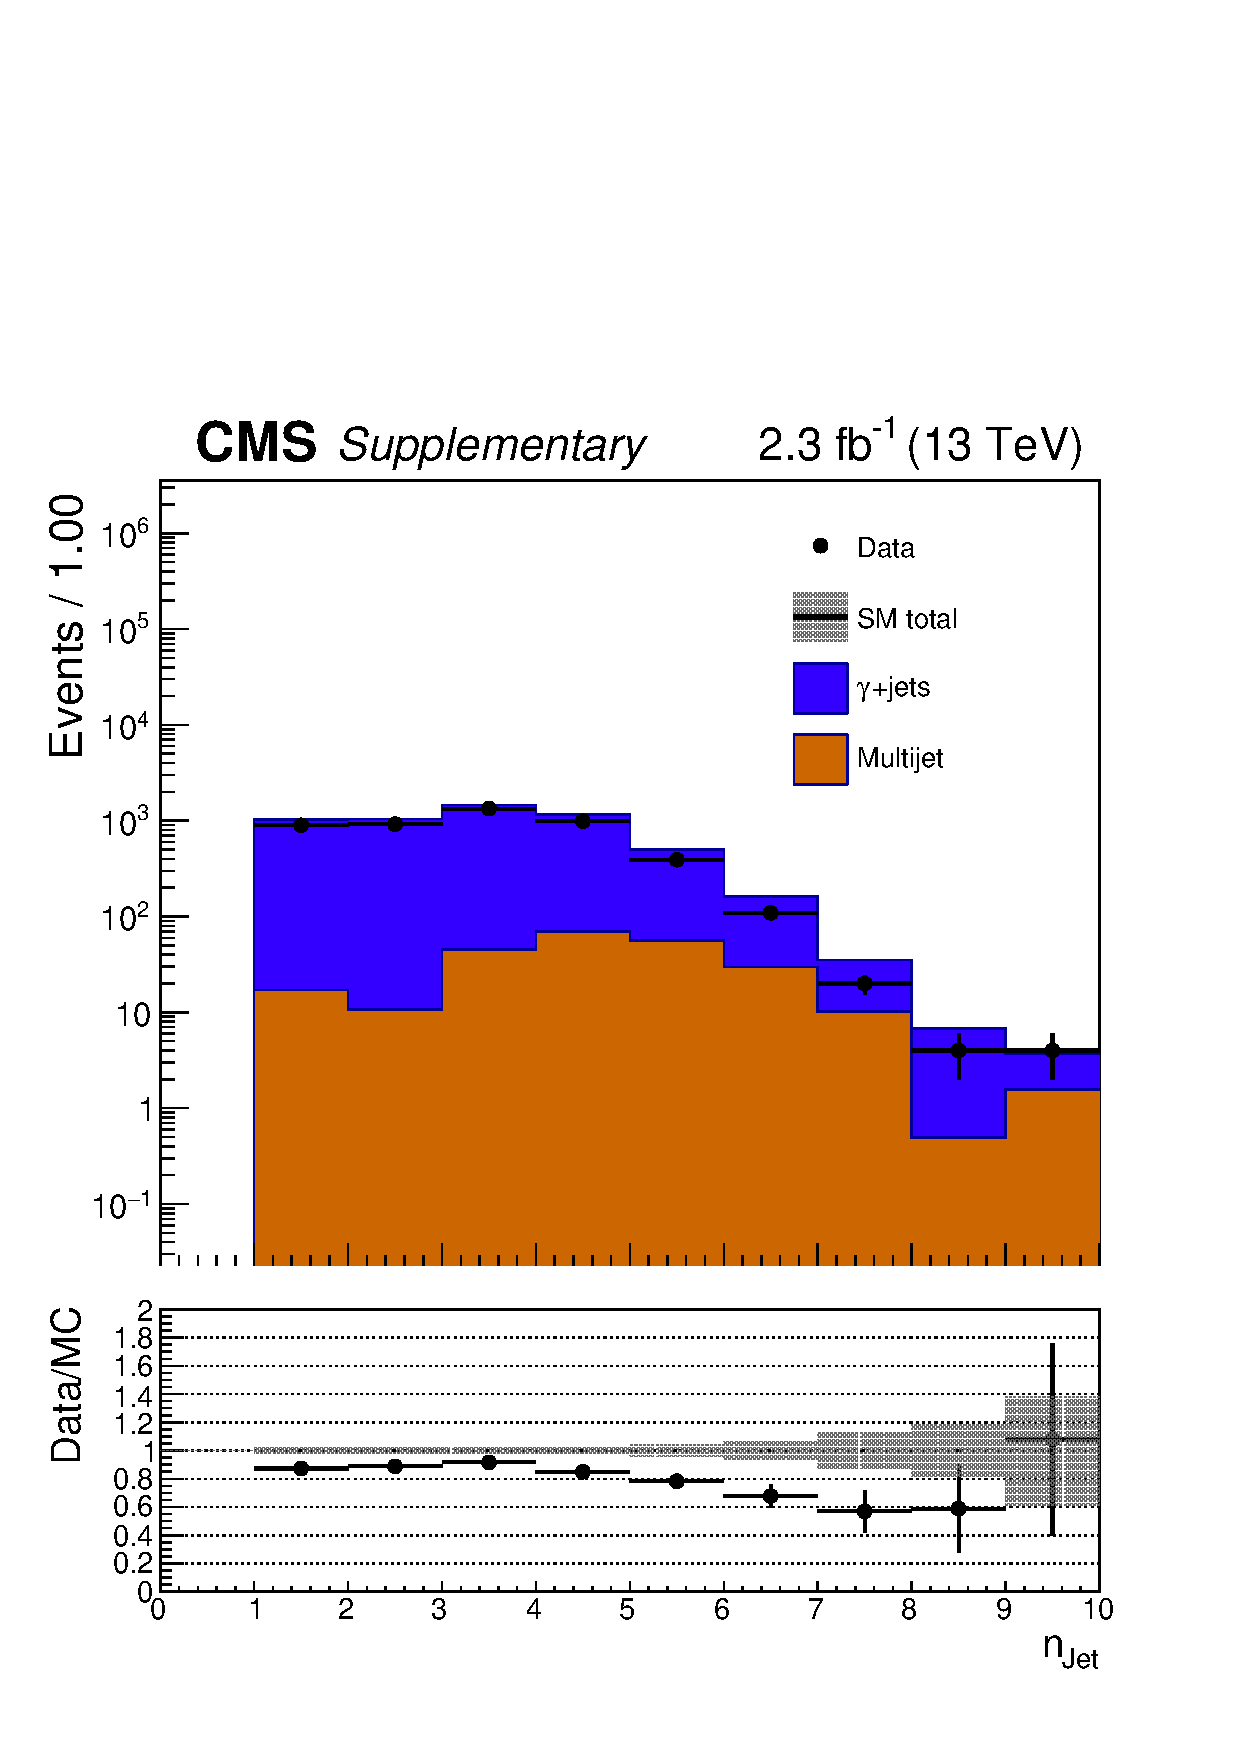
\includegraphics[width=0.45\textwidth]{figures/SinglePhoton_nJet40_all_all} ~~
     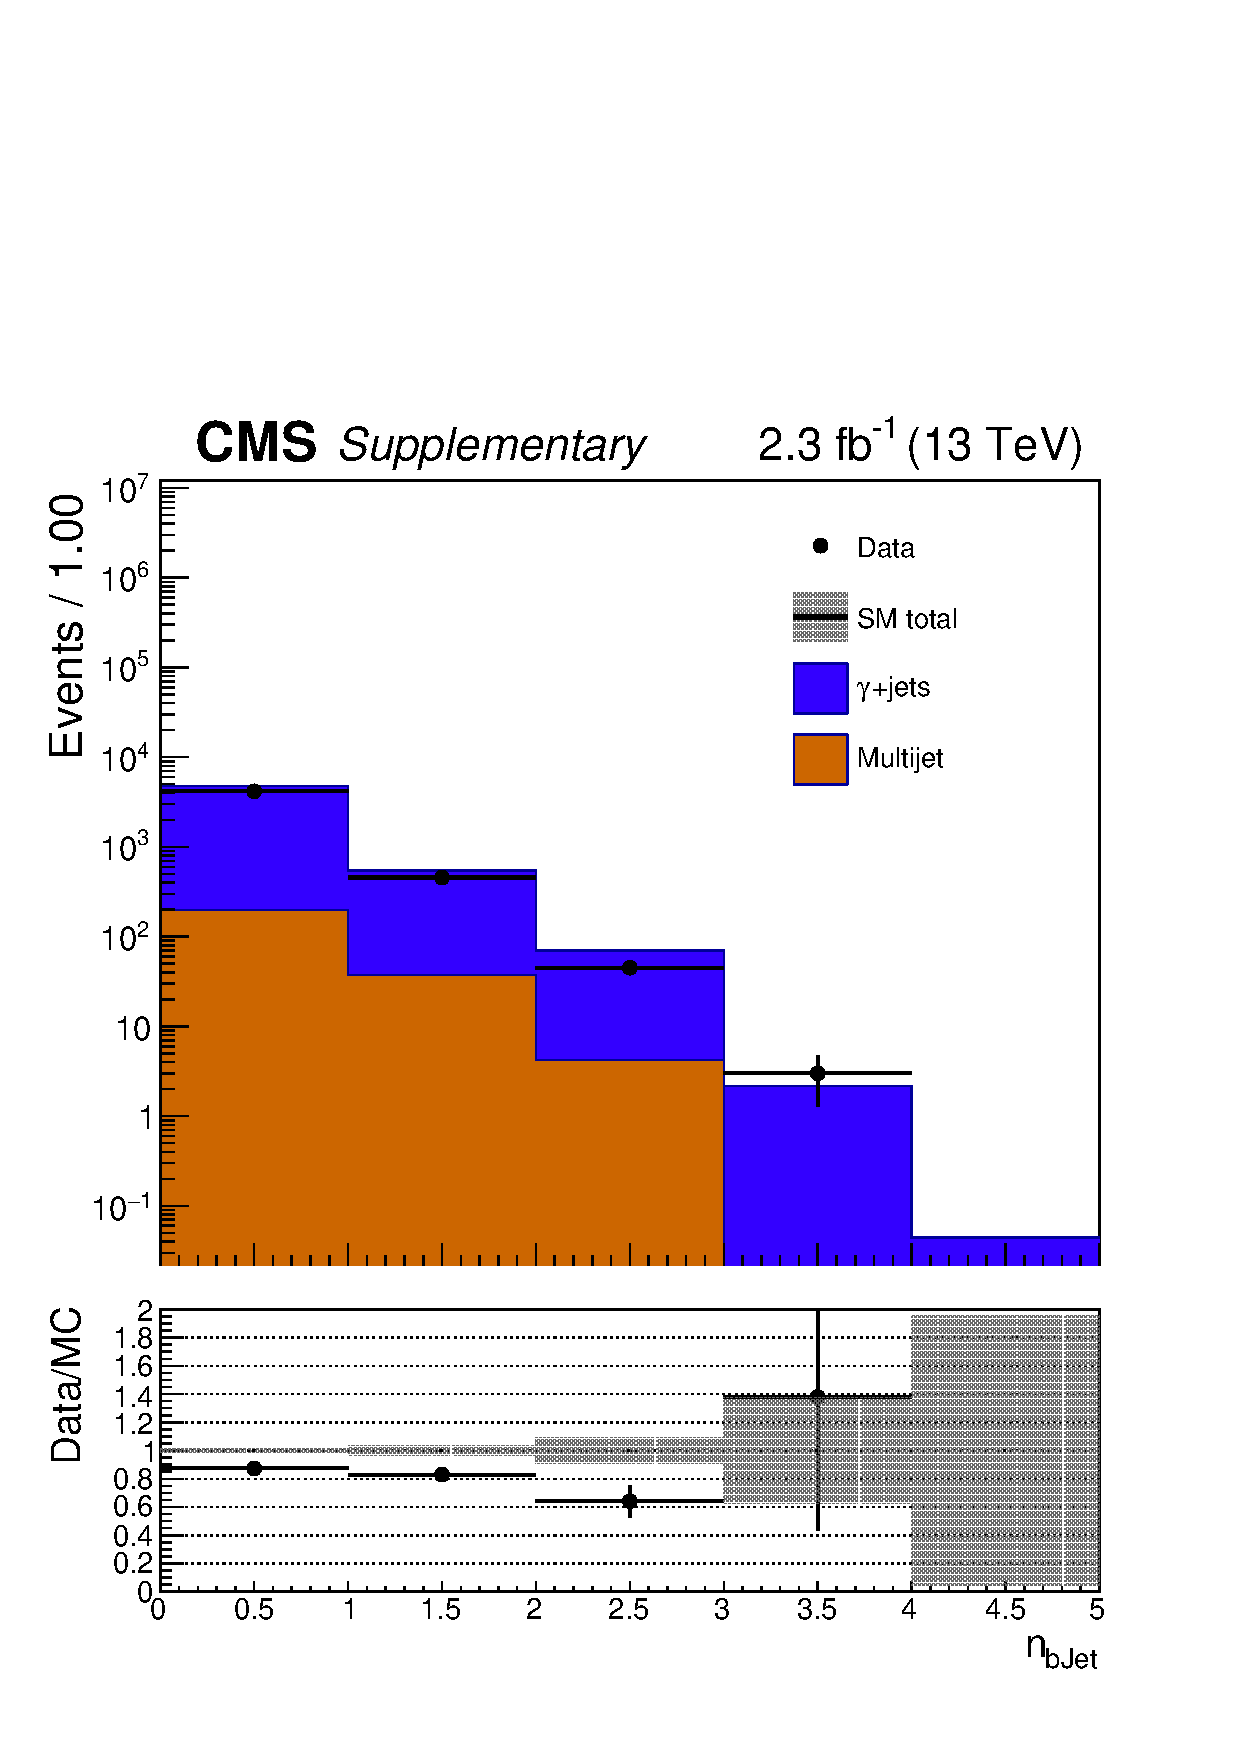
\includegraphics[width=0.45\textwidth]{figures/SinglePhoton_nBJet40_all_all} \\
  \end{center}
\end{figure}


\clearpage
\begin{figure}[tbhp]
    \caption{ 
    Distributions of data and MC predictions for \scalht (top left), \mht (top right), \nj (bottom left) and \nb (bottom right) 
    for the $\mu\mu+\mathrm{jets}$ control region. 
    It should be kept in mind that the analysis doesn't rely directly on simulation to derive the backgrounds, 
    so these plots are meant to show the shape of some of the variables used in the analysis despite the limitations 
    of the MC modelling. 
    \label{fig:data-MC_plots_DoubleMu} }
  \begin{center}
     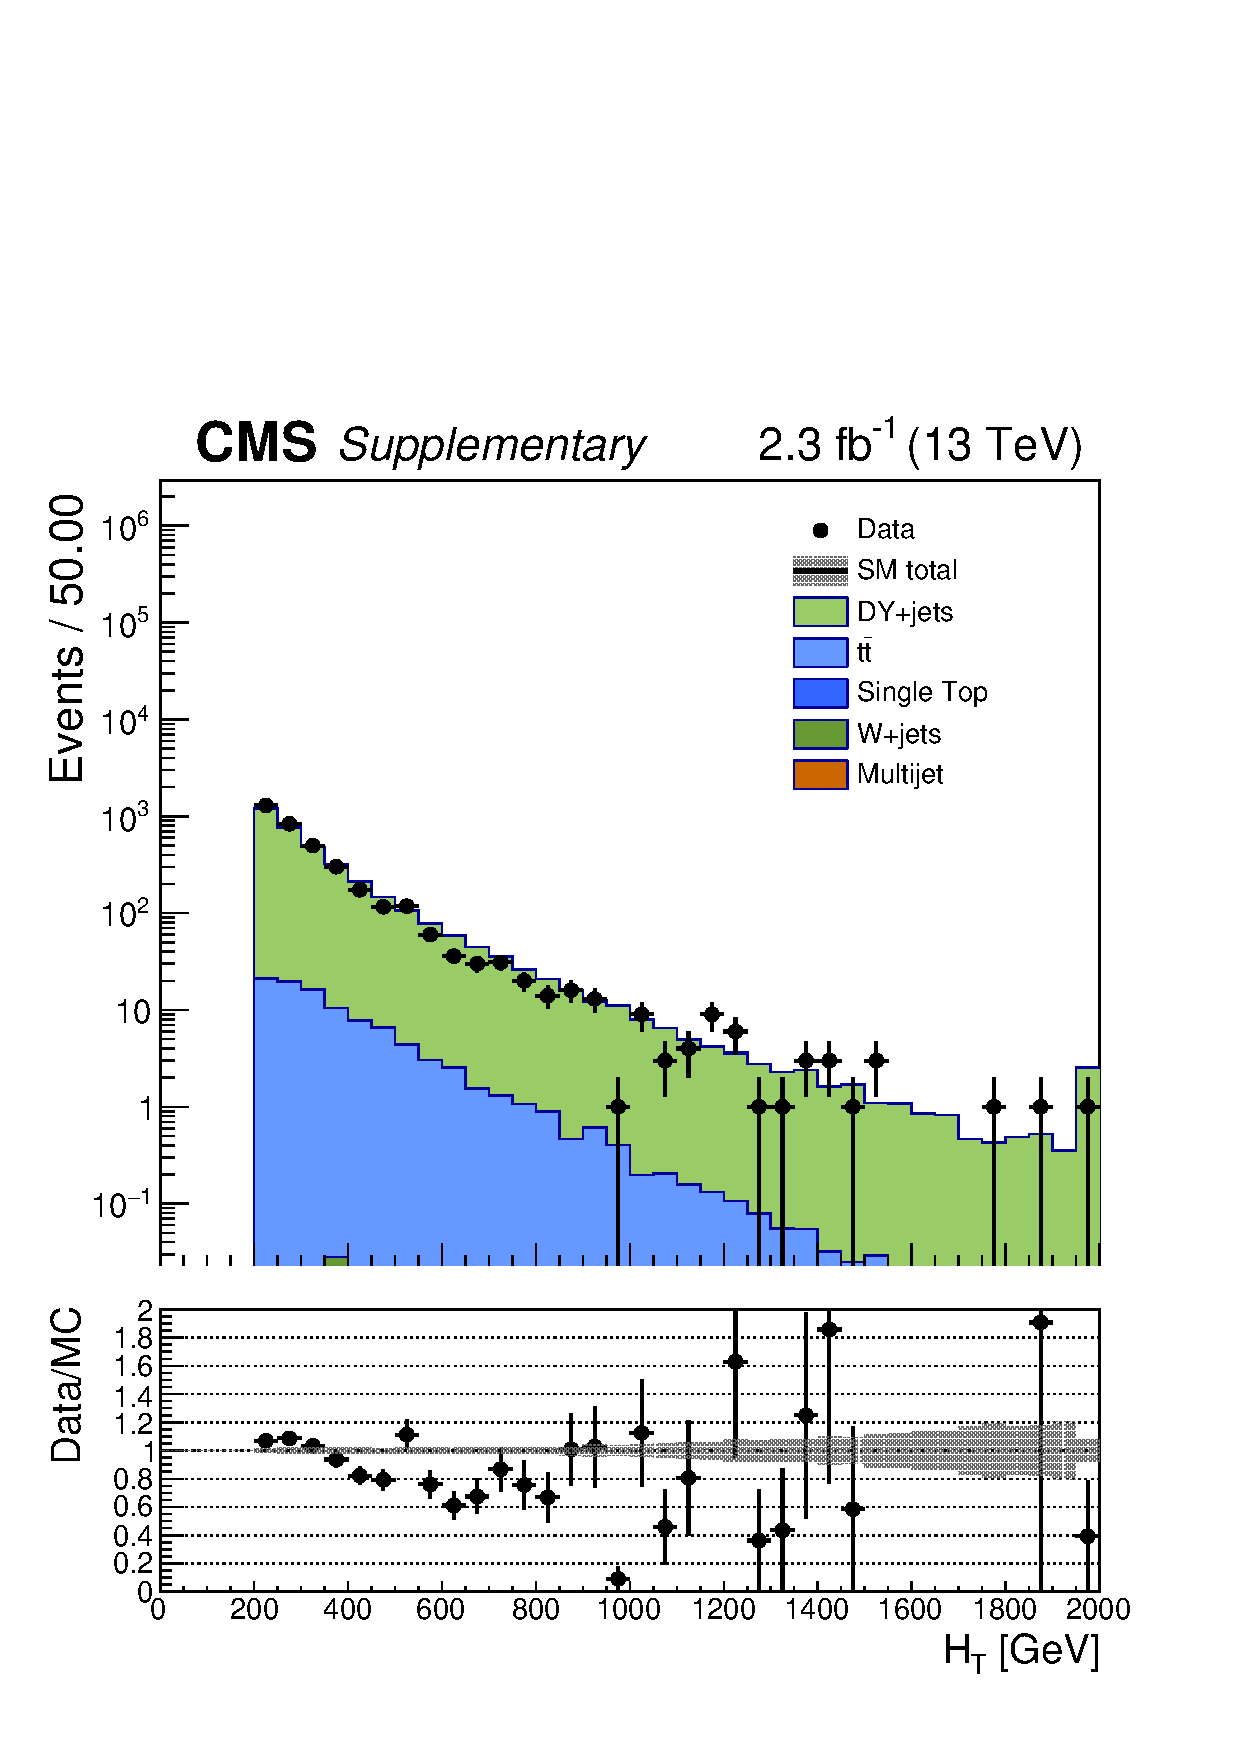
\includegraphics[width=0.45\textwidth]{figures/DoubleMu_ht40_all_all} ~~
     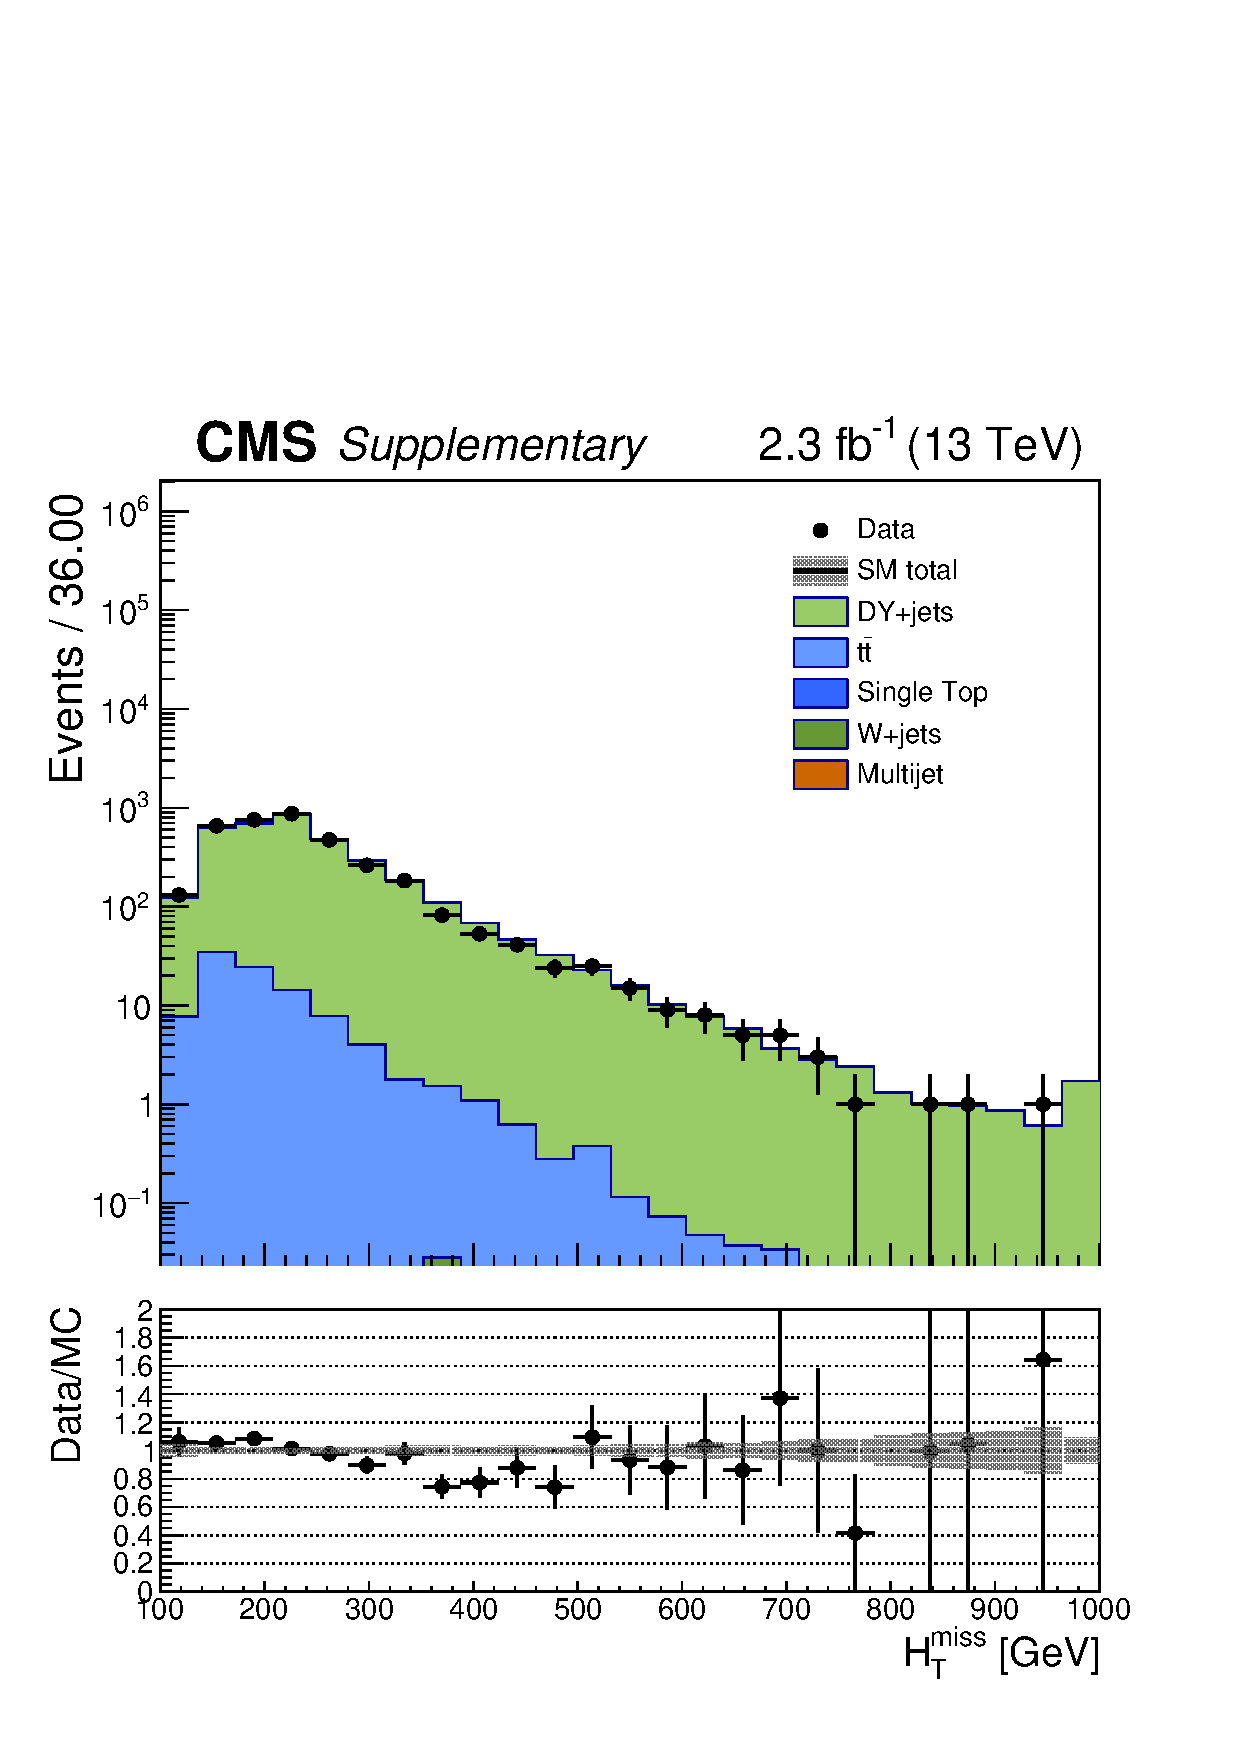
\includegraphics[width=0.45\textwidth]{figures/DoubleMu_mht40_pt_all_all} \\
     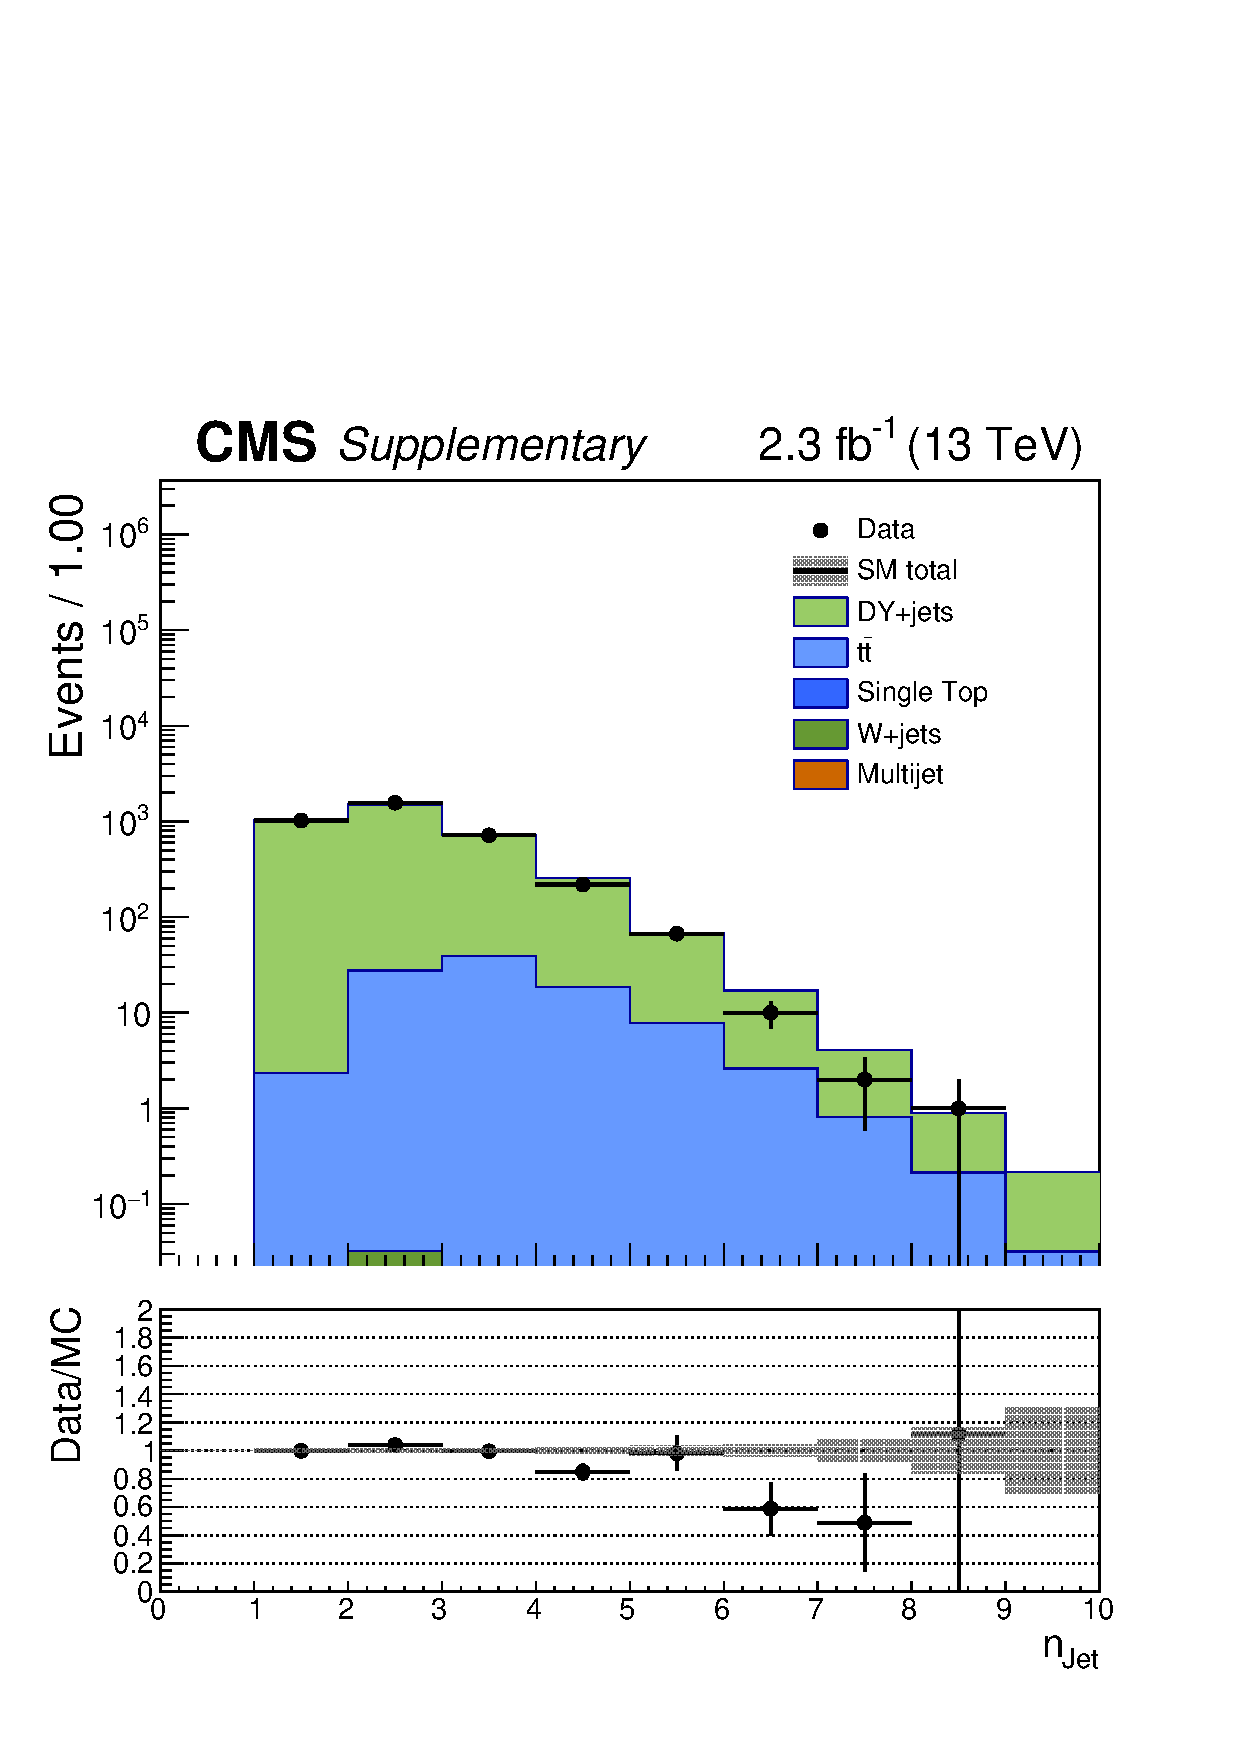
\includegraphics[width=0.45\textwidth]{figures/DoubleMu_nJet40_all_all} ~~
     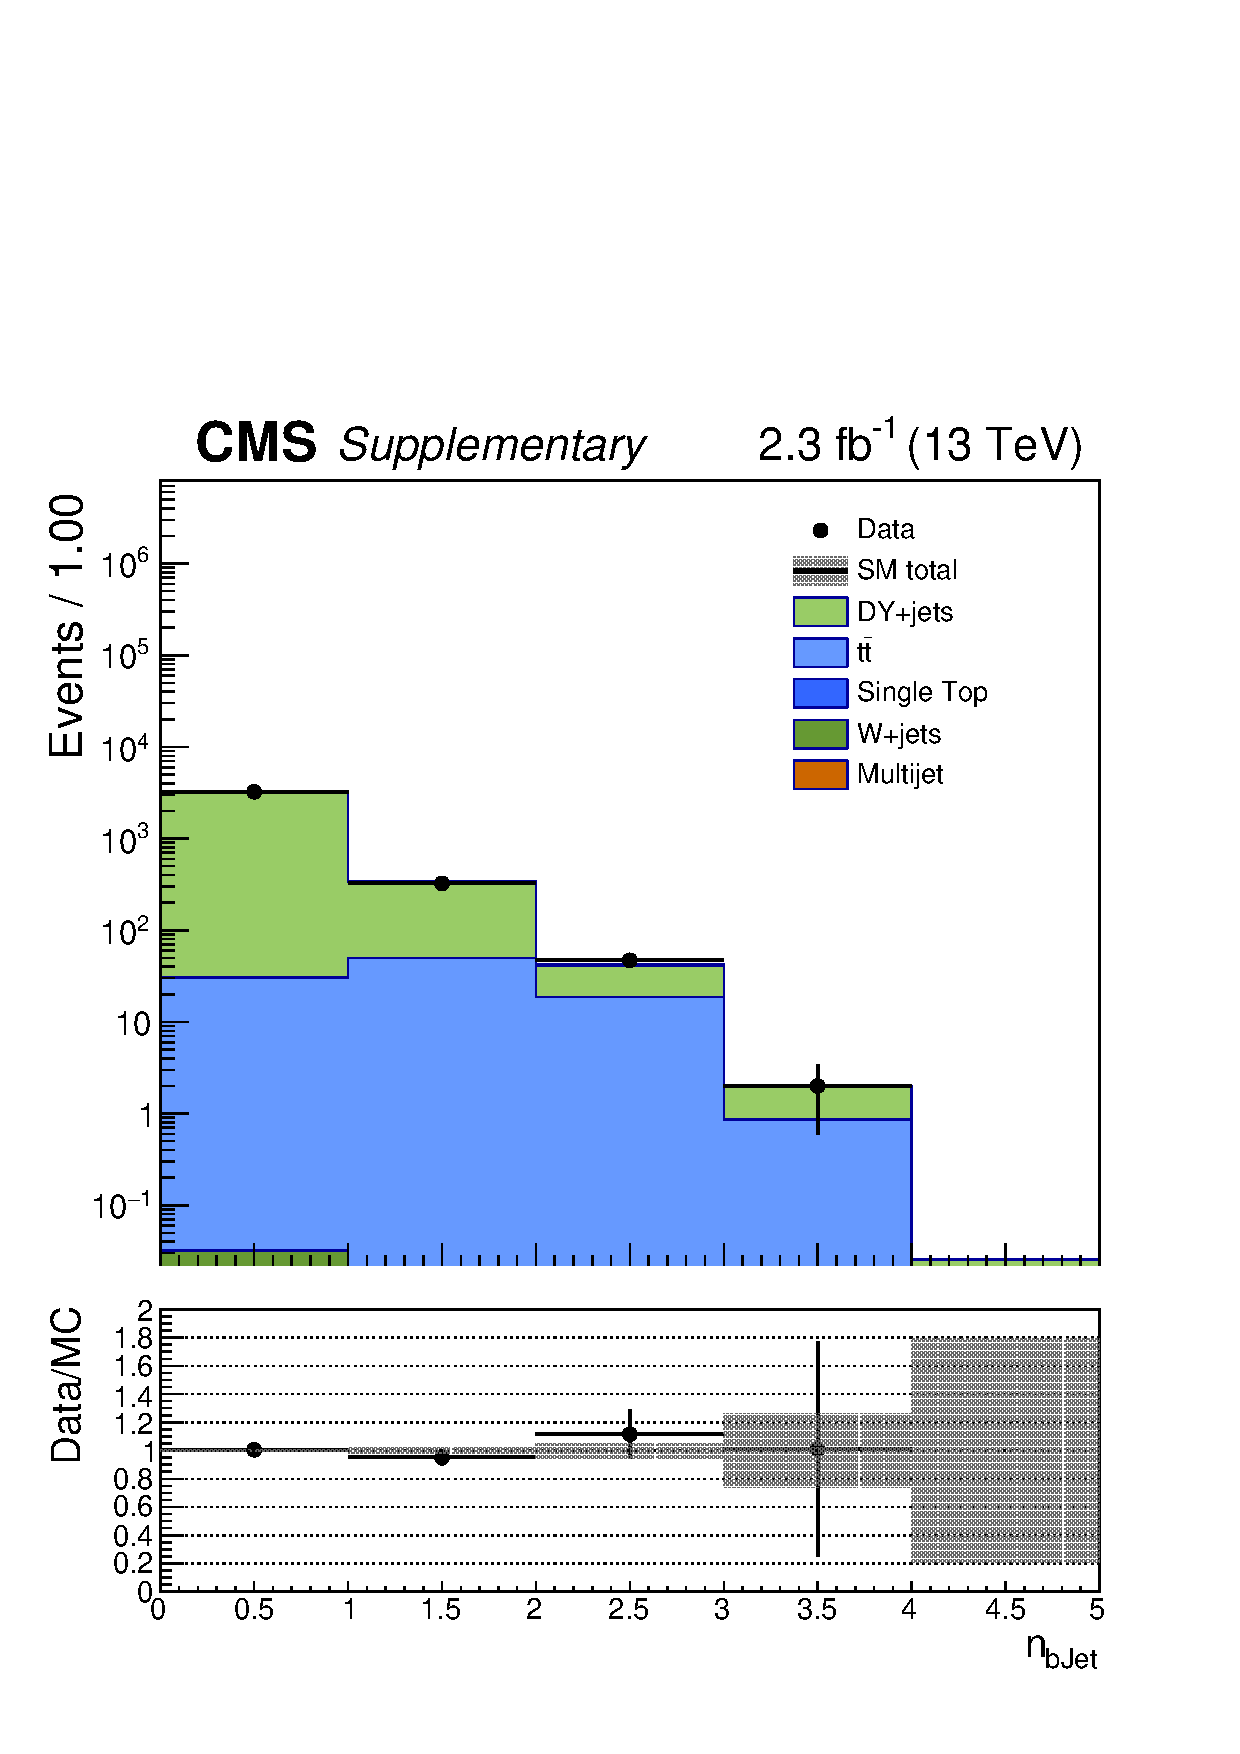
\includegraphics[width=0.45\textwidth]{figures/DoubleMu_nBJet40_all_all} \\
  \end{center}
\end{figure}


\clearpage
\begin{figure}[tbhp]
    \caption{ 
  Data-driven test of the \alt extrapolation for the symmetric (left) and asymmetric (right) jet categories. 
  In this test, the data yield in the \mj sample with $\alt>0.5$ ($N_{\mathrm{obs}}$) 
  is compared with the prediction obtained from the \mj sample with $\alt<0.5$ multiplied by the corresponding 
  transfer factor computed in simulation ($N_{\mathrm{pred}}$). 
  A systematic uncertainty (grey band) is derived, as a function of \scalht and separately for symmetric and asymmetric categories, 
  to cover the non-closure. 
    \label{fig:CT-alphaT} }
  \begin{center}
     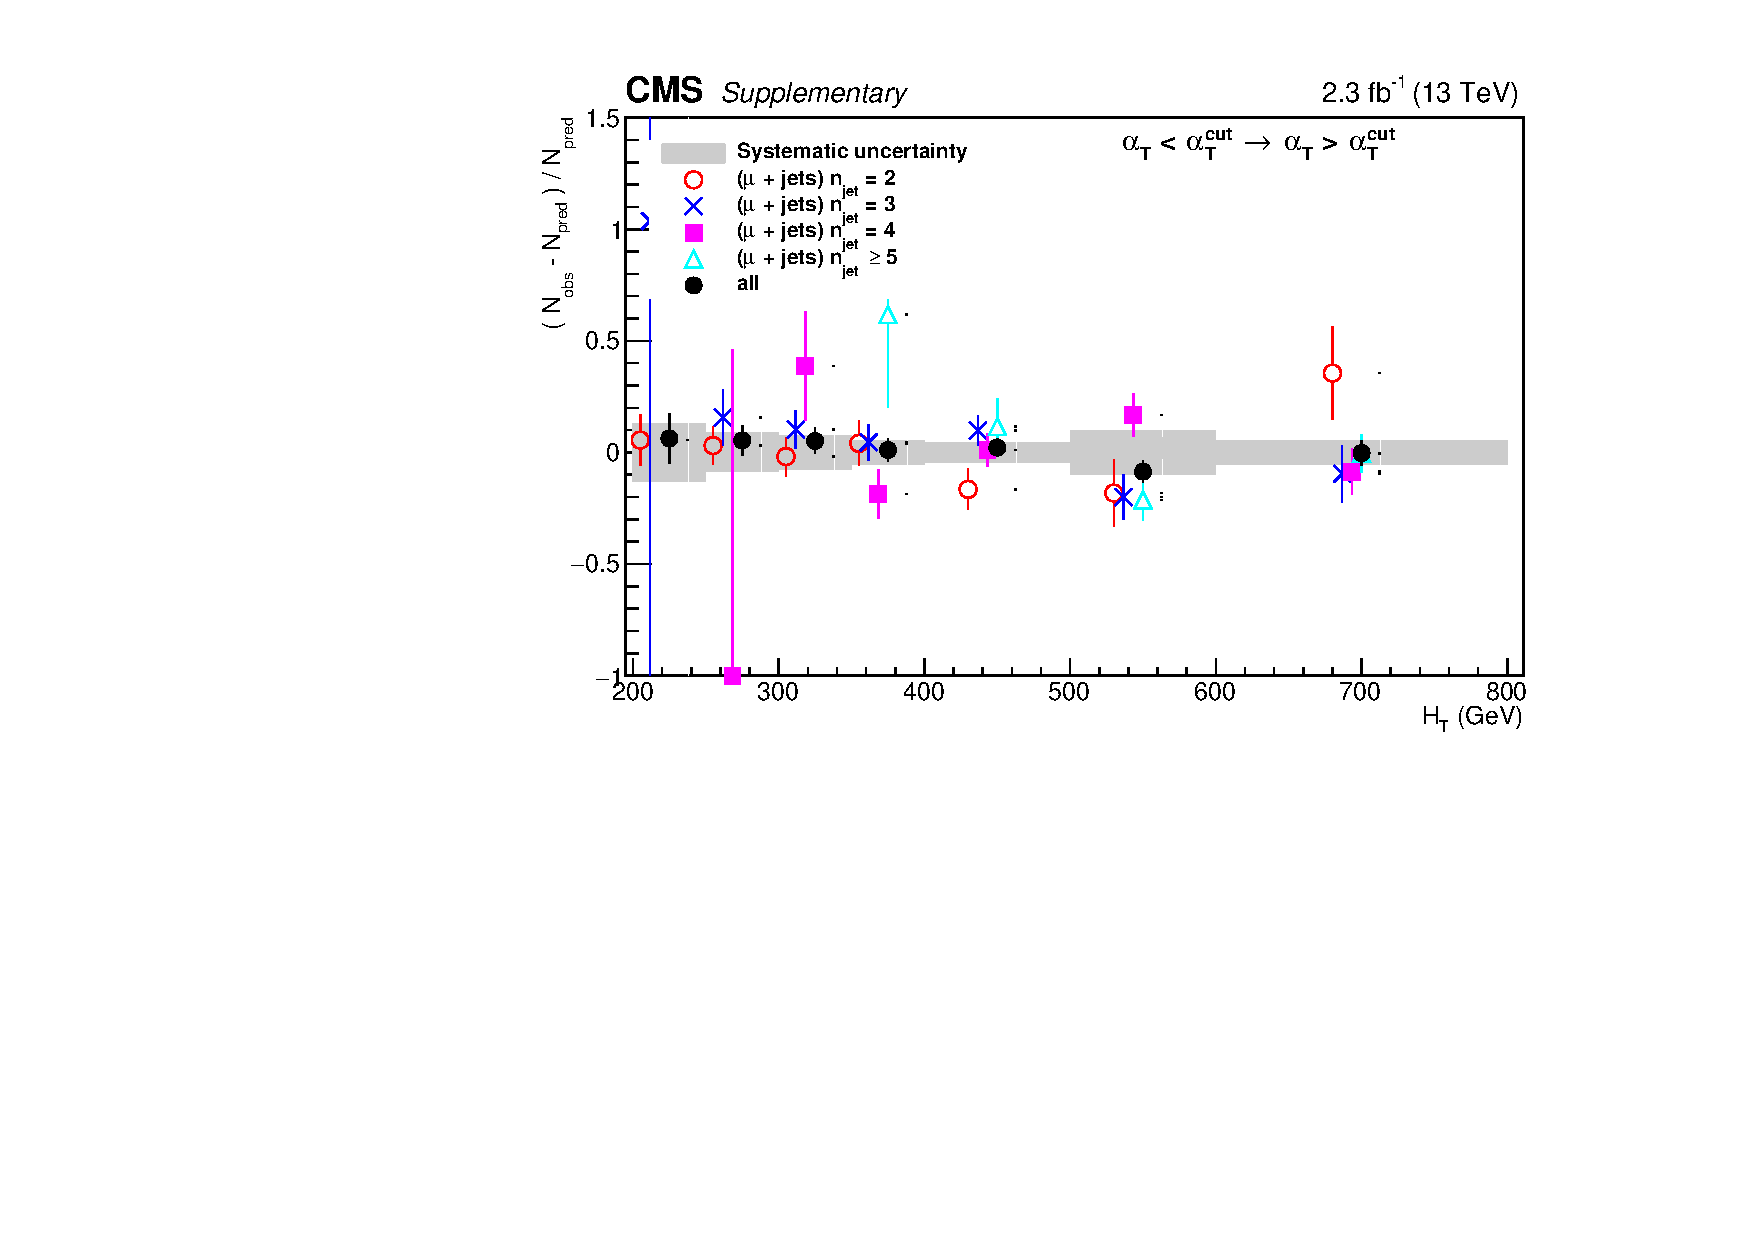
\includegraphics[width=0.48\textwidth]{figures/alphaTsym__noFit} ~~
     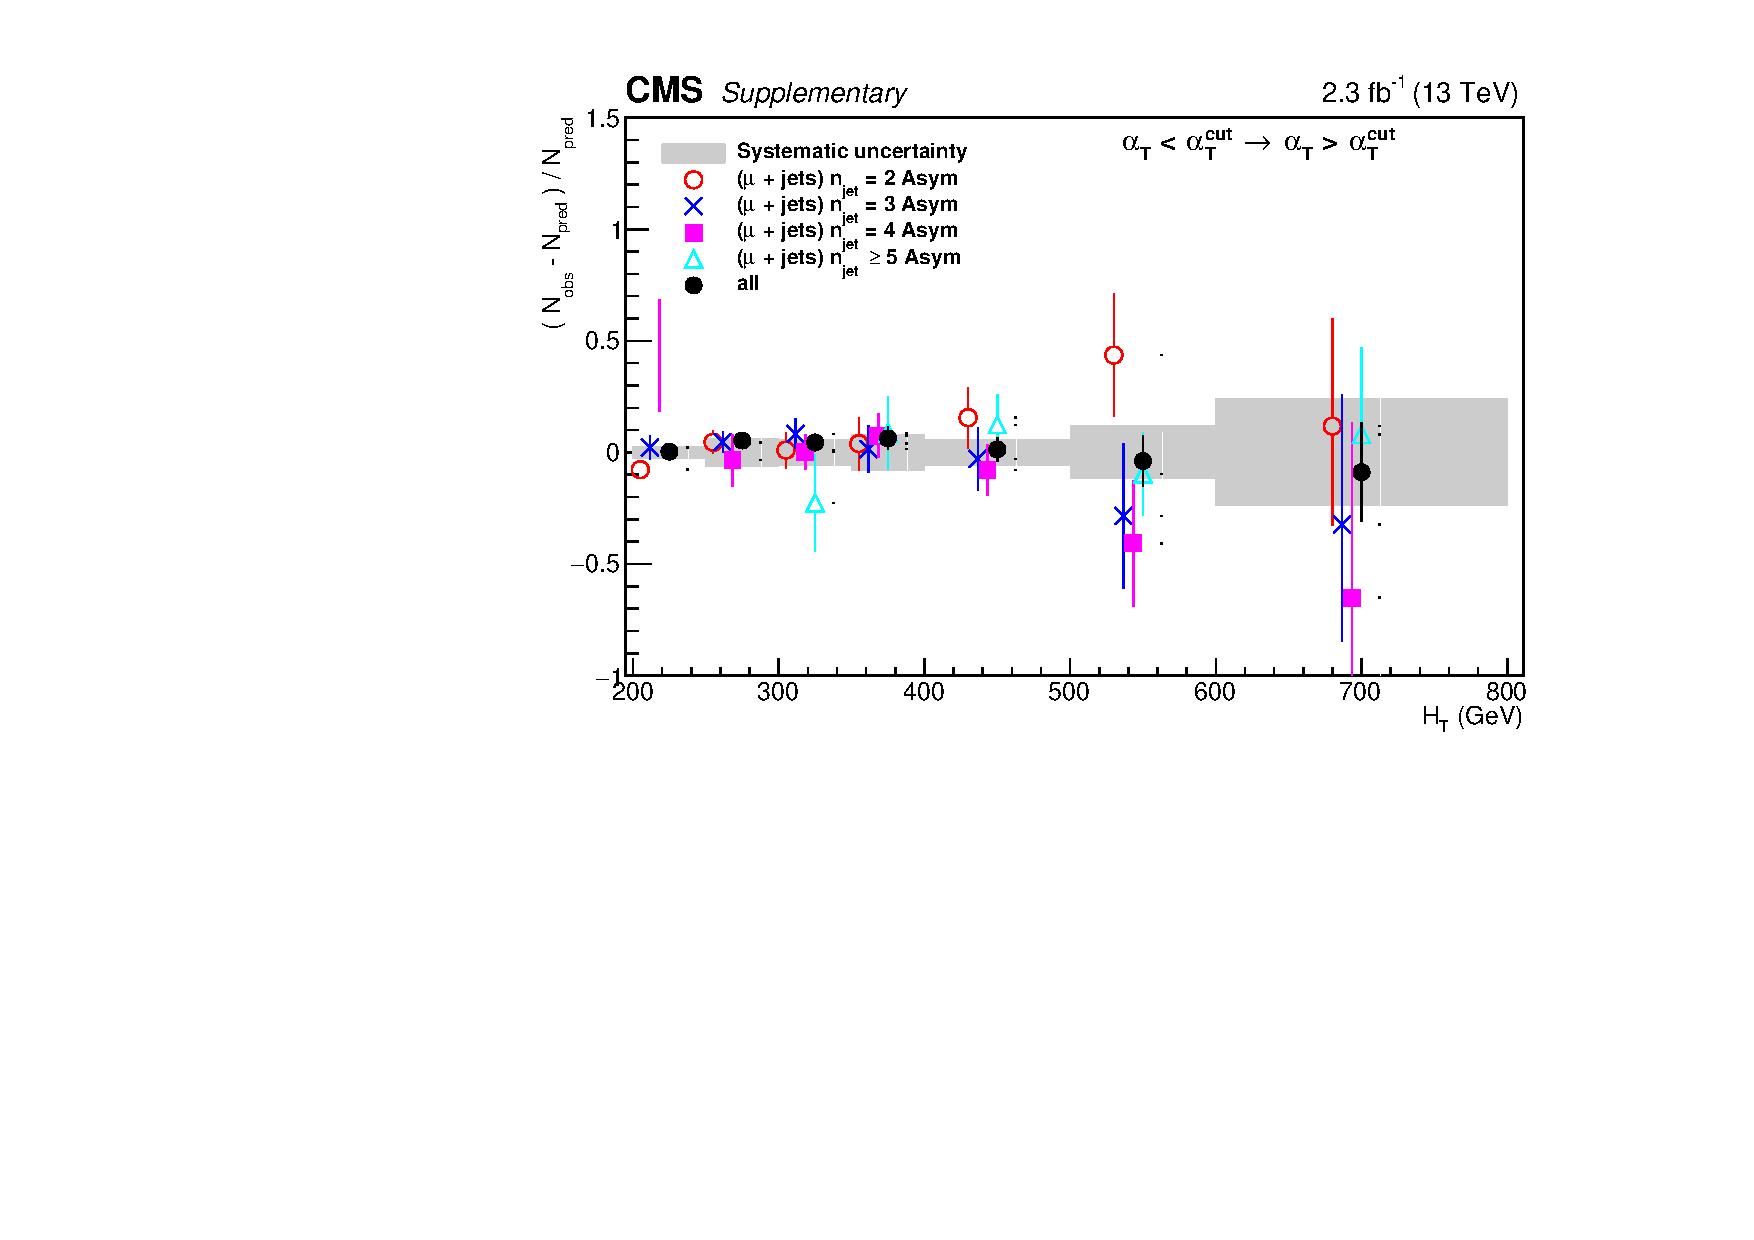
\includegraphics[width=0.48\textwidth]{figures/alphaTasym__noFit}
  \end{center}
\end{figure}

\begin{figure}[tbhp]
    \caption{ 
  Data-driven test of the modelling of the Z/W ratio for the symmetric (left) and asymmetric (right) jet categories. 
  In this test, the data yield in the \mmj sample ($N_{\mathrm{obs}}$) 
  is compared with the prediction obtained from the \mj sample multiplied by the corresponding 
  transfer factor computed in simulation ($N_{\mathrm{pred}}$). 
  A systematic uncertainty (grey band) is derived, as a function of \scalht and separately for symmetric and asymmetric categories, 
  to cover the non-closure. 
    \label{fig:CT-alphaT} }
  \begin{center}
     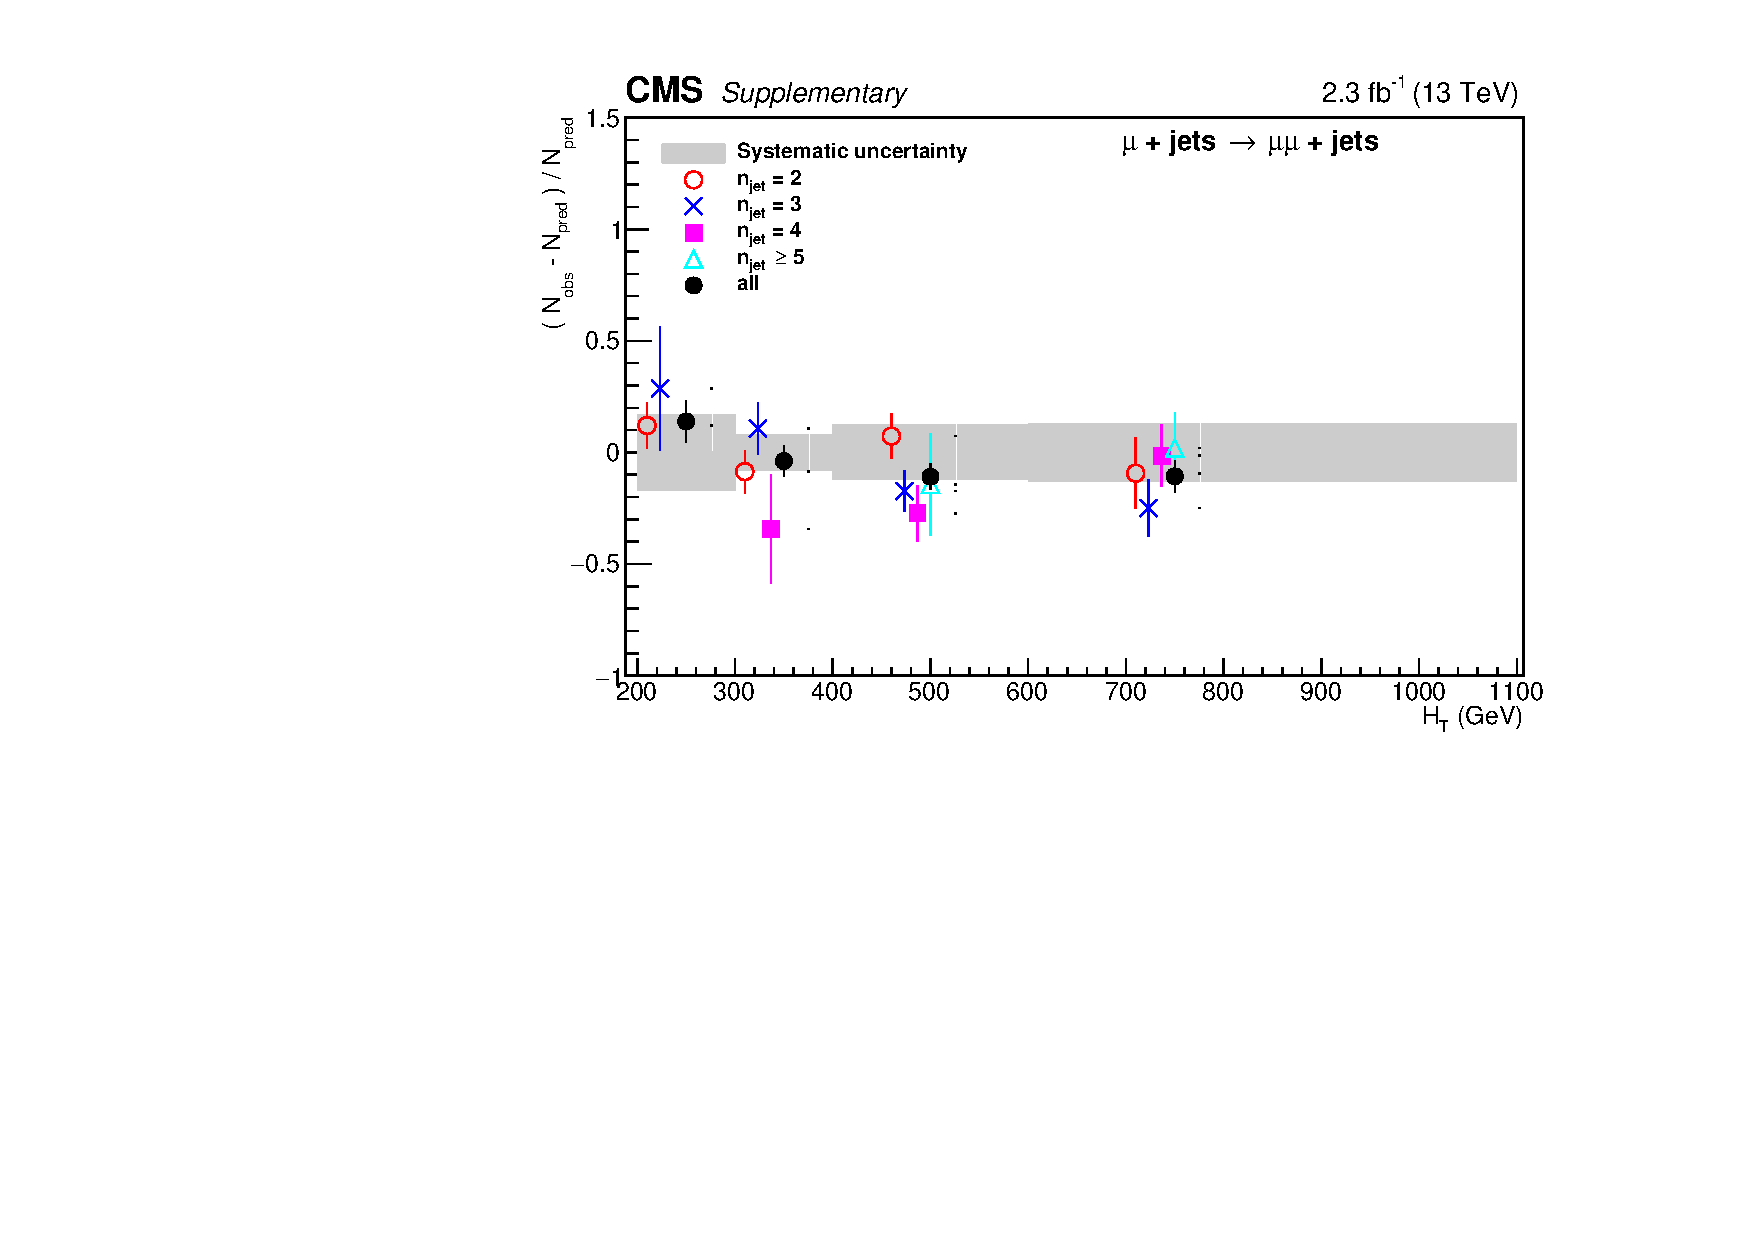
\includegraphics[width=0.48\textwidth]{figures/mu_mumusym_half_noFit} ~~
     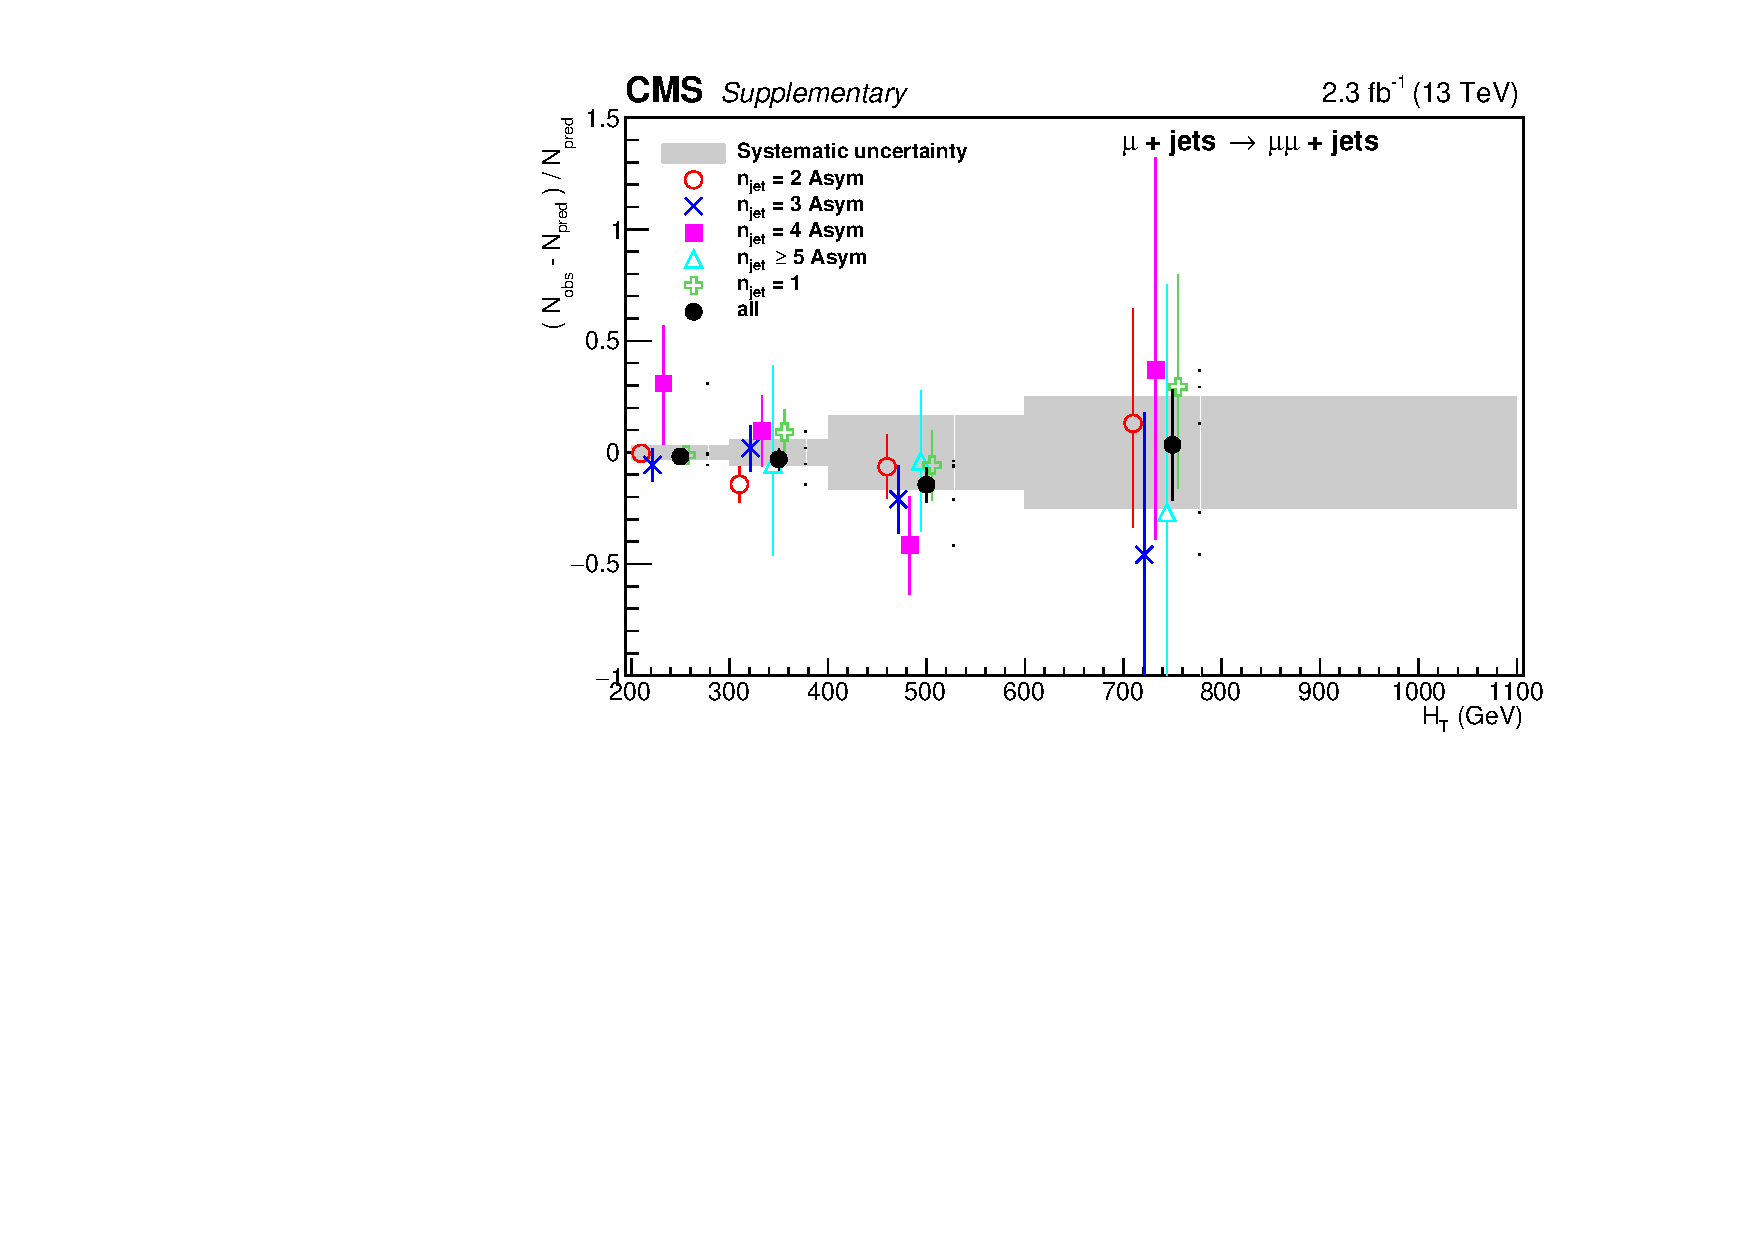
\includegraphics[width=0.48\textwidth]{figures/mu_mumuasym_half_noFit}
  \end{center}
\end{figure}





\clearpage
\begin{figure}[tbhp]
    \caption{ 
    Validation of the \mht modelling in the MC, in bins of (\nj,\nb,\scalht), for the $\gamma+\mathrm{jets}$ (top), $\mu+\mathrm{jets}$ (middle),             
    $\mu\mu+\mathrm{jets}$ (bottom) control regions. The data/MC ratio is fitted with constant and linear functions to spot for possible 
    trends and the result of these fits are shown in the plot. The best fit value of the linear function and its uncertainty are propagated 
    to assign shape systematic uncertainty in each (\nj,\nb,\scalht) category. 
    \label{fig:mht-validation} }
  \begin{center}
    \subfigure[$\gamma+\mathrm{jets}$, $\nj=2,\nb=0,600<\scalht<800 \, \mathrm{GeV}$]{ 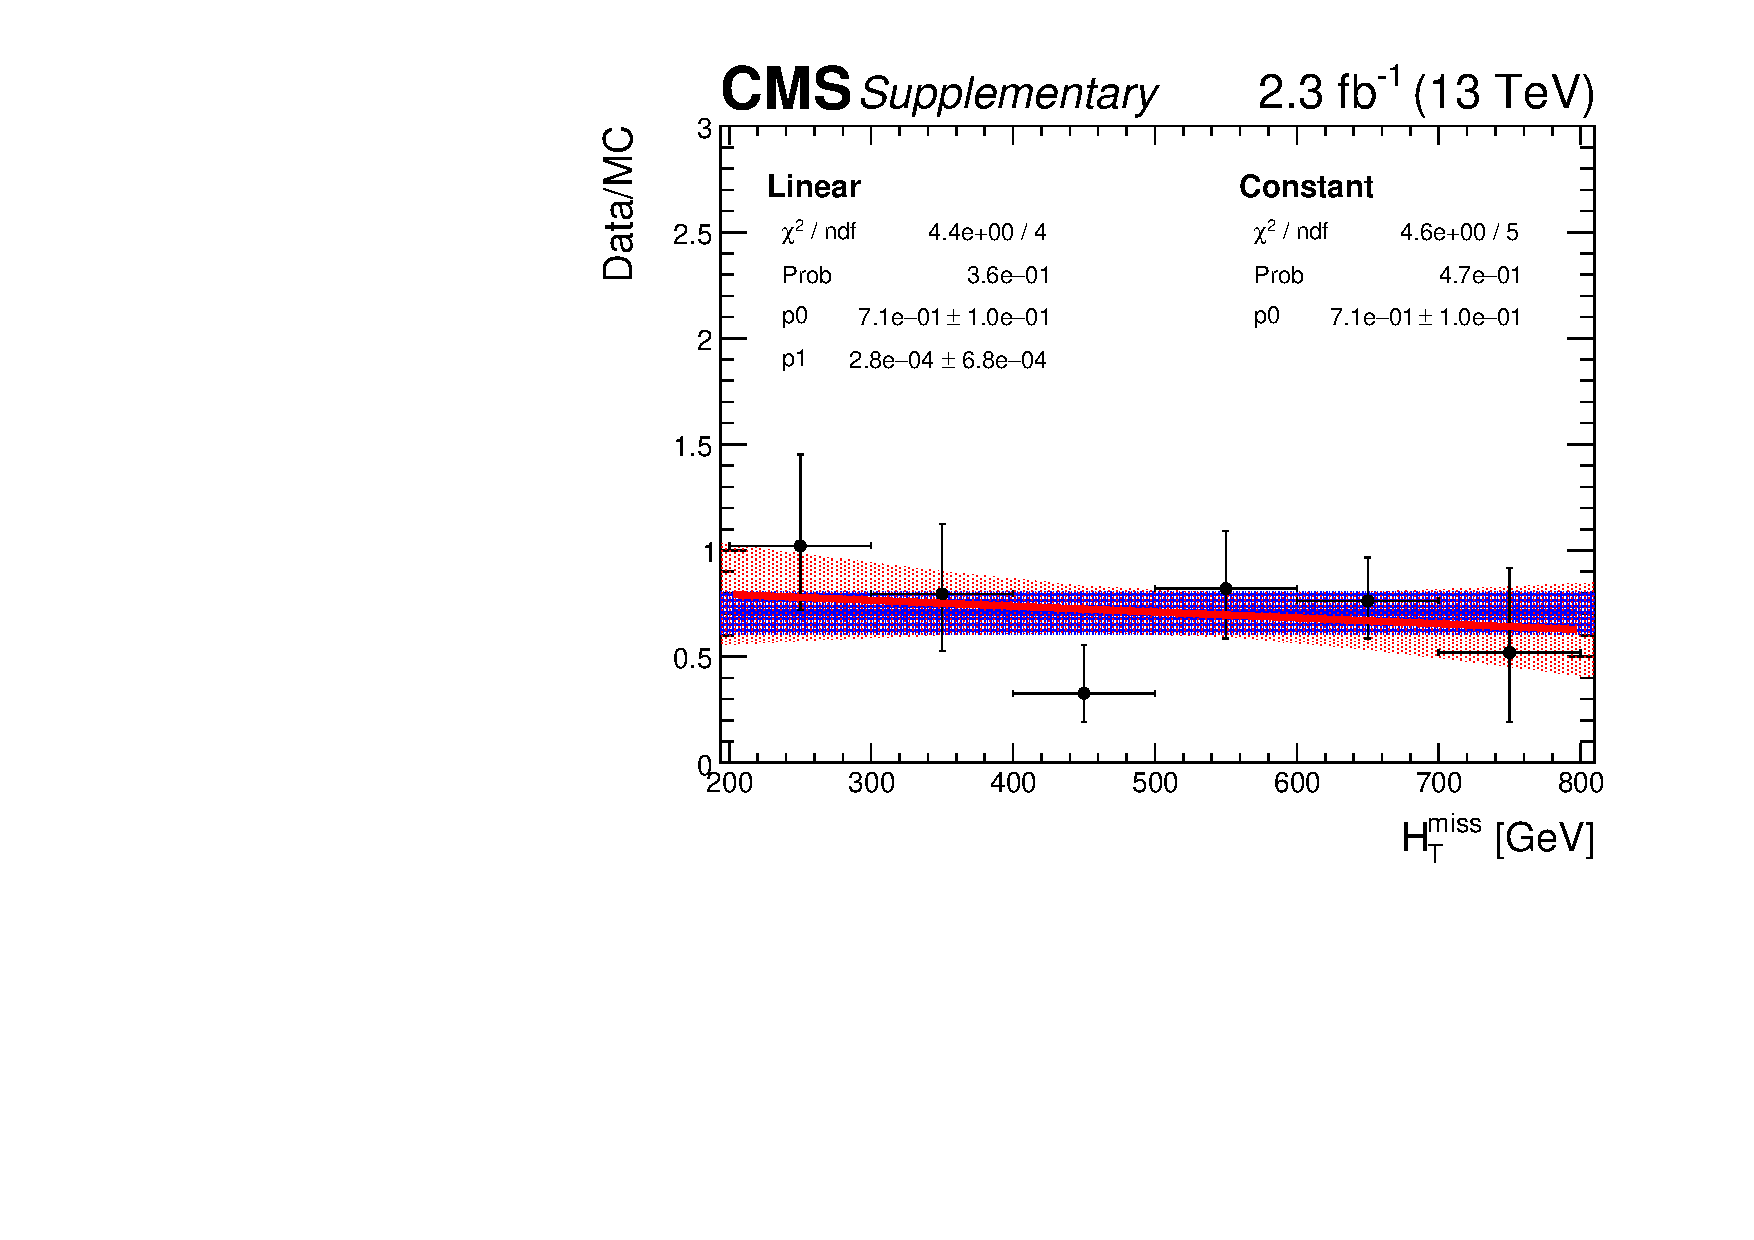
\includegraphics[width=0.45\textwidth]{figures/mht_eq0b_eq2j_ht_600_800_SinglePhoton_Graph} } ~~
    \subfigure[$\gamma+\mathrm{jets}$, $\nj=4,\nb=1,600<\scalht<800 \, \mathrm{GeV}$]{ 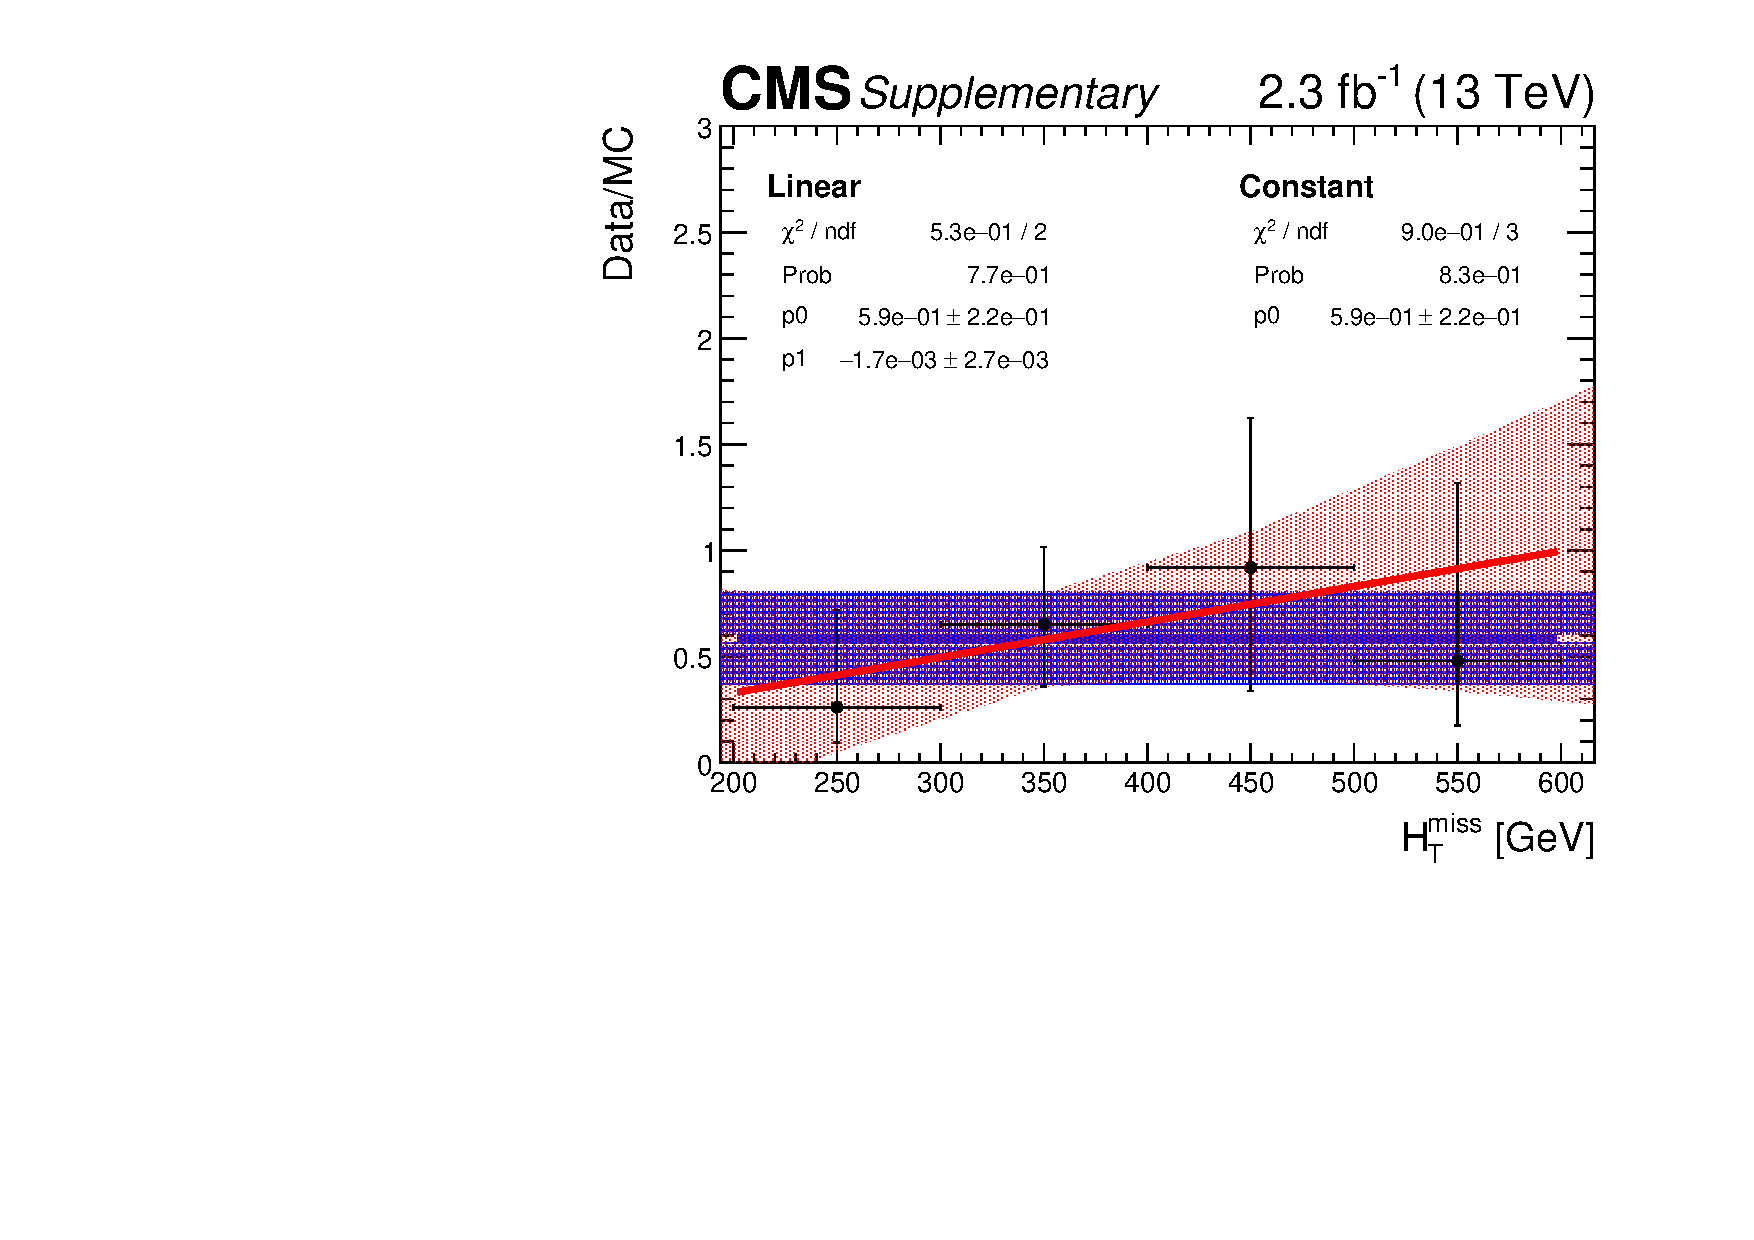
\includegraphics[width=0.45\textwidth]{figures/mht_eq1b_eq4j_ht_600_800_SinglePhoton_Graph} } \\
    \subfigure[$\mu+\mathrm{jets}$, $\nj^{asym}\geq5,\nb=2,350<\scalht<400 \, \mathrm{GeV}$]{ 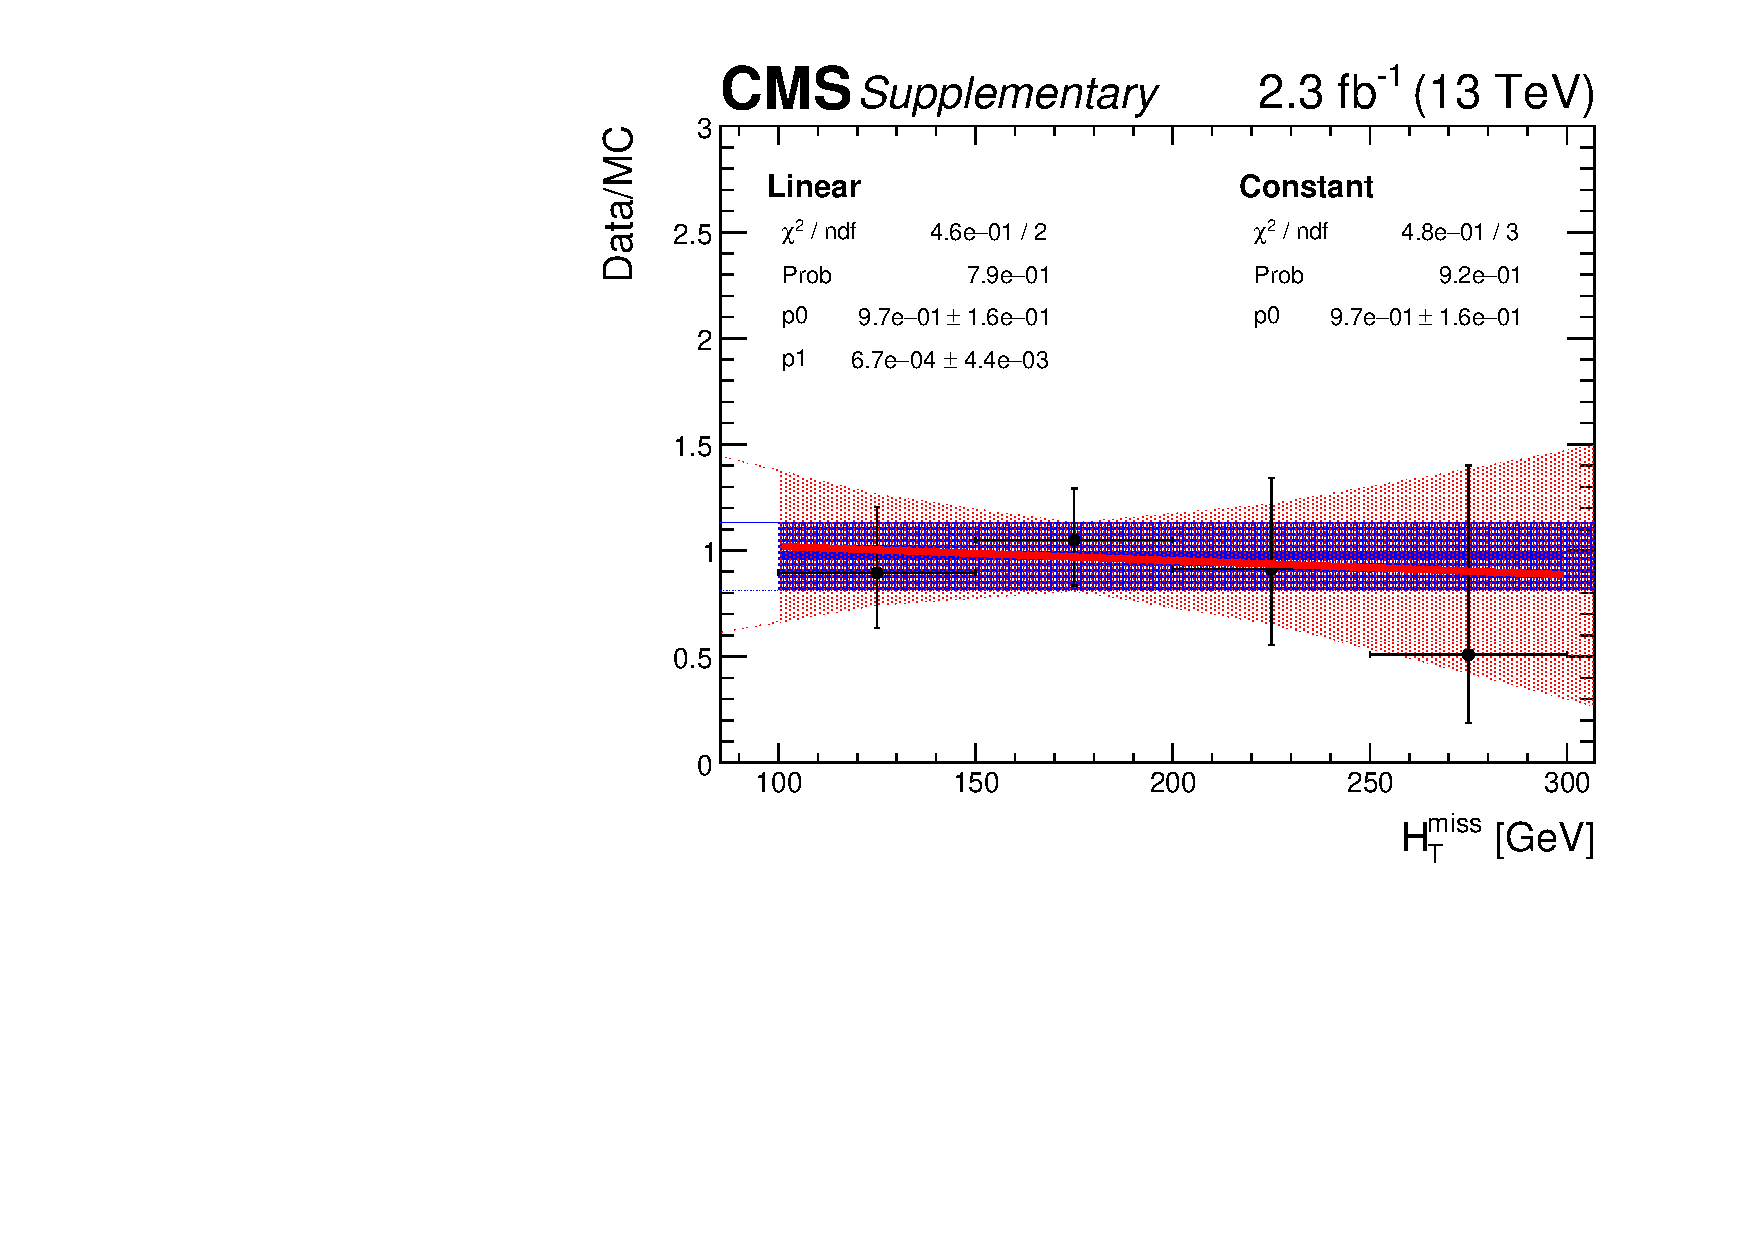
\includegraphics[width=0.45\textwidth]{figures/mht_eq2b_ge5a_ht_350_400_SingleMu_Graph} } ~~
    \subfigure[$\mu+\mathrm{jets}$, $\nj\geq5,\nb=0,\scalht>800 \, \mathrm{GeV}$]{ 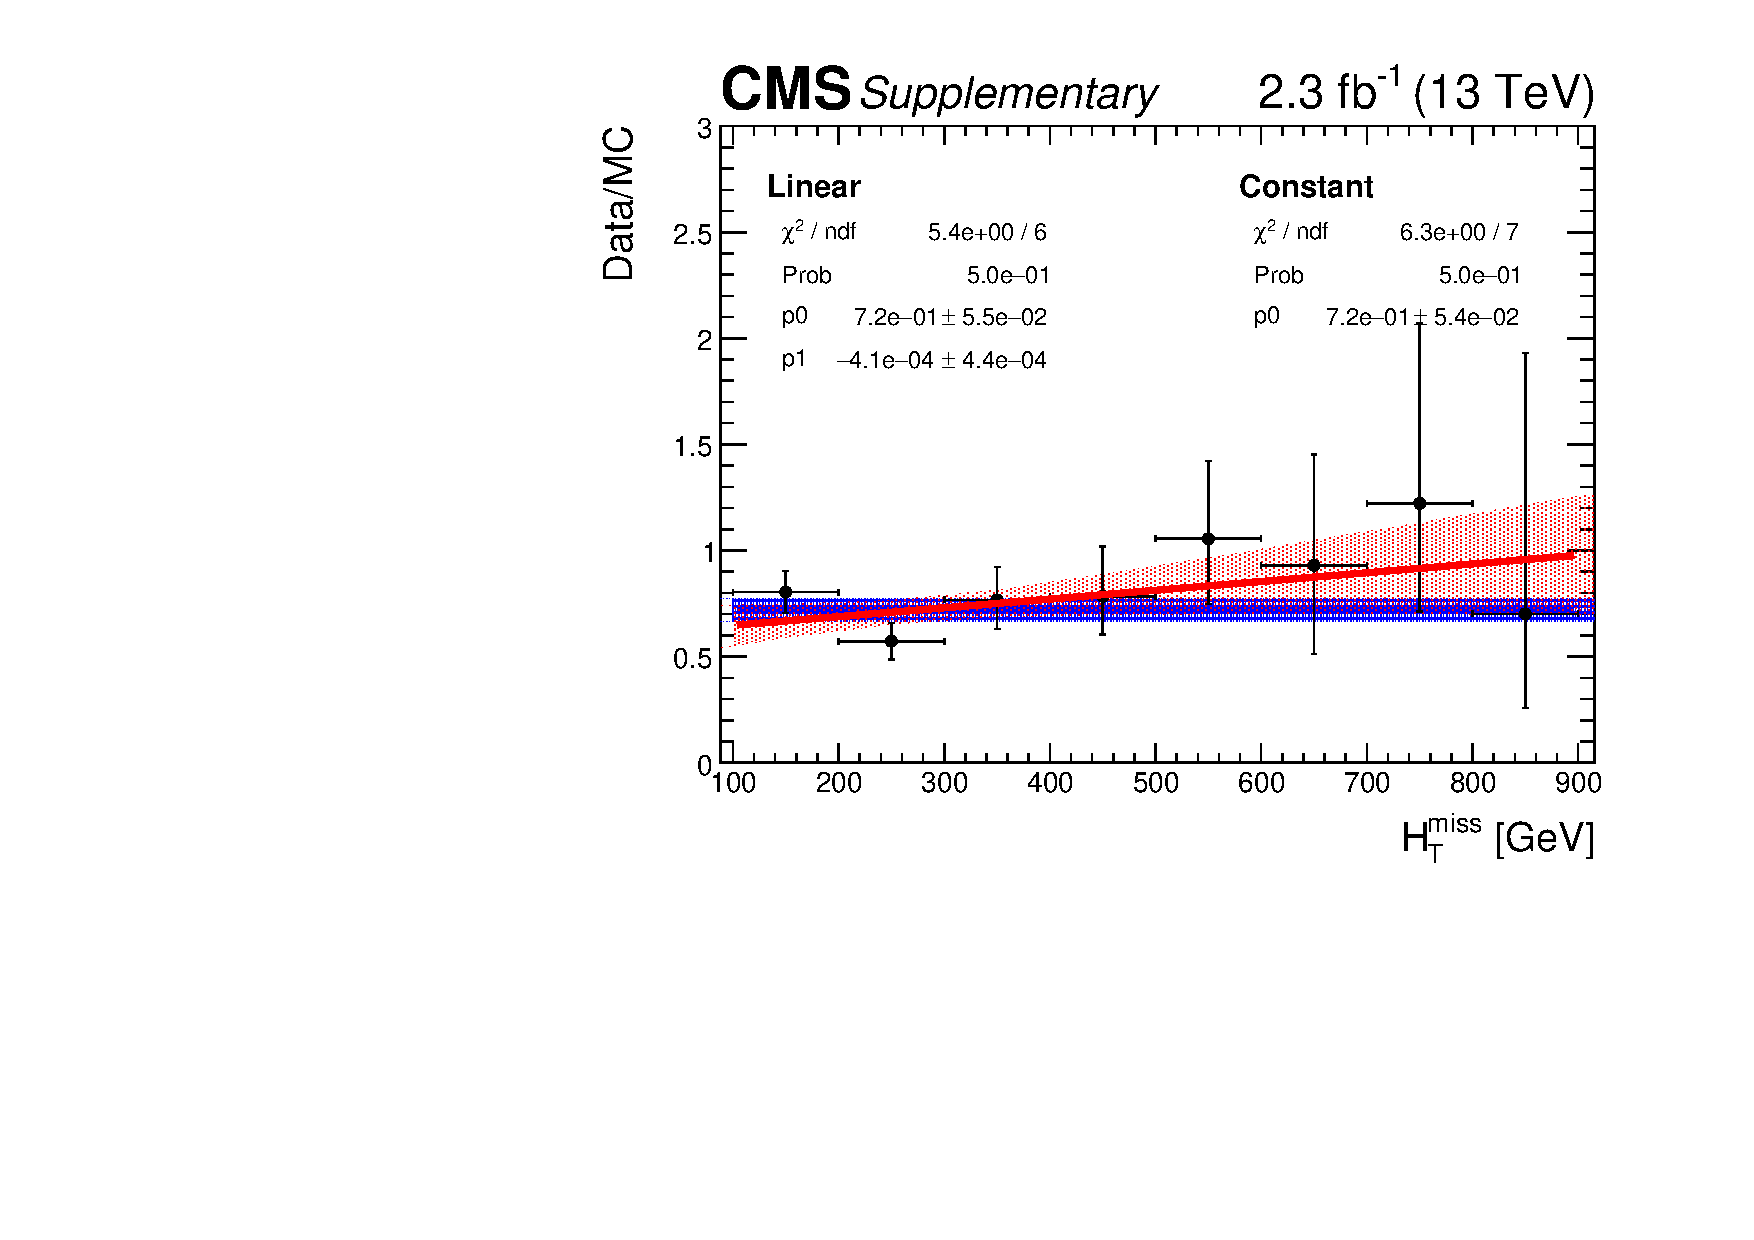
\includegraphics[width=0.45\textwidth]{figures/mht_eq0b_ge5j_ht_800_Inf_SingleMu_Graph} } \\
    \subfigure[$\mu\mu+\mathrm{jets}$, $\nj^{asym}=3,\nb=0,200<\scalht<250 \, \mathrm{GeV}$]{ 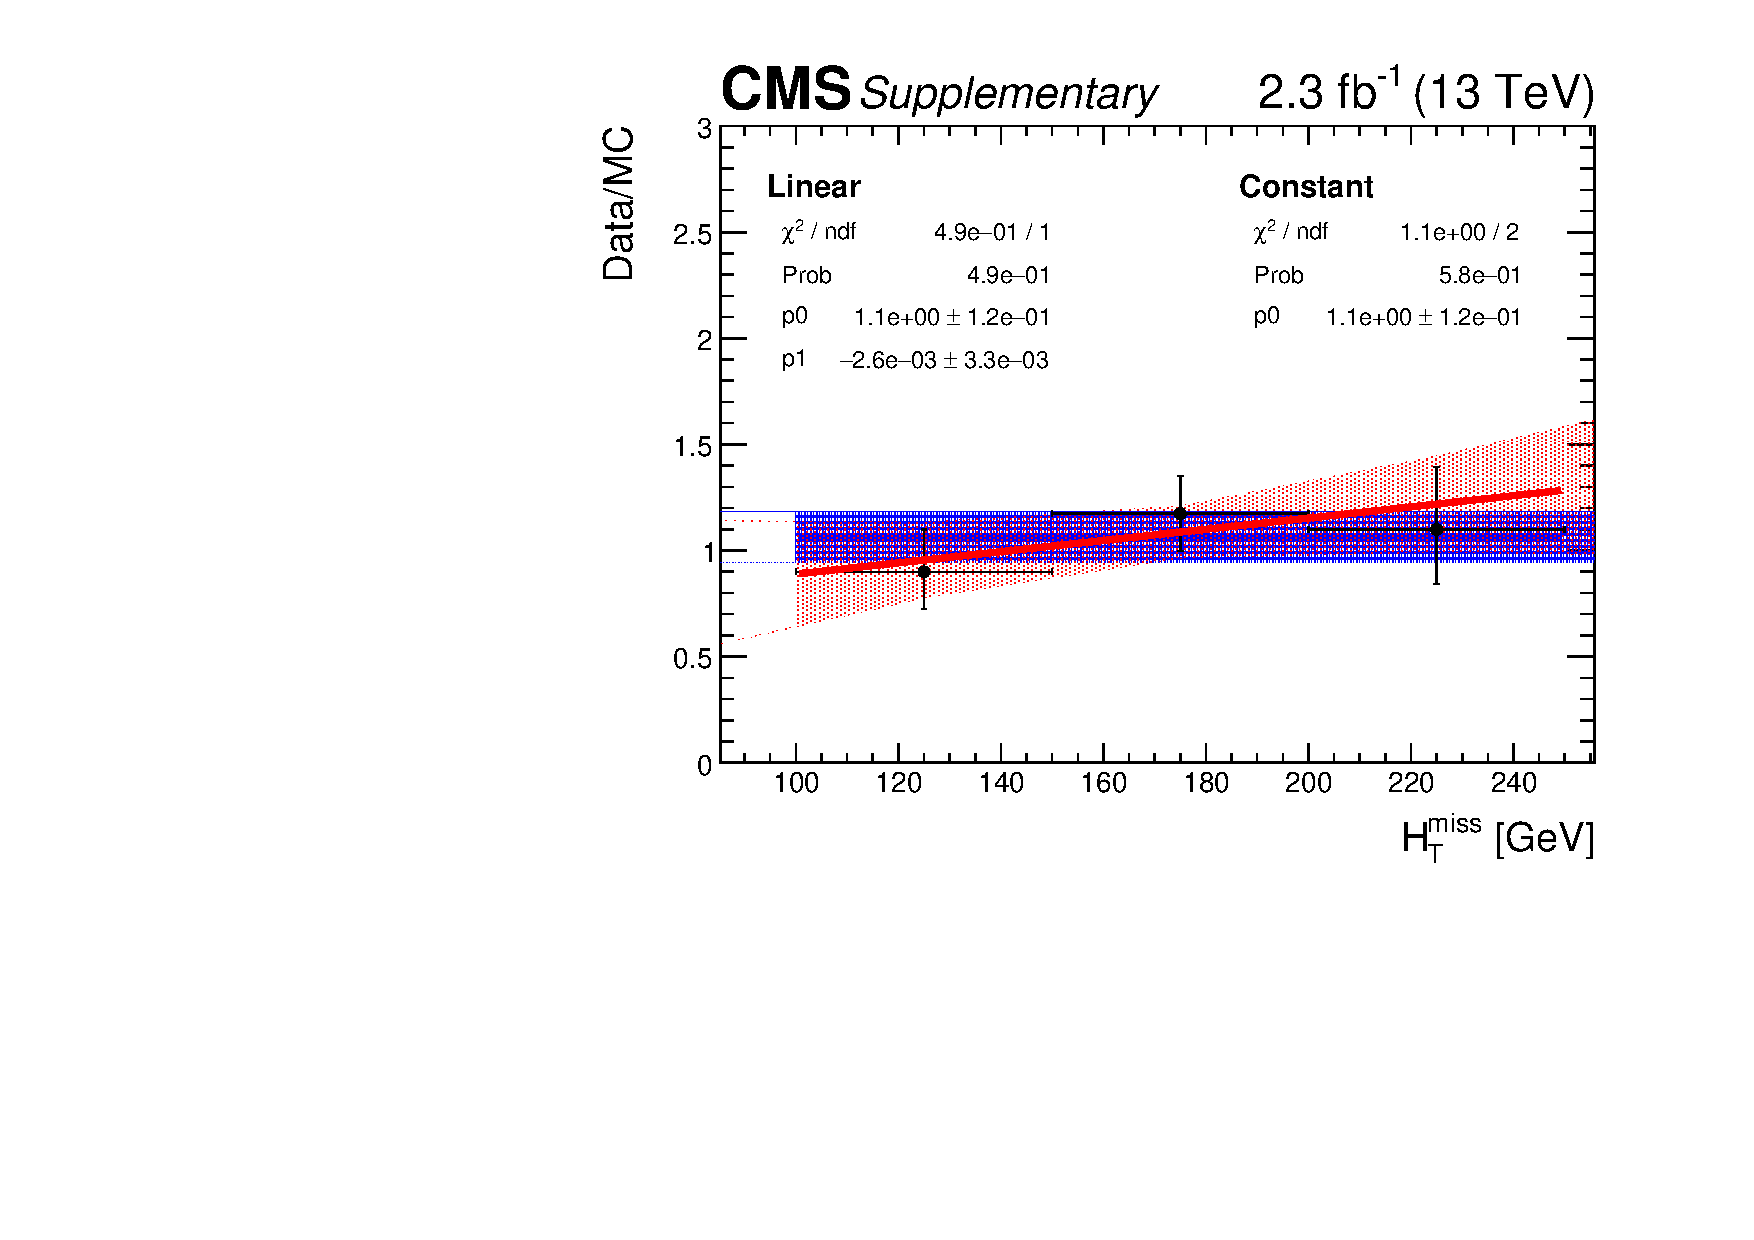
\includegraphics[width=0.45\textwidth]{figures/mht_eq0b_eq3a_ht_200_250_DoubleMu_Graph} } ~~
    \subfigure[$\mu\mu+\mathrm{jets}$, $\nj=2,\nb=0,400<\scalht<500 \, \mathrm{GeV}$]{ 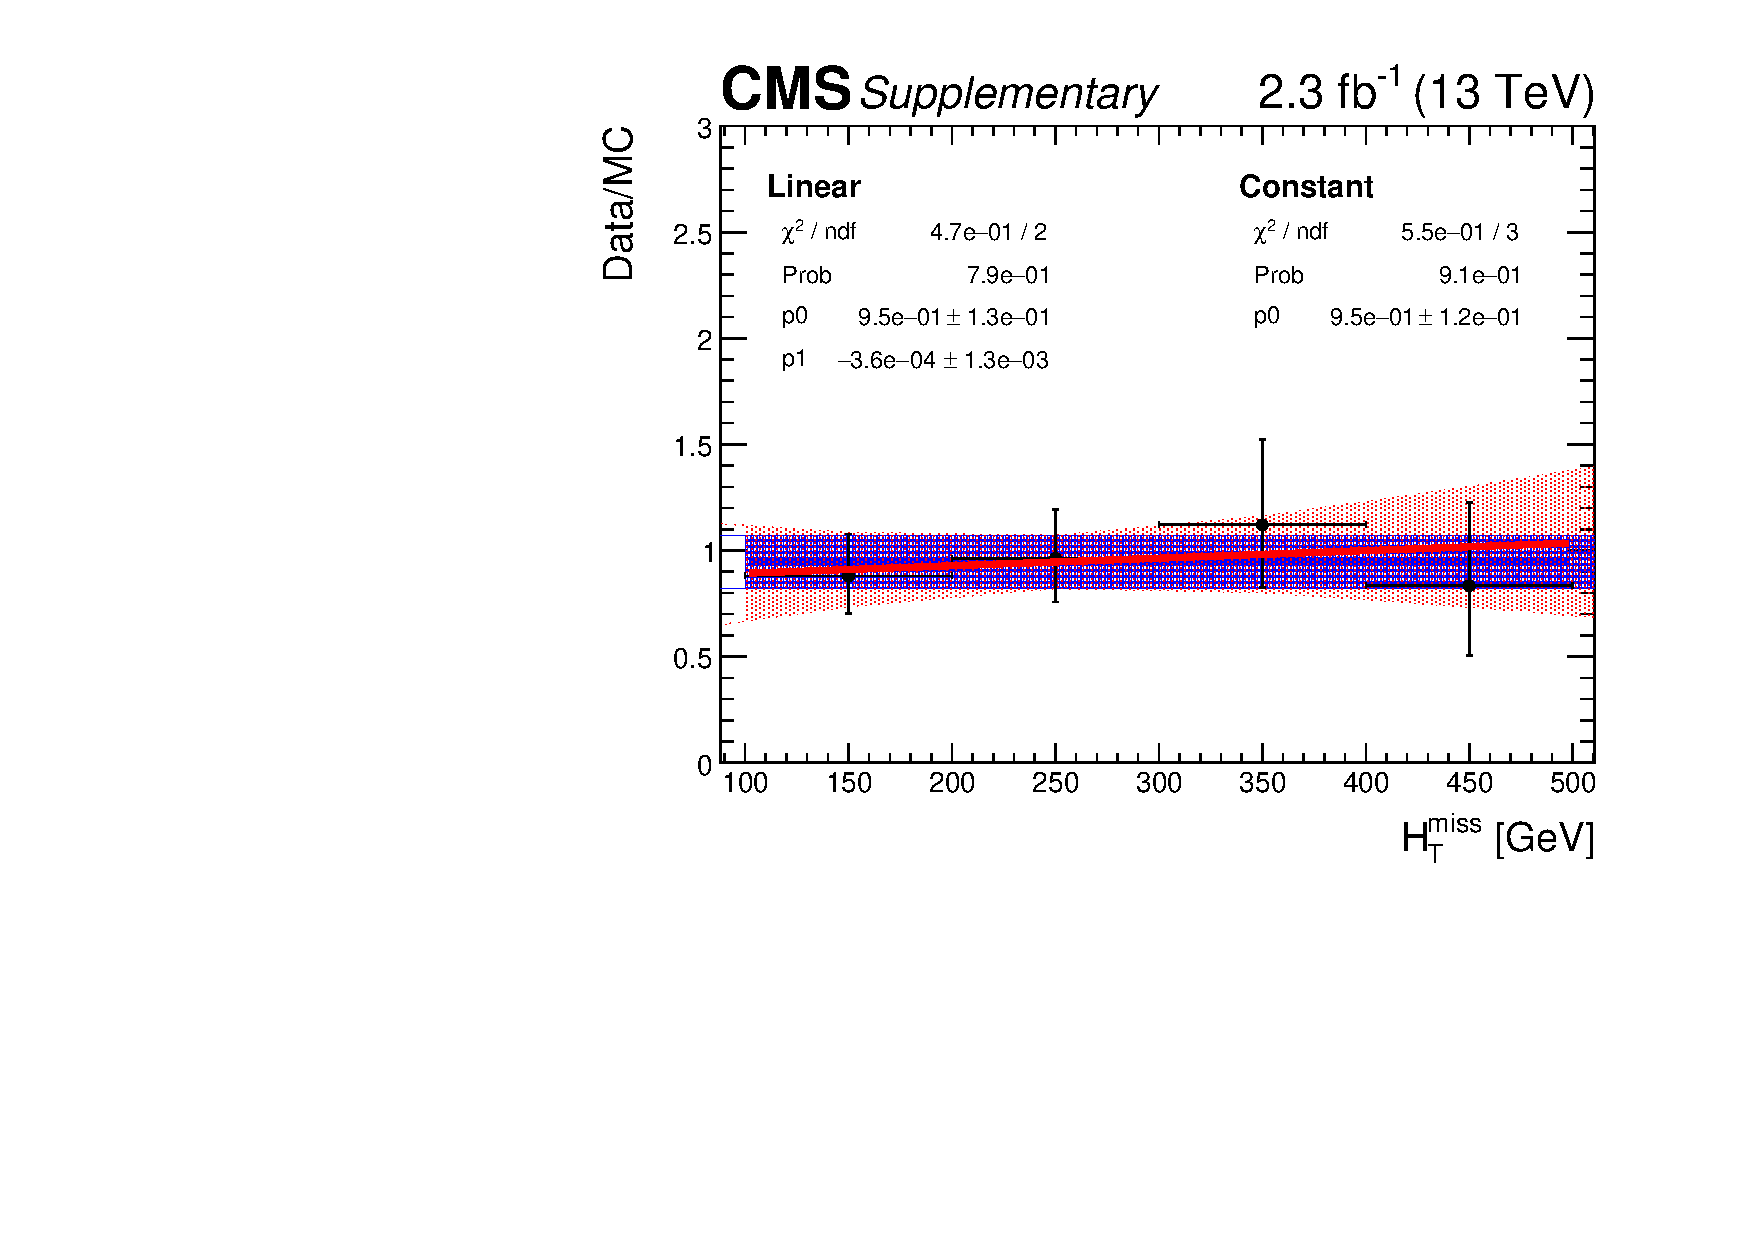
\includegraphics[width=0.45\textwidth]{figures/mht_eq0b_eq2j_ht_400_500_DoubleMu_Graph} } \\
  \end{center}
\end{figure}


\clearpage
\begin{landscape}
\begin{table}[h!]
  \caption{Summary of the systematics on the transfer factors considered in the analysis, 
    with representatives ranges of uncertainties and the correlation assumed, 
    for the predictions of the $\ttbar$, W and $\znunu$  background
    components.}
  \label{tab:systs}
  \centering
  \footnotesize
  \begin{tabular}{ ccccccc }
    \hline
    \hline
    Systematic & Method & \multicolumn{4}{c}{Relative uncertainty on transfer factor} & Correlation model \\    
     & & $\mj \rightarrow \znunu$  & $\mmj \rightarrow \znunu$ & $\gj \rightarrow \znunu$ & $\mj \rightarrow \ttbar+W$ & \\
    \hline
    \alphat/\bdphi extrapolation & data-driven tests & $5-80\%$ &
    $50-80\%$ & - & $5-80\%$ & un-correlated across \scalht/jet top. \\
    W/Z ratio & data-driven tests & $10-30\%$ & - & - & - & un-correlated across \scalht/jet top. \\
    Z/$\gamma$ ratio & data-driven tests & - & - & $10-30\%$ & - & un-correlated across \scalht/jet top. \\
    W/\ttbar admixture & data-driven tests & - & - & - & $10-100\%$ & un-correlated across \scalht/jet top. \\
    W polarisation & data-driven tests & $5-50\%$ & - & - & $5-50\%$ & un-correlated across \scalht/jet top. \\
    Jet energy scale & MC variations & $<15\%$ & $<10\%$ & $<15\%$ &
    $<15\%$ & fully correlated \\
    B-tagging efficiency & MC variations & $<5\%$ & $<2\%$ & $<2\%$
    & $<5\%$ & fully correlated \\
    Pileup weights & MC variations & $<6\%$ & $<4\%$ & $<3\%$ & $<10\%$ & fully correlated \\
    Top $p_{T}$ weights & MC variations & $<20\%$  & $<4\%$ & - &
    $<5\%$ & fully correlated \\
    Lepton selection & MC variations & - & - & - & $2-5\%$ & fully correlated \\
    \hline
    \hline
  \end{tabular}
\end{table}

\end{landscape}


\clearpage
\begin{landscape}
  \begin{center}
    \begin{figure*}[h!]
      \caption{Top: background yield predictions and data observation for the (\njet,\nb,\scalht) analysis bins (integrated over \mht) in the ``monojet'' search regions. Some benchmark signal models of gluino pair production are also shown, corresponding to ``compressed'' and ``uncompressed'' scenarios. Bottom: pre-fit and post-fit normalised pulls, defined as $(\mathrm{data}-\mathrm{SM total})/\sigma_{bkg}$, where $\sigma_{bkg}=\sqrt{\sigma^{2}_{syst.}+\sigma^{2}_{stat.}}$.  \label{fig:summaryPlot_Monojet}}.
      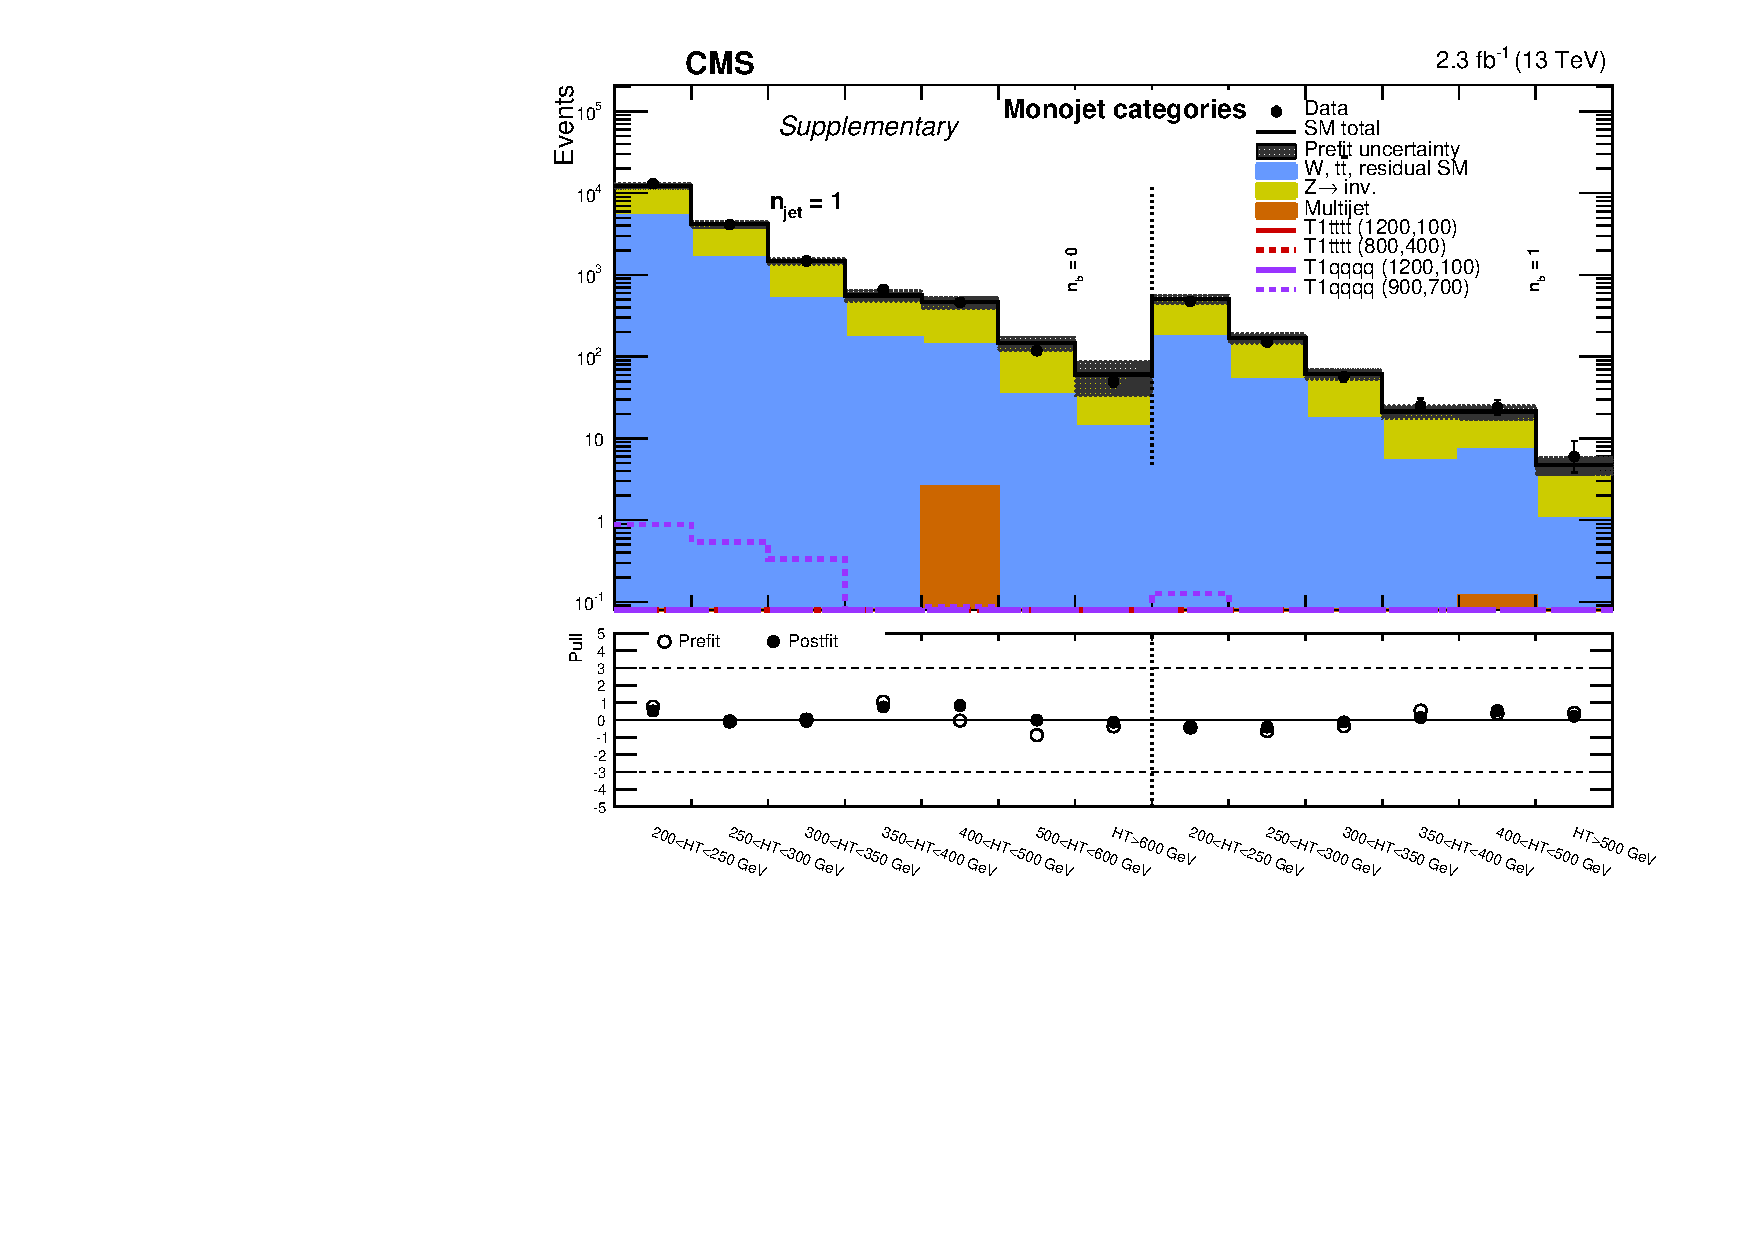
\includegraphics[width=0.75\linewidth]{supplementary/figures/summaryPlot_Monojet_prefit_overlay_fit_b}
    \end{figure*}
  \end{center}
\end{landscape}

\clearpage
\begin{landscape}
  \begin{center}
    \begin{figure*}[h!]
      \caption{Top: background yield predictions and data observation for the (\njet,\nb,\scalht) analysis bins (integrated over \mht) in the ``asymmetric'' search regions. Some benchmark signal models of gluino pair production are also shown, corresponding to ``compressed'' and ``uncompressed'' scenarios. Bottom: pre-fit and post-fit normalised pulls, defined as $(\mathrm{data}-\mathrm{SM total})/\sigma_{bkg}$, where $\sigma_{bkg}=\sqrt{\sigma^{2}_{syst.}+\sigma^{2}_{stat.}}$. \label{fig:summaryPlot_Asymmetric}}.
      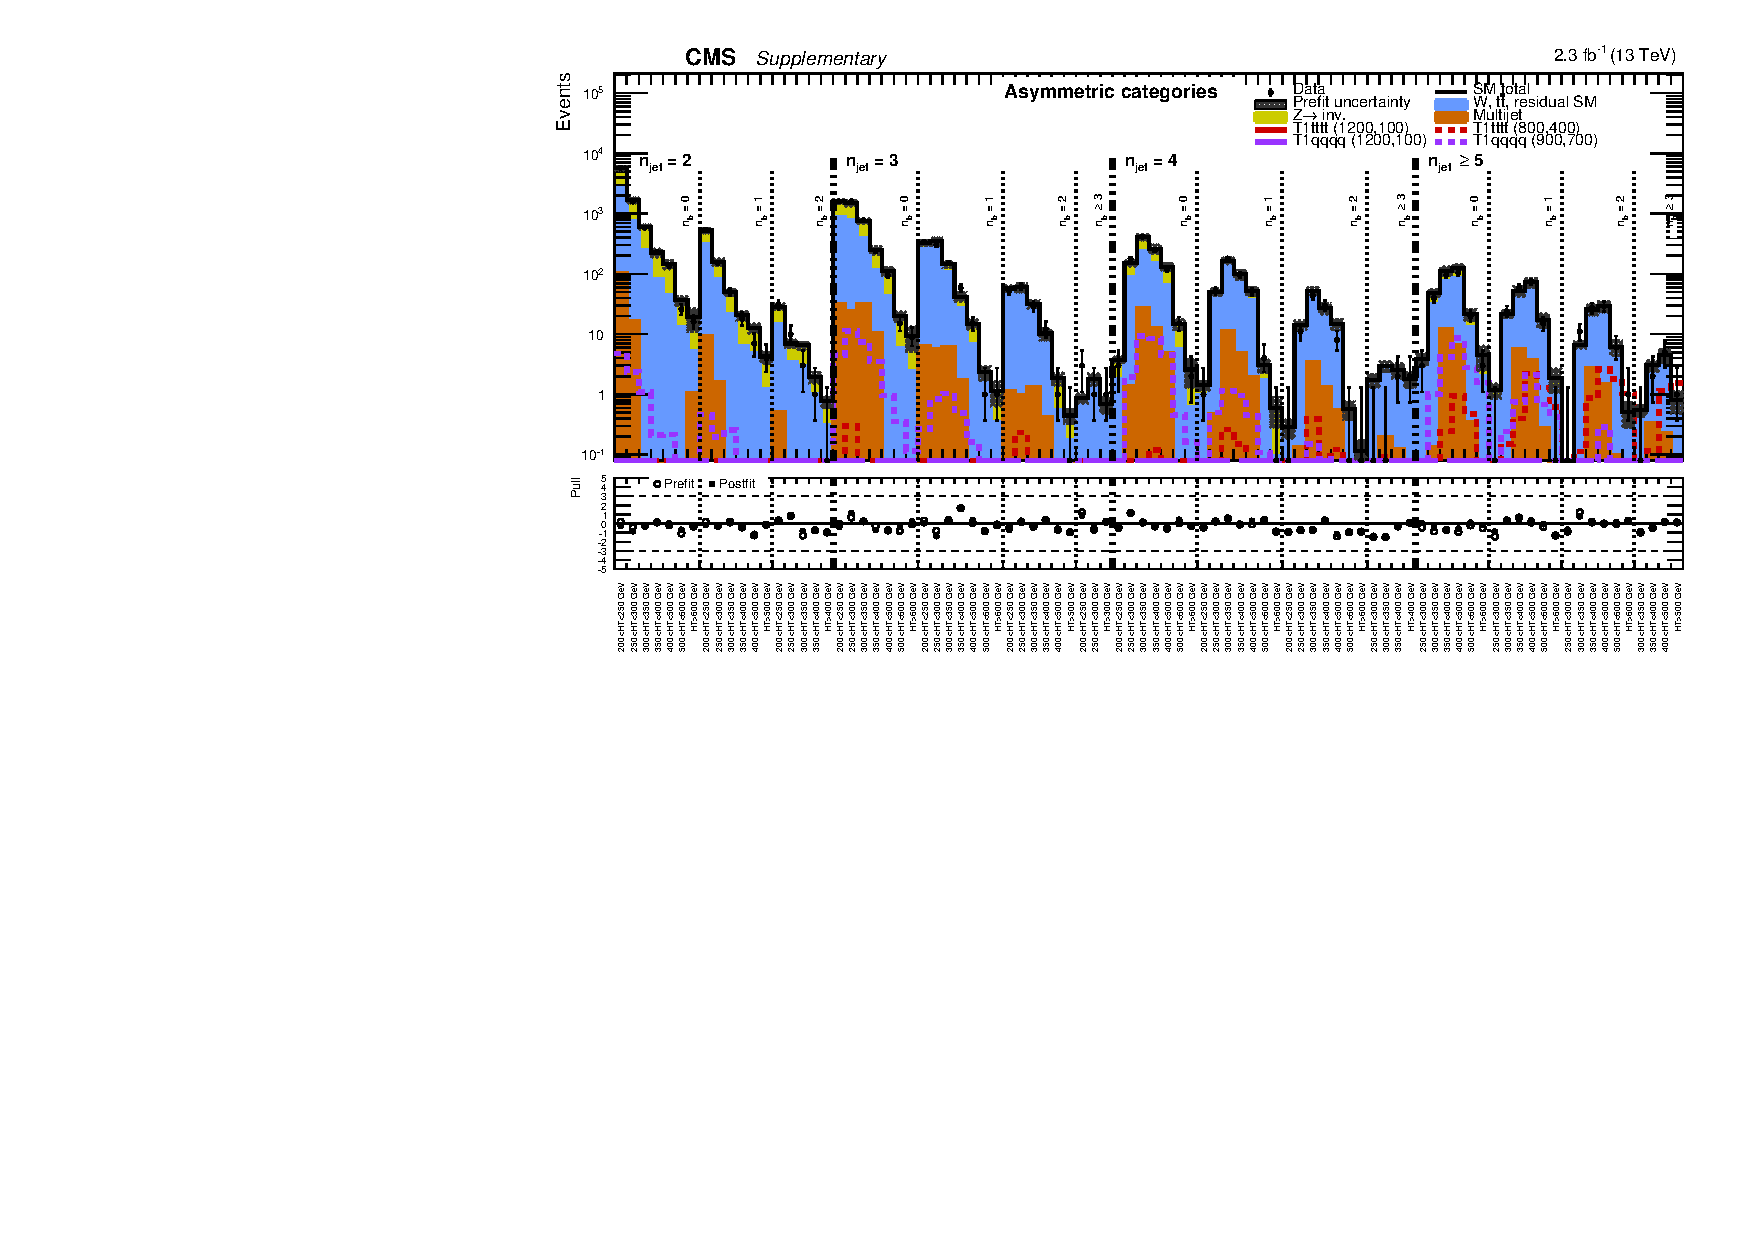
\includegraphics[width=0.8\linewidth]{supplementary/figures/summaryPlot_Asymmetric_prefit_overlay_fit_b}
    \end{figure*}
  \end{center}
\end{landscape}

\clearpage
\begin{landscape}
  \begin{center}
    \begin{figure*}[h!]
      \caption{Top: background yield predictions and data observation for the (\njet,\nb,\scalht) analysis bins (integrated over \mht) in the ``symmetric'' search regions. Some benchmark signal models of gluino pair production are also shown, corresponding to ``compressed'' and ``uncompressed'' scenarios. Bottom: pre-fit and post-fit normalised pulls, defined as $(\mathrm{data}-\mathrm{SM total})/\sigma_{bkg}$, where $\sigma_{bkg}=\sqrt{\sigma^{2}_{syst.}+\sigma^{2}_{stat.}}$. \label{fig:summaryPlot_Symmetric}}.
      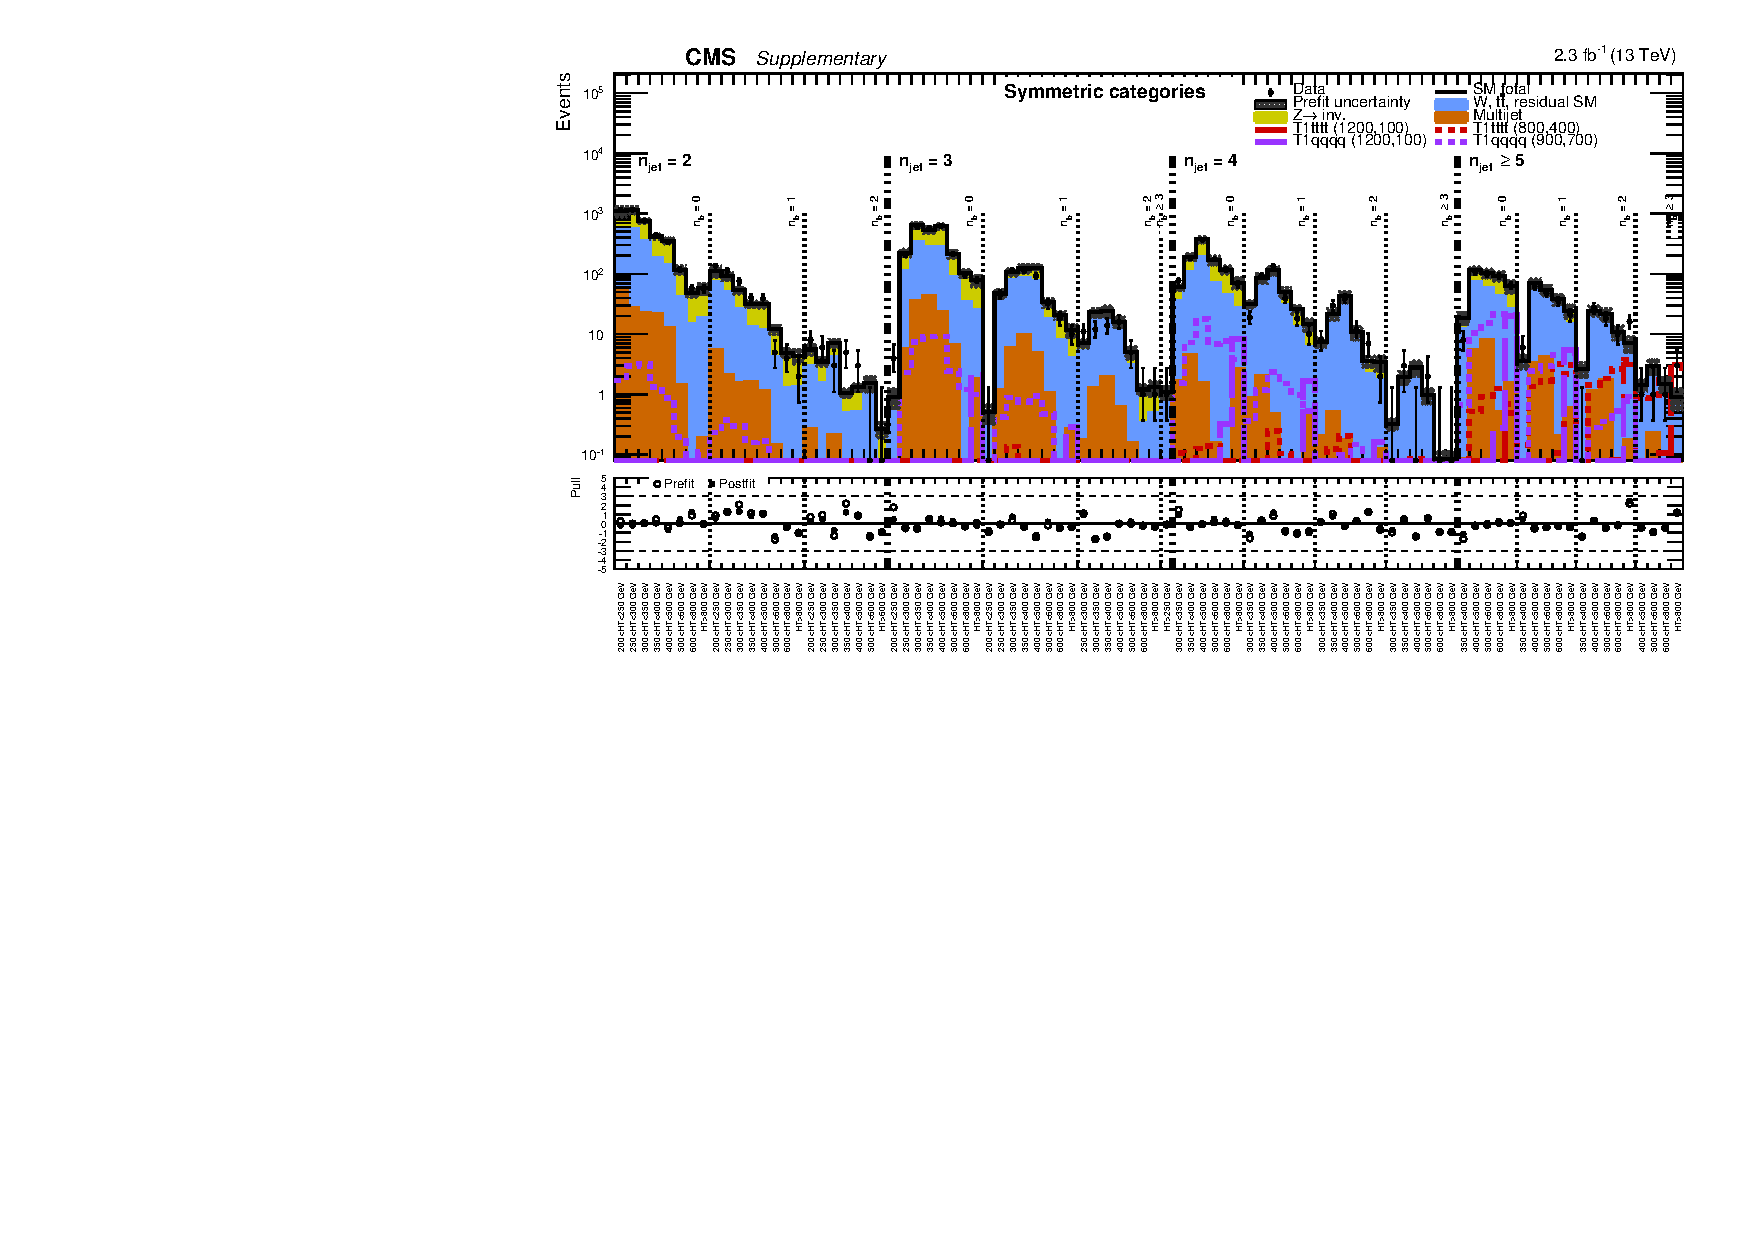
\includegraphics[width=0.8\linewidth]{supplementary/figures/summaryPlot_Symmetric_prefit_overlay_fit_b}
    \end{figure*}
  \end{center}
\end{landscape}


\clearpage
\begin{figure}[tbhp]
    \caption{ \mht templates for some (\njet,\nb,\scalht) analysis bins. Benchmark models are also shown in the stack. \label{fig:mht-templates} }
  \begin{center}
    \subfigure[$\njet \geq 5$, $\nb \geq 3$, $\scalht > 800$ GeV]{ 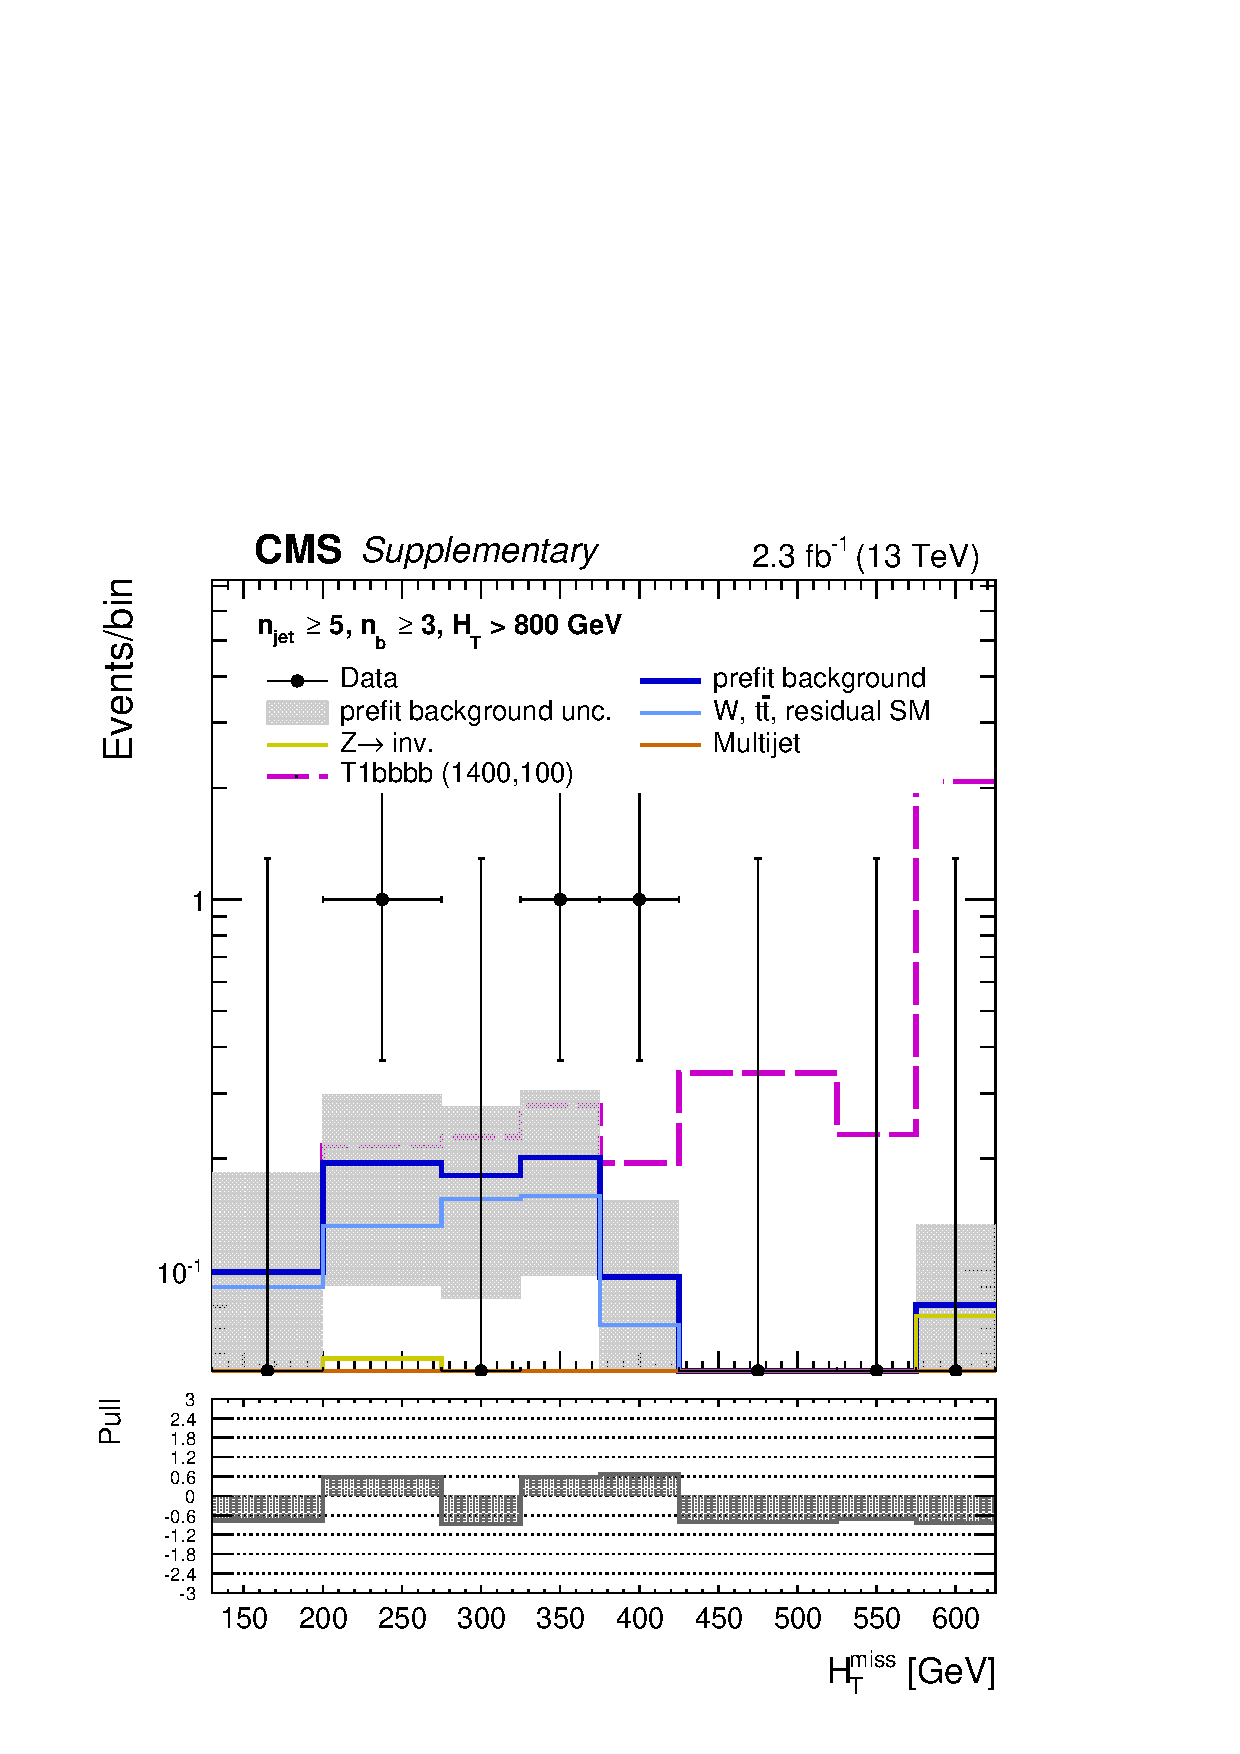
\includegraphics[width=0.45\textwidth]{figures/postFitShape_ge3b_ge5j_800_Inf_prefit_T1bbbb_1400_100} } ~~
    \subfigure[$\njet \geq 5$, $\nb = 0$, $600 < \scalht < 800$ GeV]{ 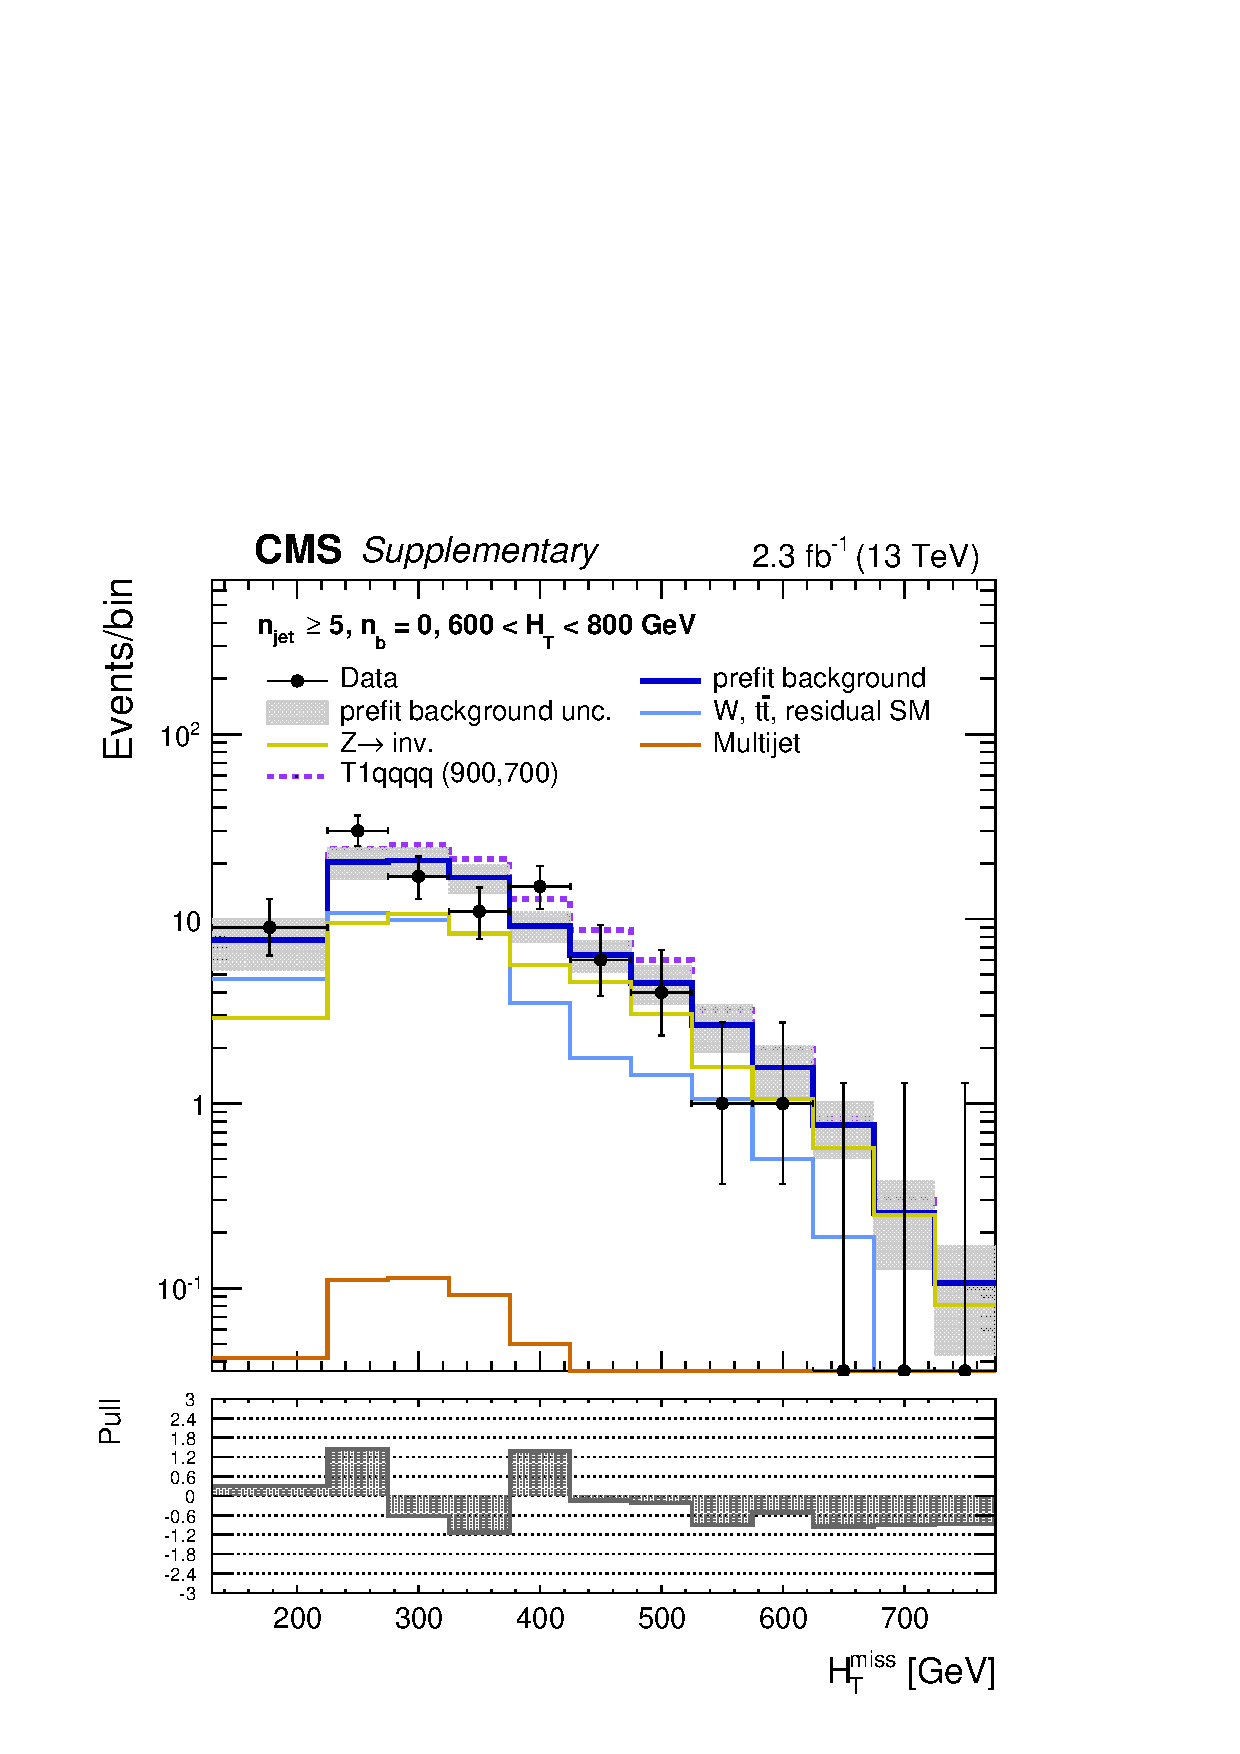
\includegraphics[width=0.45\textwidth]{figures/postFitShape_eq0b_ge5j_600_800_prefit_T1qqqq_900_700} } \\
    \subfigure[$\njet \geq 5$, $\nb = 1$, $\scalht > 800$ GeV]   { 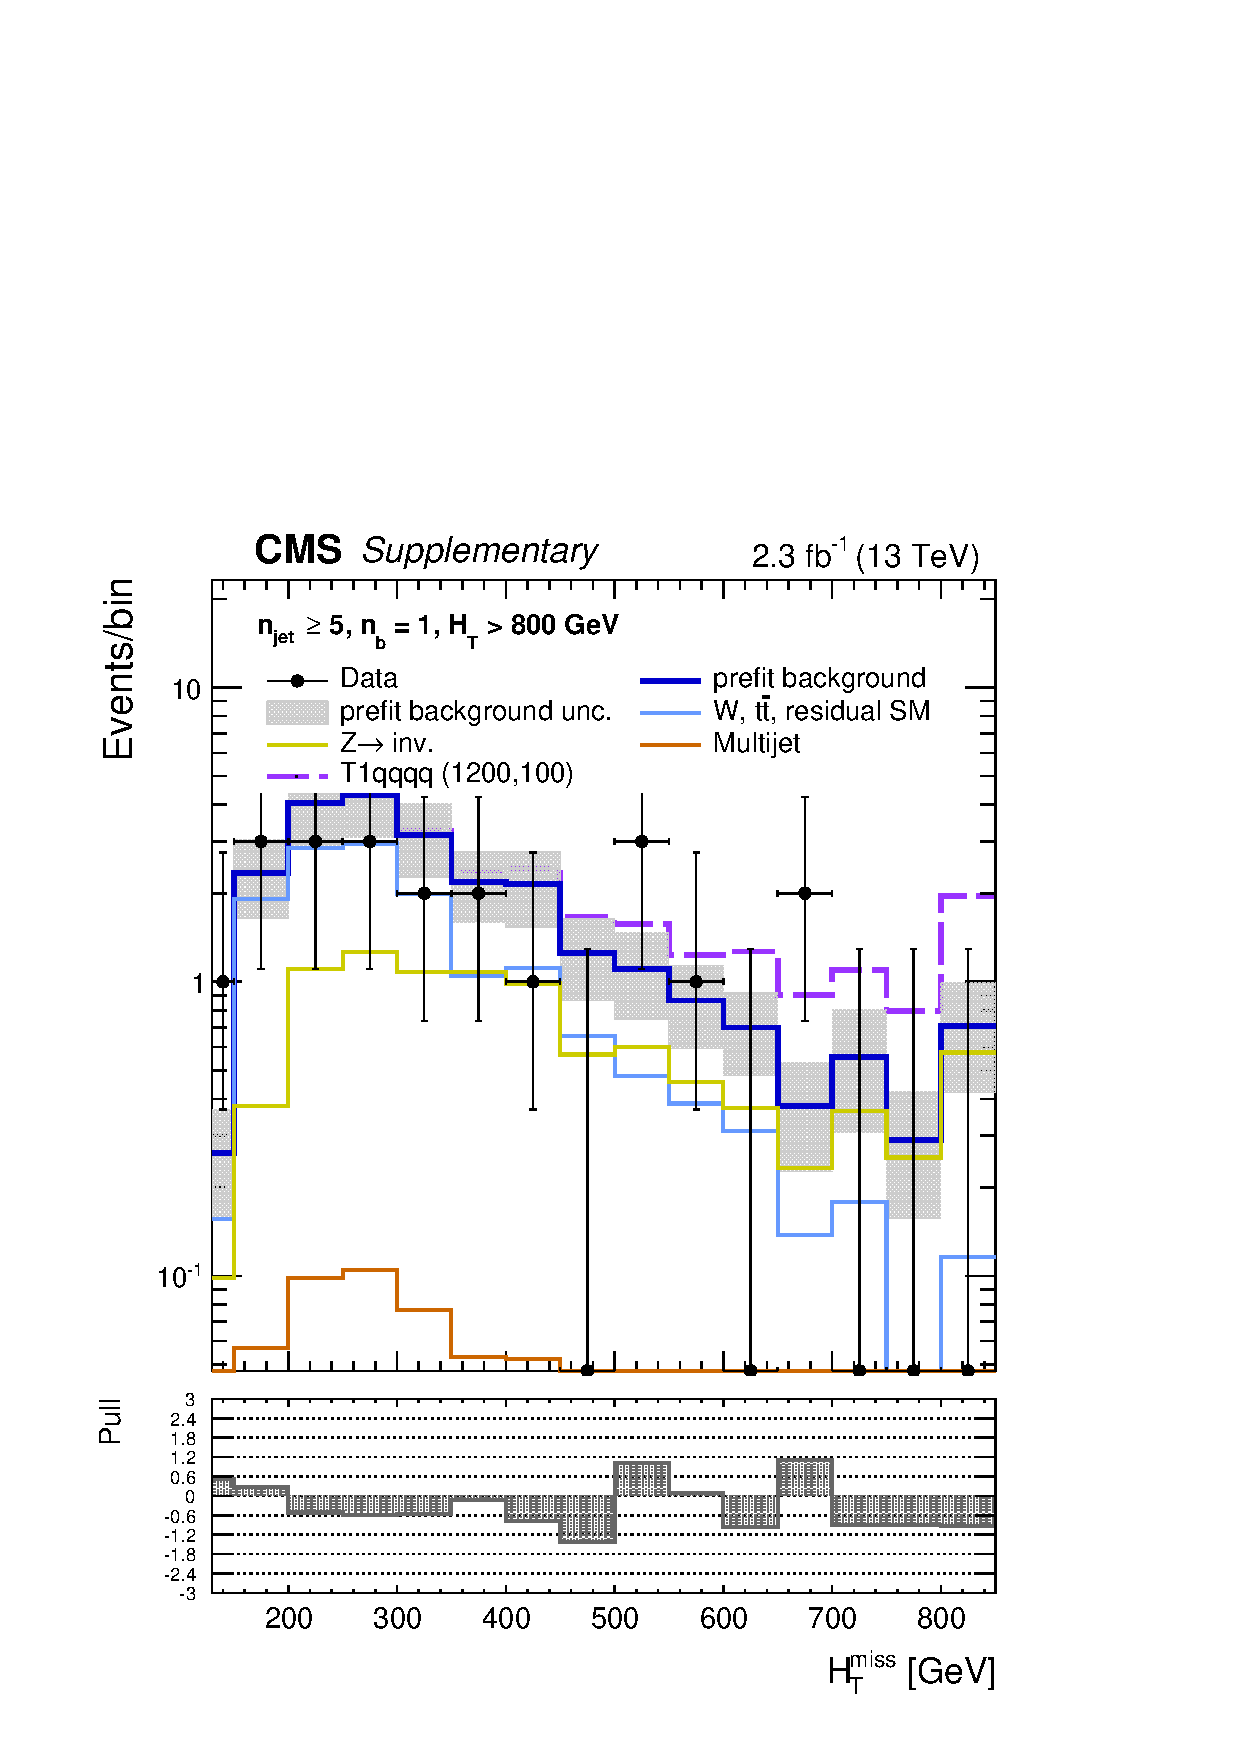
\includegraphics[width=0.45\textwidth]{figures/postFitShape_eq1b_ge5j_800_Inf_prefit_T1qqqq_1200_100} } ~~
    \subfigure[$\njet \geq 5$, $\nb = 2$, $\scalht > 800$ GeV]{ 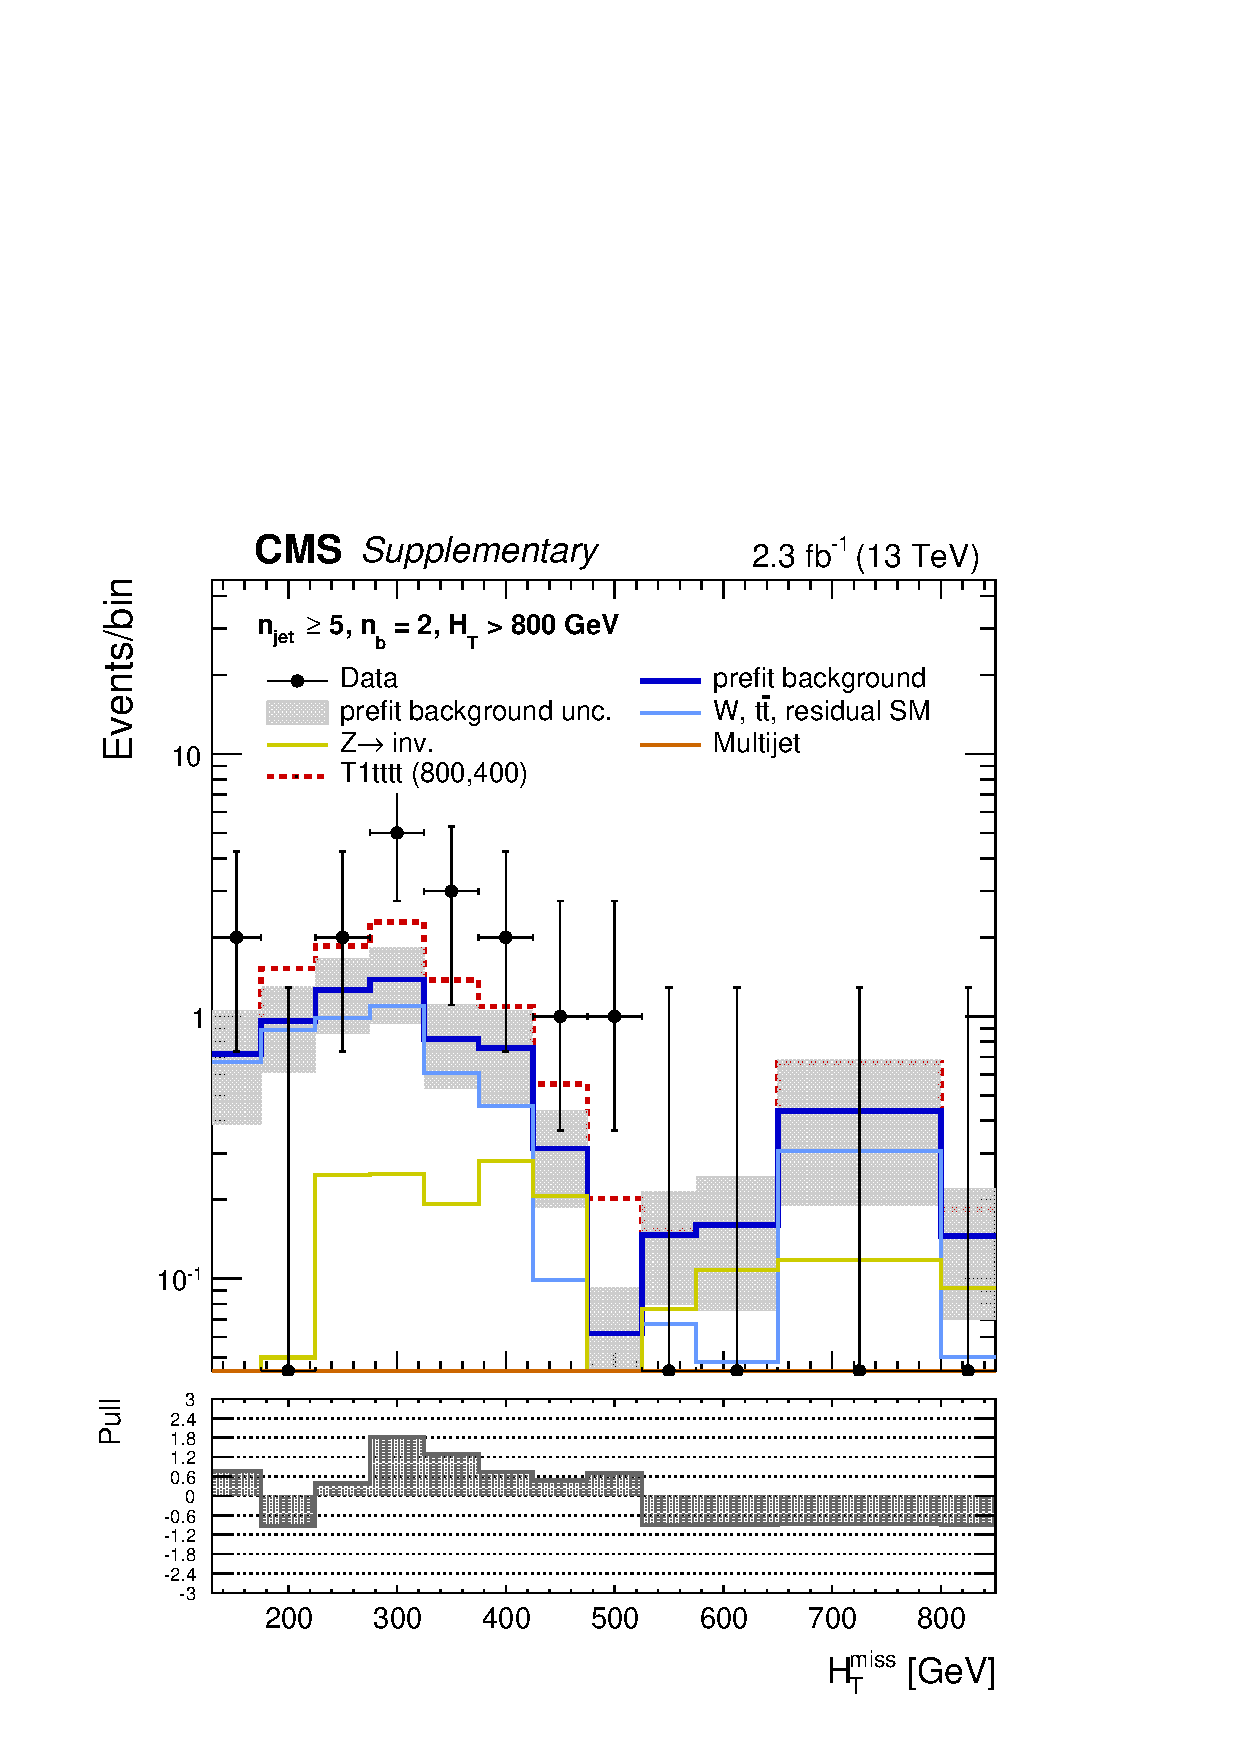
\includegraphics[width=0.45\textwidth]{figures/postFitShape_eq2b_ge5j_800_Inf_prefit_T1tttt_800_400} } \\
  \end{center}
\end{figure}



\clearpage
\begin{table}[h!]
  \caption{Representative range of uncertainty across the analysis bins 
    for each source of systematic uncertainty on the signal acceptance.
    Two benchmark points are chosen for each model, 
    corresponding to ``compressed'' and ``uncompressed'' scenarios, 
    i.e. with small and large mass splitting between the mother particle and the LSP.
    \label{tab:sig-systematics}   
  }
  \centering
  \begin{tabular}{ ccccccccc }
    \hline
    \hline
Model & ($m_{\mathrm{Susy}},m_{\mathrm{LSP}}$) & Luminosity & ISR & JEC & PU & b-tag & Trigger & MC stat. \\ \hline
\multirow{2}{*}{T1bbbb}
 & (1500,100) & 4.6\% & 1-2\% & 1-12\% & 1-4\% & 2-22\% & 1-3\% & 5-17\% \\ 
 & (1000,800) & 4.6\% & 1-17\% & 1-40\% & 1-20\% & 1-14\% & 1-15\% & 8-31\% \\ \hline 
\multirow{2}{*}{T1tttt}
 & (1300,100) & 4.6\% & 1-2\% & 2-7\% & 1-4\% & 2-12\% & 1-3\% & 7-16\% \\ 
 & (800,400) & 4.6\% & 1-2\% & 3-45\% & 1-13\% & 1-8\% & 1-10\% & 7-27\% \\ \hline 
\multirow{2}{*}{T1ttbb}
 & (1300,100) & 4.6\% & 1-2\% & 3-16\% & 1-18\% & 2-19\% & 1-4\% & 9-32\% \\ 
 & (1000,700) & 4.6\% & 1-9\% & 3-65\% & 1-12\% & 1-14\% & 1-14\% & 9-30\% \\ \hline 
\multirow{2}{*}{T5ttcc}
 & (1200,200) & 4.6\% & 5-25\% & 3-21\% & 1-9\% & 1-24\% & 2-6\% & 6-25\% \\ 
 & (750,600) & 4.6\% & 1-4\% & 5-21\% & 1-8\% & 1-3\% & 4-7\% & 9-23\% \\ \hline 
\multirow{2}{*}{T5ttttDM175}
 & (800,100) & 4.6\% & 2-4\% & 3-5\% & 2-6\% & 1-6\% & 3-6\% & 12-20\% \\ 
 & (700,400) & 4.6\% & 2-10\% & 10-10\% & 4-4\% & 2-2\% & 3-10\% & 20-20\% \\ \hline 
\multirow{2}{*}{T5tttt\_degen}
 & (1100,100) & 4.6\% & 12-16\% & 6-11\% & 3-5\% & 4-15\% & 3-4\% & 15-21\% \\ 
 & (800,600) & 4.6\% & 1-8\% & 1-34\% & 1-20\% & 1-7\% & 1-11\% & 5-32\% \\ \hline 
\multirow{2}{*}{T2tt}
 & (700,50) & 4.6\% & 1-4\% & 2-22\% & 1-13\% & 1-21\% & 2-11\% & 8-33\% \\ 
 & (350,100) & 4.6\% & 1-1\% & 1-28\% & 1-10\% & 1-7\% & 5-9\% & 7-31\% \\ \hline 
\multirow{1}{*}{T2cc}
 & (325,305) & 4.6\% & 1-27\% & 1-27\% & 1-26\% & 1-12\% & 5-16\% & 3-32\% \\ \hline 
\multirow{1}{*}{T2-4bd}
 & (300,290) & 4.6\% & 1-27\% & 1-25\% & 1-11\% & 1-12\% & 2-18\% & 2-27\% \\ \hline 
\multirow{1}{*}{T2mixed}
 & (300,250) & 4.6\% & 1-27\% & 1-33\% & 1-22\% & 1-13\% & 2-16\% & 3-33\% \\ \hline 
\multirow{2}{*}{T2tb}
 & (600,50) & 4.6\% & 1-3\% & 1-22\% & 1-8\% & 1-17\% & 1-12\% & 3-28\% \\ 
 & (350,225) & 4.6\% & 1-4\% & 2-41\% & 1-12\% & 1-8\% & 5-7\% & 9-33\% \\ \hline 
\multirow{2}{*}{T2bW\_X05}
 & (400,100) & 4.6\% & 1-2\% & 4-60\% & 1-9\% & 1-9\% & 5-9\% & 10-33\% \\ 
 & (300,175) & 4.6\% & 2-2\% & 1-24\% & 1-11\% & 1-6\% & 9-9\% & 9-33\% \\ \hline 
\multirow{2}{*}{T2bb}
 & (800,50) & 4.6\% & 2-6\% & 1-21\% & 1-16\% & 1-23\% & 2-12\% & 5-31\% \\ 
 & (375,300) & 4.6\% & 1-10\% & 3-25\% & 1-11\% & 1-7\% & 3-3\% & 8-33\% \\ \hline 
\multirow{2}{*}{T1qqqq}
 & (1300,100) & 4.6\% & 2-2\% & 4-21\% & 1-5\% & 2-14\% & 1-3\% & 7-30\% \\ 
 & (900,700) & 4.6\% & 1-13\% & 1-26\% & 1-9\% & 1-10\% & 5-13\% & 10-33\% \\ \hline 
\multirow{2}{*}{T2qq}
 & (1050,100) & 4.6\% & 2-5\% & 3-16\% & 1-10\% & 1-11\% & 1-6\% & 7-33\% \\ 
 & (650,550) & 4.6\% & 3-9\% & 2-28\% & 1-15\% & 1-6\% & 3-12\% & 10-28\% \\ \hline 
    \hline
  \end{tabular}
\end{table}


\clearpage
\begin{table}[h!] 
  \scriptsize
  \caption{ 
  Signal yield, background expectation and data observation for the 10 most excluding (\nj,\nb,\scalht) category for T1bbbb benchamark models. 
  Expected and observed upper limits on the signal strength $r=\sigma/\sigma_{\mathrm{theo}}$ are also shown 
  for each individual bin and for the 4 most excluding \nj categories combined (with all the \nb,\scalht bin with each category).
  It should be kept in mind that in the analysis jet categories are always considered with all their \nb,\scalht bins 
  combined, in order to preserve the correlation of the systematic uncertainties. 
  Therefore the individual-bin limits shown in this table have to be regarded only as an approximate indication 
  of the sensitivity of each bin, as some of the correlations may be neglected.
  \label{tab:sigBenchmarksYields_T1bbbb}}
  \centering 
  \begin{tabular}{ lllllll } 
    \hline 
    \hline 
    Model & Analysis bin & Signal & Background & Data & Exp. U. L. & Obs. U. L. \\ \hline
\multirow{10}{*}{\parbox[t]{2cm}{T1bbbb (1500,100)\\exp.: $r<0.81$\\obs.: $r<0.79$}}
 & $\nj \geq5j,\nb \geq3$, $\scalht > 800 \, \mathrm{GeV}$ & 1.6 & $0.9 \pm 0.3 \mathrm{(syst.)} ^{+2.3}_{-1.9} \mathrm{(stat.)}$ & 3 & $r < 1.5$ & $r < 1.7$\\ 
 & $\nj \geq5j,\nb =2$, $\scalht > 800 \, \mathrm{GeV}$ & 1.8 & $7.2 \pm 2.2 \mathrm{(syst.)} ^{+4.8}_{-3.7} \mathrm{(stat.)}$ & 16 & $r < 2.0$ & $r < 2.3$\\ 
 & $\nj \geq5j,\nb =1$, $\scalht > 800 \, \mathrm{GeV}$ & 1.2 & $24.3 \pm 6.4 \mathrm{(syst.)} ^{+5.3}_{-4.7} \mathrm{(stat.)}$ & 21 & $r < 4.8$ & $r < 4.9$\\ 
 & $\nj =4j,\nb \geq3$, $\scalht > 800 \, \mathrm{GeV}$ & 0.5 & $0.1 \pm 0.0 \mathrm{(syst.)} ^{+1.3}_{-0.0} \mathrm{(stat.)}$ & 0 & $r < 5.0$ & $r < 4.5$\\ 
 & $\nj =4j,\nb =2$, $\scalht > 800 \, \mathrm{GeV}$ & 0.7 & $3.4 \pm 1.1 \mathrm{(syst.)} ^{+2.3}_{-1.3} \mathrm{(stat.)}$ & 2 & $r < 5.4$ & $r < 4.5$\\ 
 & $\nj =4j,\nb =1$, $\scalht > 800 \, \mathrm{GeV}$ & 0.5 & $14.4 \pm 3.6 \mathrm{(syst.)} ^{+3.8}_{-3.2} \mathrm{(stat.)}$ & 10 & $r < 12.9$ & $r < 10.3$\\ 
 & $\nj =3j,\nb =2$, $\scalht > 800 \, \mathrm{GeV}$ & 0.1 & $1.3 \pm 0.4 \mathrm{(syst.)} ^{+1.8}_{-0.6} \mathrm{(stat.)}$ & 1 & $r < 22.1$ & $r < 26.5$\\ 
 & $\nj =3j,\nb =1$, $\scalht > 800 \, \mathrm{GeV}$ & 0.2 & $11.6 \pm 3.1 \mathrm{(syst.)} ^{+3.8}_{-3.2} \mathrm{(stat.)}$ & 10 & $r < 32.1$ & $r < 27.1$\\ 
 & $\nj \geq5j,\nb =0$, $\scalht > 800 \, \mathrm{GeV}$ & 0.3 & $63.1 \pm 15.1 \mathrm{(syst.)} ^{+8.0}_{-8.0} \mathrm{(stat.)}$ & 64 & $r < 48.6$ & $r < 45.8$\\ 
 & $\nj =3j,\nb \geq3$, $\scalht > 400 \, \mathrm{GeV}$ & 0.0 & $0.5 \pm 0.2 \mathrm{(syst.)} ^{+1.8}_{-0.6} \mathrm{(stat.)}$ & 1 & $r < 64.6$ & $r < 82.4$\\ \hline
\multirow{10}{*}{\parbox[t]{2cm}{T1bbbb (1000,800)\\exp.: $r<0.33$\\obs.: $r<0.32$}}
 & $\nj \geq5j,\nb \geq3$, $\scalht > 800 \, \mathrm{GeV}$ & 3.6 & $0.9 \pm 0.3 \mathrm{(syst.)} ^{+2.3}_{-1.9} \mathrm{(stat.)}$ & 3 & $r < 0.9$ & $r < 1.6$\\ 
 & $\nj \geq5j,\nb =2$, $\scalht > 800 \, \mathrm{GeV}$ & 4.6 & $7.2 \pm 2.2 \mathrm{(syst.)} ^{+4.8}_{-3.7} \mathrm{(stat.)}$ & 16 & $r < 1.1$ & $r < 2.9$\\ 
 & $\nj \geq5j,\nb \geq3$, $600 < \scalht < 800 \mathrm{GeV}$ & 2.9 & $1.5 \pm 0.4 \mathrm{(syst.)} ^{+1.8}_{-0.6} \mathrm{(stat.)}$ & 1 & $r < 1.2$ & $r < 0.9$\\ 
 & $\nj \geq5j,\nb =2$, $600 < \scalht < 800 \mathrm{GeV}$ & 3.9 & $10.9 \pm 2.9 \mathrm{(syst.)} ^{+3.8}_{-3.2} \mathrm{(stat.)}$ & 10 & $r < 1.8$ & $r < 1.5$\\ 
 & $\nj \geq5j,\nb \geq3$, $500 < \scalht < 600 \mathrm{GeV}$ & 2.2 & $3.0 \pm 1.1 \mathrm{(syst.)} ^{+1.8}_{-0.6} \mathrm{(stat.)}$ & 1 & $r < 2.2$ & $r < 1.4$\\ 
 & $\nj \geq5j,\nb \geq3$, $400 < \scalht < 500 \mathrm{GeV}$ & 1.6 & $1.4 \pm 0.4 \mathrm{(syst.)} ^{+1.8}_{-0.6} \mathrm{(stat.)}$ & 1 & $r < 2.4$ & $r < 2.1$\\ 
 & $\nj =4j,\nb \geq3$, $400 < \scalht < 500 \mathrm{GeV}$ & 1.9 & $2.8 \pm 0.9 \mathrm{(syst.)} ^{+1.3}_{-0.0} \mathrm{(stat.)}$ & 0 & $r < 2.5$ & $r < 1.4$\\ 
 & $\nj \geq5j,\nb =1$, $\scalht > 800 \, \mathrm{GeV}$ & 3.2 & $24.3 \pm 6.4 \mathrm{(syst.)} ^{+5.3}_{-4.7} \mathrm{(stat.)}$ & 21 & $r < 2.9$ & $r < 2.8$\\ 
 & $\nj =3a,\nb \geq3$, $\scalht > 300 \, \mathrm{GeV}$ & 1.0 & $0.7 \pm 0.2 \mathrm{(syst.)} ^{+1.8}_{-0.6} \mathrm{(stat.)}$ & 1 & $r < 3.4$ & $r < 3.8$\\ 
 & $\nj \geq5a,\nb \geq3$, $400 < \scalht < 500 \mathrm{GeV}$ & 1.5 & $4.5 \pm 1.2 \mathrm{(syst.)} ^{+2.8}_{-2.2} \mathrm{(stat.)}$ & 5 & $r < 3.6$ & $r < 4.3$\\ \hline
    \hline
  \end{tabular}
\end{table}


\clearpage
\begin{table}[h!] 
  \scriptsize
  \caption{ 
  Signal yield, background expectation and data observation for the 10 most excluding (\nj,\nb,\scalht) category for T1tttt benchamark models. 
  Expected and observed upper limits on the signal strength $r=\sigma/\sigma_{\mathrm{theo}}$ are also shown 
  for each individual bin and for the 4 most excluding \nj categories combined (with all the \nb,\scalht bin with each category).
  It should be kept in mind that in the analysis jet categories are always considered with all their \nb,\scalht bins 
  combined, in order to preserve the correlation of the systematic uncertainties. 
  Therefore the individual-bin limits shown in this table have to be regarded only as an approximate indication 
  of the sensitivity of each bin, as some of the correlations may be neglected.
  \label{tab:sigBenchmarksYields_T1tttt}}
  \centering 
  \begin{tabular}{ lllllll } 
    \hline 
    \hline 
    Model & Analysis bin & Signal & Background & Data & Exp. U. L. & Obs. U. L. \\ \hline
\multirow{10}{*}{\parbox[t]{2cm}{T1tttt (1300,100)\\exp.: $r<1.0$\\obs.: $r<1.89$}}
 & $\nj \geq5j,\nb \geq3$, $\scalht > 800 \, \mathrm{GeV}$ & 1.8 & $0.9 \pm 0.3 \mathrm{(syst.)} ^{+2.3}_{-1.9} \mathrm{(stat.)}$ & 3 & $r < 1.5$ & $r < 2.1$\\ 
 & $\nj \geq5j,\nb =2$, $\scalht > 800 \, \mathrm{GeV}$ & 1.9 & $7.2 \pm 2.2 \mathrm{(syst.)} ^{+4.8}_{-3.7} \mathrm{(stat.)}$ & 16 & $r < 2.2$ & $r < 3.4$\\ 
 & $\nj \geq5j,\nb =1$, $\scalht > 800 \, \mathrm{GeV}$ & 1.2 & $24.3 \pm 6.4 \mathrm{(syst.)} ^{+5.3}_{-4.7} \mathrm{(stat.)}$ & 21 & $r < 6.3$ & $r < 7.1$\\ 
 & $\nj \geq5j,\nb =0$, $\scalht > 800 \, \mathrm{GeV}$ & 0.3 & $63.1 \pm 15.1 \mathrm{(syst.)} ^{+8.0}_{-8.0} \mathrm{(stat.)}$ & 64 & $r < 48.8$ & $r < 57.2$\\ 
 & $\nj \geq5j,\nb \geq3$, $600 < \scalht < 800 \mathrm{GeV}$ & 0.0 & $1.5 \pm 0.4 \mathrm{(syst.)} ^{+1.8}_{-0.6} \mathrm{(stat.)}$ & 1 & $r < 148.8$ & $r < 108.3$\\ 
 & $\nj \geq5j,\nb =2$, $600 < \scalht < 800 \mathrm{GeV}$ & 0.0 & $10.9 \pm 2.9 \mathrm{(syst.)} ^{+3.8}_{-3.2} \mathrm{(stat.)}$ & 10 & $r < 151.6$ & $r < 95.3$\\ 
 & $\nj \geq5j,\nb =1$, $600 < \scalht < 800 \mathrm{GeV}$ & 0.0 & $38.0 \pm 8.3 \mathrm{(syst.)} ^{+5.9}_{-5.9} \mathrm{(stat.)}$ & 35 & $r < 165.8$ & $r < 145.4$\\ 
 & $\nj \geq5a,\nb =1$, $\scalht > 600 \, \mathrm{GeV}$ & 0.0 & $1.9 \pm 0.9 \mathrm{(syst.)} ^{+1.3}_{-0.0} \mathrm{(stat.)}$ & 0 & $r < 199.5$ & $r < 128.6$\\ 
 & $\nj =4j,\nb =1$, $\scalht > 800 \, \mathrm{GeV}$ & 0.0 & $14.4 \pm 3.6 \mathrm{(syst.)} ^{+3.8}_{-3.2} \mathrm{(stat.)}$ & 10 & $r < 261.6$ & $r < 196.4$\\ 
 & $\nj =4j,\nb =2$, $\scalht > 800 \, \mathrm{GeV}$ & 0.0 & $3.4 \pm 1.1 \mathrm{(syst.)} ^{+2.3}_{-1.3} \mathrm{(stat.)}$ & 2 & $r < 319.2$ & $r < 392.0$\\ \hline
\multirow{10}{*}{\parbox[t]{2cm}{T1tttt (800,400)\\exp.: $r<0.56$\\obs.: $r<1.03$}}
 & $\nj \geq5j,\nb \geq3$, $\scalht > 800 \, \mathrm{GeV}$ & 2.8 & $0.9 \pm 0.3 \mathrm{(syst.)} ^{+2.3}_{-1.9} \mathrm{(stat.)}$ & 3 & $r < 1.2$ & $r < 2.6$\\ 
 & $\nj \geq5j,\nb =2$, $\scalht > 800 \, \mathrm{GeV}$ & 3.8 & $7.2 \pm 2.2 \mathrm{(syst.)} ^{+4.8}_{-3.7} \mathrm{(stat.)}$ & 16 & $r < 1.9$ & $r < 5.1$\\ 
 & $\nj \geq5a,\nb \geq3$, $\scalht > 500 \, \mathrm{GeV}$ & 1.6 & $0.8 \pm 0.3 \mathrm{(syst.)} ^{+1.8}_{-0.6} \mathrm{(stat.)}$ & 1 & $r < 2.2$ & $r < 2.5$\\ 
 & $\nj \geq5j,\nb \geq3$, $600 < \scalht < 800 \mathrm{GeV}$ & 1.7 & $1.5 \pm 0.4 \mathrm{(syst.)} ^{+1.8}_{-0.6} \mathrm{(stat.)}$ & 1 & $r < 2.5$ & $r < 2.2$\\ 
 & $\nj \geq5a,\nb =2$, $\scalht > 600 \, \mathrm{GeV}$ & 1.0 & $0.5 \pm 0.3 \mathrm{(syst.)} ^{+1.8}_{-0.6} \mathrm{(stat.)}$ & 1 & $r < 2.9$ & $r < 3.4$\\ 
 & $\nj \geq5j,\nb =2$, $600 < \scalht < 800 \mathrm{GeV}$ & 2.7 & $10.9 \pm 2.9 \mathrm{(syst.)} ^{+3.8}_{-3.2} \mathrm{(stat.)}$ & 10 & $r < 3.2$ & $r < 4.3$\\ 
 & $\nj \geq5j,\nb =1$, $\scalht > 800 \, \mathrm{GeV}$ & 3.1 & $24.3 \pm 6.4 \mathrm{(syst.)} ^{+5.3}_{-4.7} \mathrm{(stat.)}$ & 21 & $r < 3.8$ & $r < 4.0$\\ 
 & $\nj \geq5a,\nb =2$, $500 < \scalht < 600 \mathrm{GeV}$ & 1.8 & $6.1 \pm 2.1 \mathrm{(syst.)} ^{+3.3}_{-2.2} \mathrm{(stat.)}$ & 6 & $r < 4.0$ & $r < 3.7$\\ 
 & $\nj \geq5a,\nb =2$, $400 < \scalht < 500 \mathrm{GeV}$ & 2.6 & $29.1 \pm 6.3 \mathrm{(syst.)} ^{+5.8}_{-5.2} \mathrm{(stat.)}$ & 29 & $r < 5.5$ & $r < 3.9$\\ 
 & $\nj \geq5j,\nb =1$, $600 < \scalht < 800 \mathrm{GeV}$ & 3.2 & $38.0 \pm 8.3 \mathrm{(syst.)} ^{+5.9}_{-5.9} \mathrm{(stat.)}$ & 35 & $r < 5.6$ & $r < 5.3$\\ \hline
    \hline
  \end{tabular}
\end{table}


\clearpage
\begin{figure*}[t]
  \begin{center}
    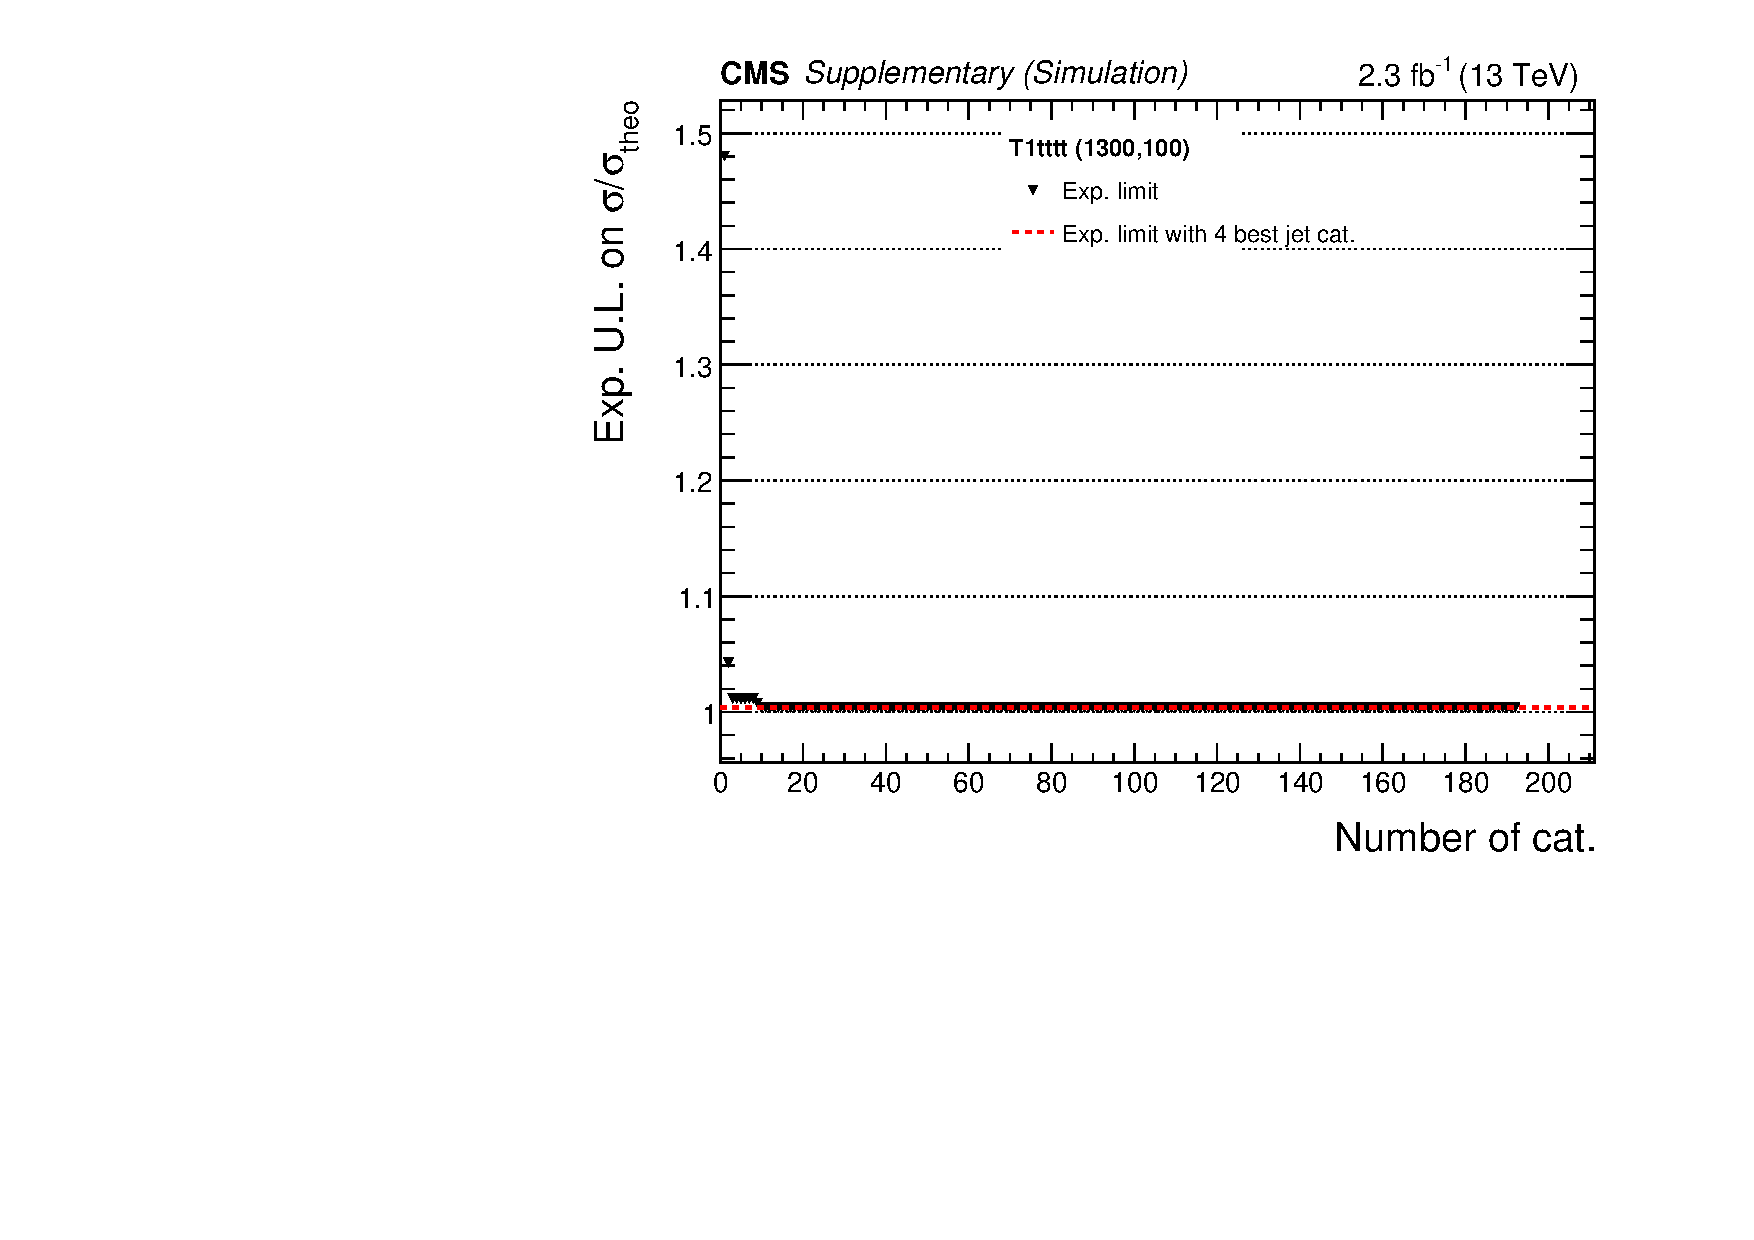
\includegraphics[width=0.49\textwidth]{supplementary/figures/expVsCat_SMS-T1tttt_mGluino-1300_mLSP-100_25ns} \, 
    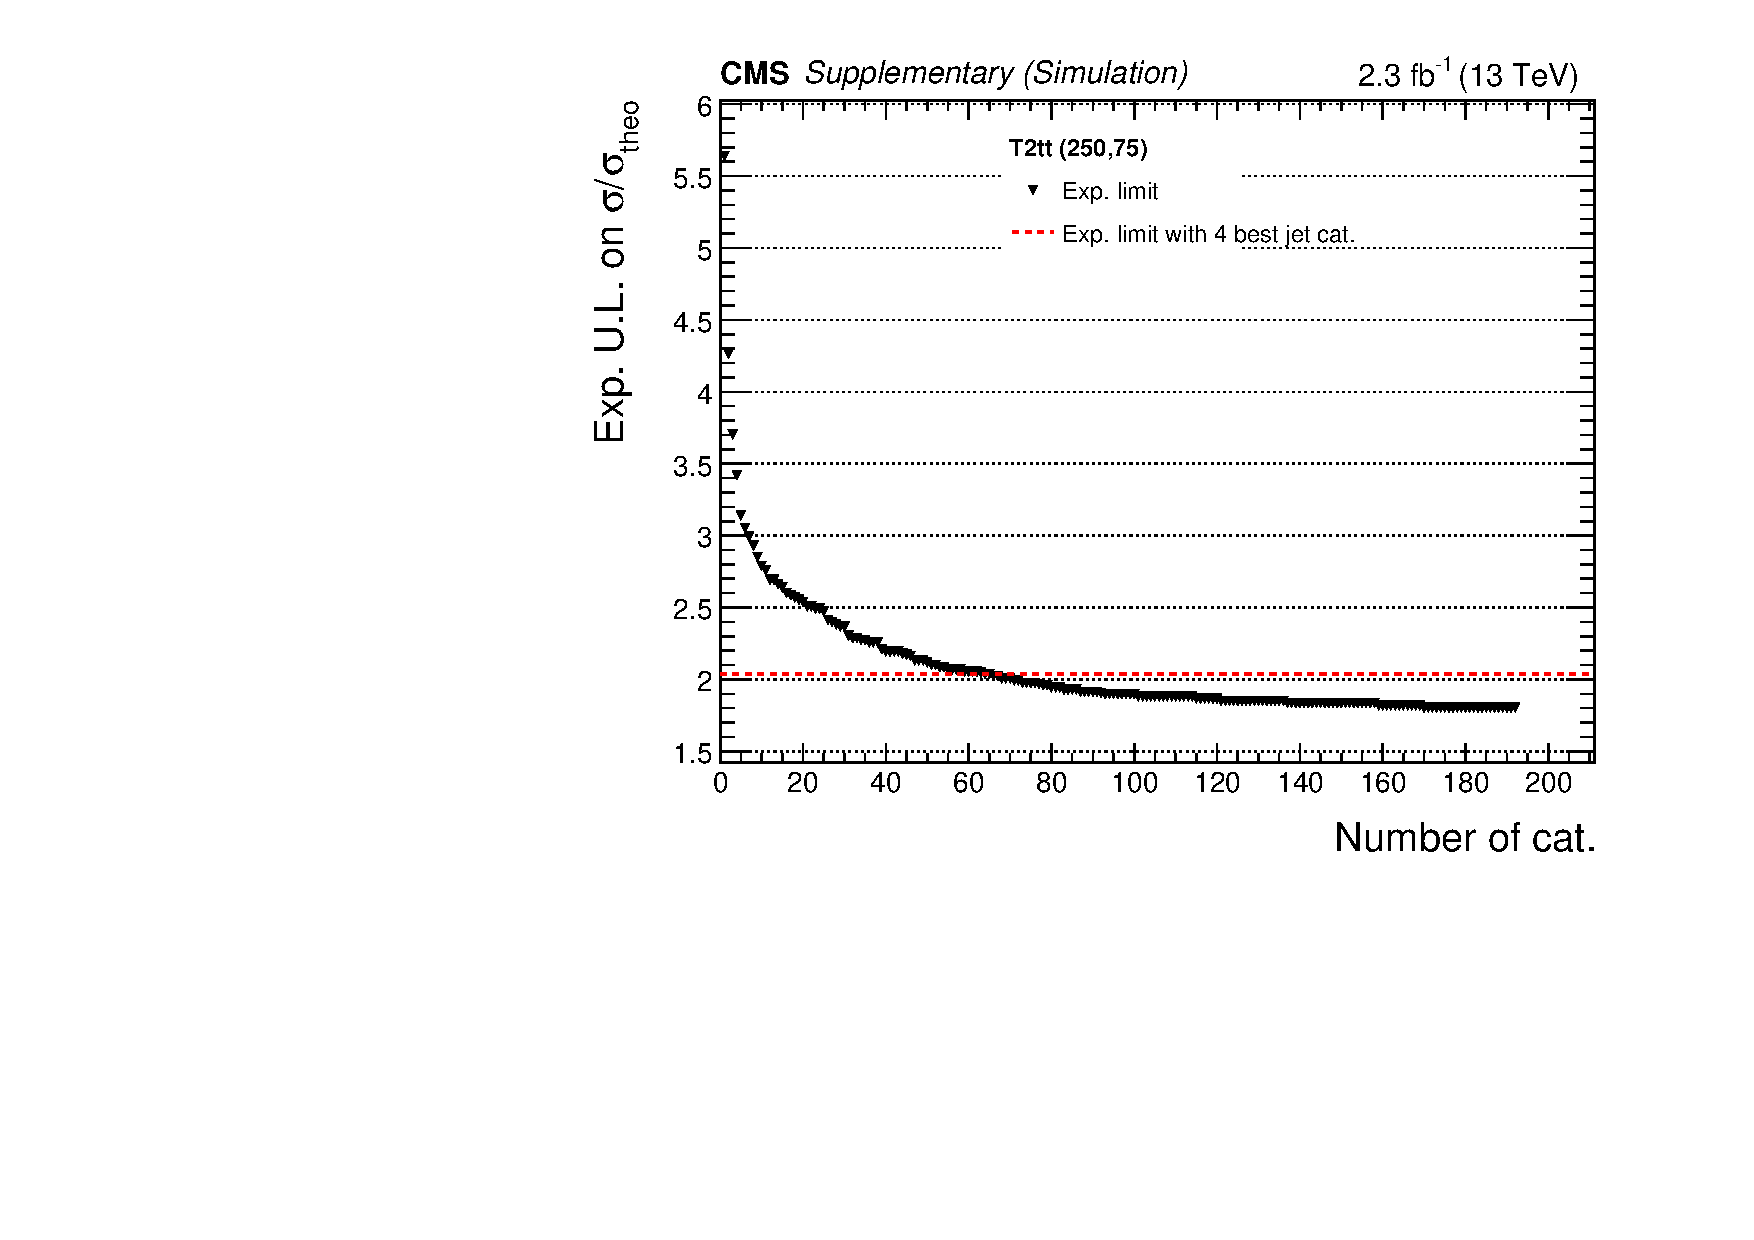
\includegraphics[width=0.49\textwidth]{supplementary/figures/expVsCat_SMS-T2tt_mStop-250_mLSP-75_25ns} \,     
  \end{center}
  \caption{
  The expected upper limit (black points) on the signal strength $\sigma/\sigma_{\mathrm{theo}}$ as a function of the number of 
  (\nj,\nb,\scalht) categories included in the fit, where the categories are ranked according to the expected exclusion, 
  for one T1tttt (T2tt) benchmark point on the left (right) plot. 
  The red dashed line is the expected upper limit using the most excluding 4 jet categories (with all the \nb,\scalht bins within each jet category), 
  as it used for the final limit calculation in this analysis. 
  For the purpose of this test the MC statistical uncertainty in each bin has not been considered. 
  It should be kept in mind that in the analysis jet categories are always considered with all their \nb,\scalht bins 
  combined, in order to preserve the correlation of the systematic uncertainties. 
  Therefore the study depicted by the black points has to be regarded only as an approximate indication 
  of the number of categories contributing to the exclusion, as some of the correlations may be neglected.
  \label{fig:sensitivityVsCat}}
\end{figure*}




\clearpage
\begin{figure*}[t]
  \begin{center}
    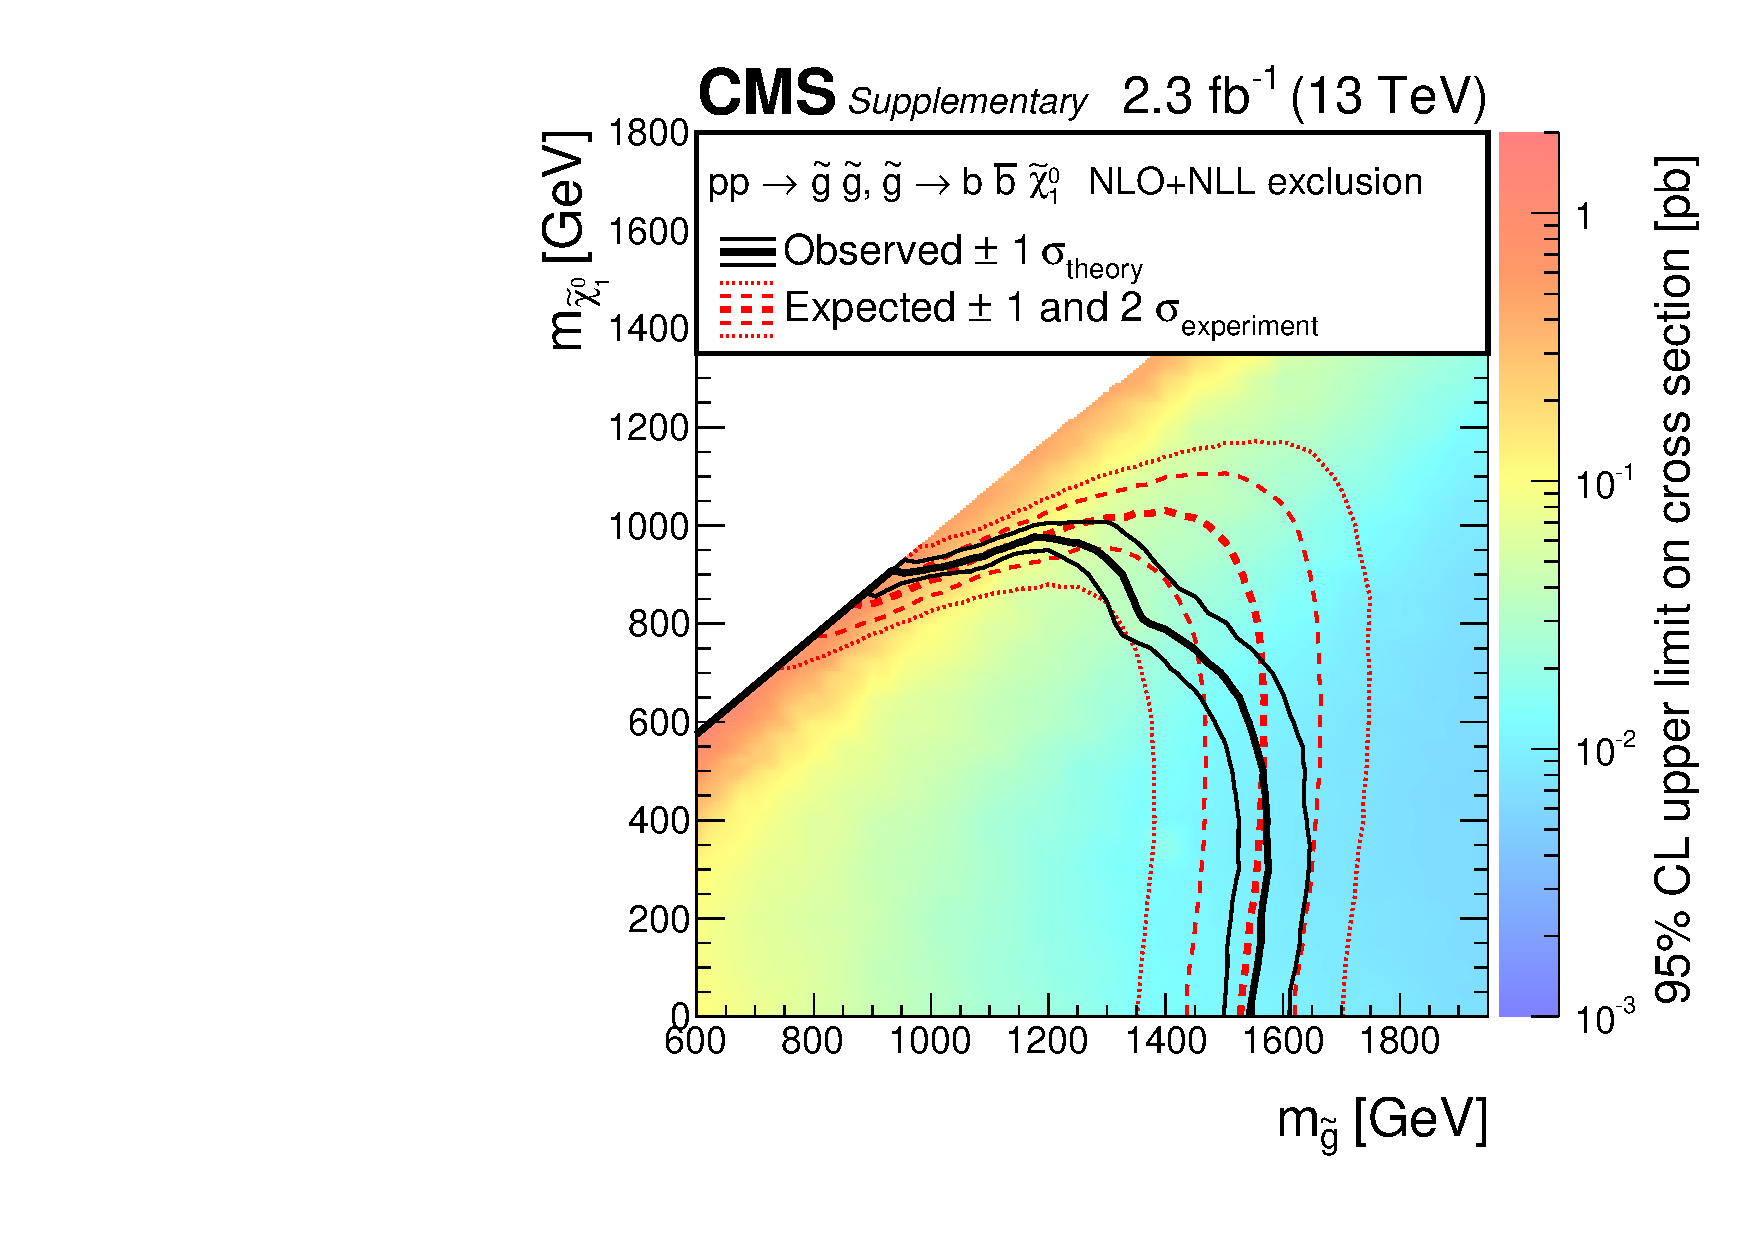
\includegraphics[width=0.49\textwidth]{supplementary/figures/RA1T1bbbbXSEC} \, 
    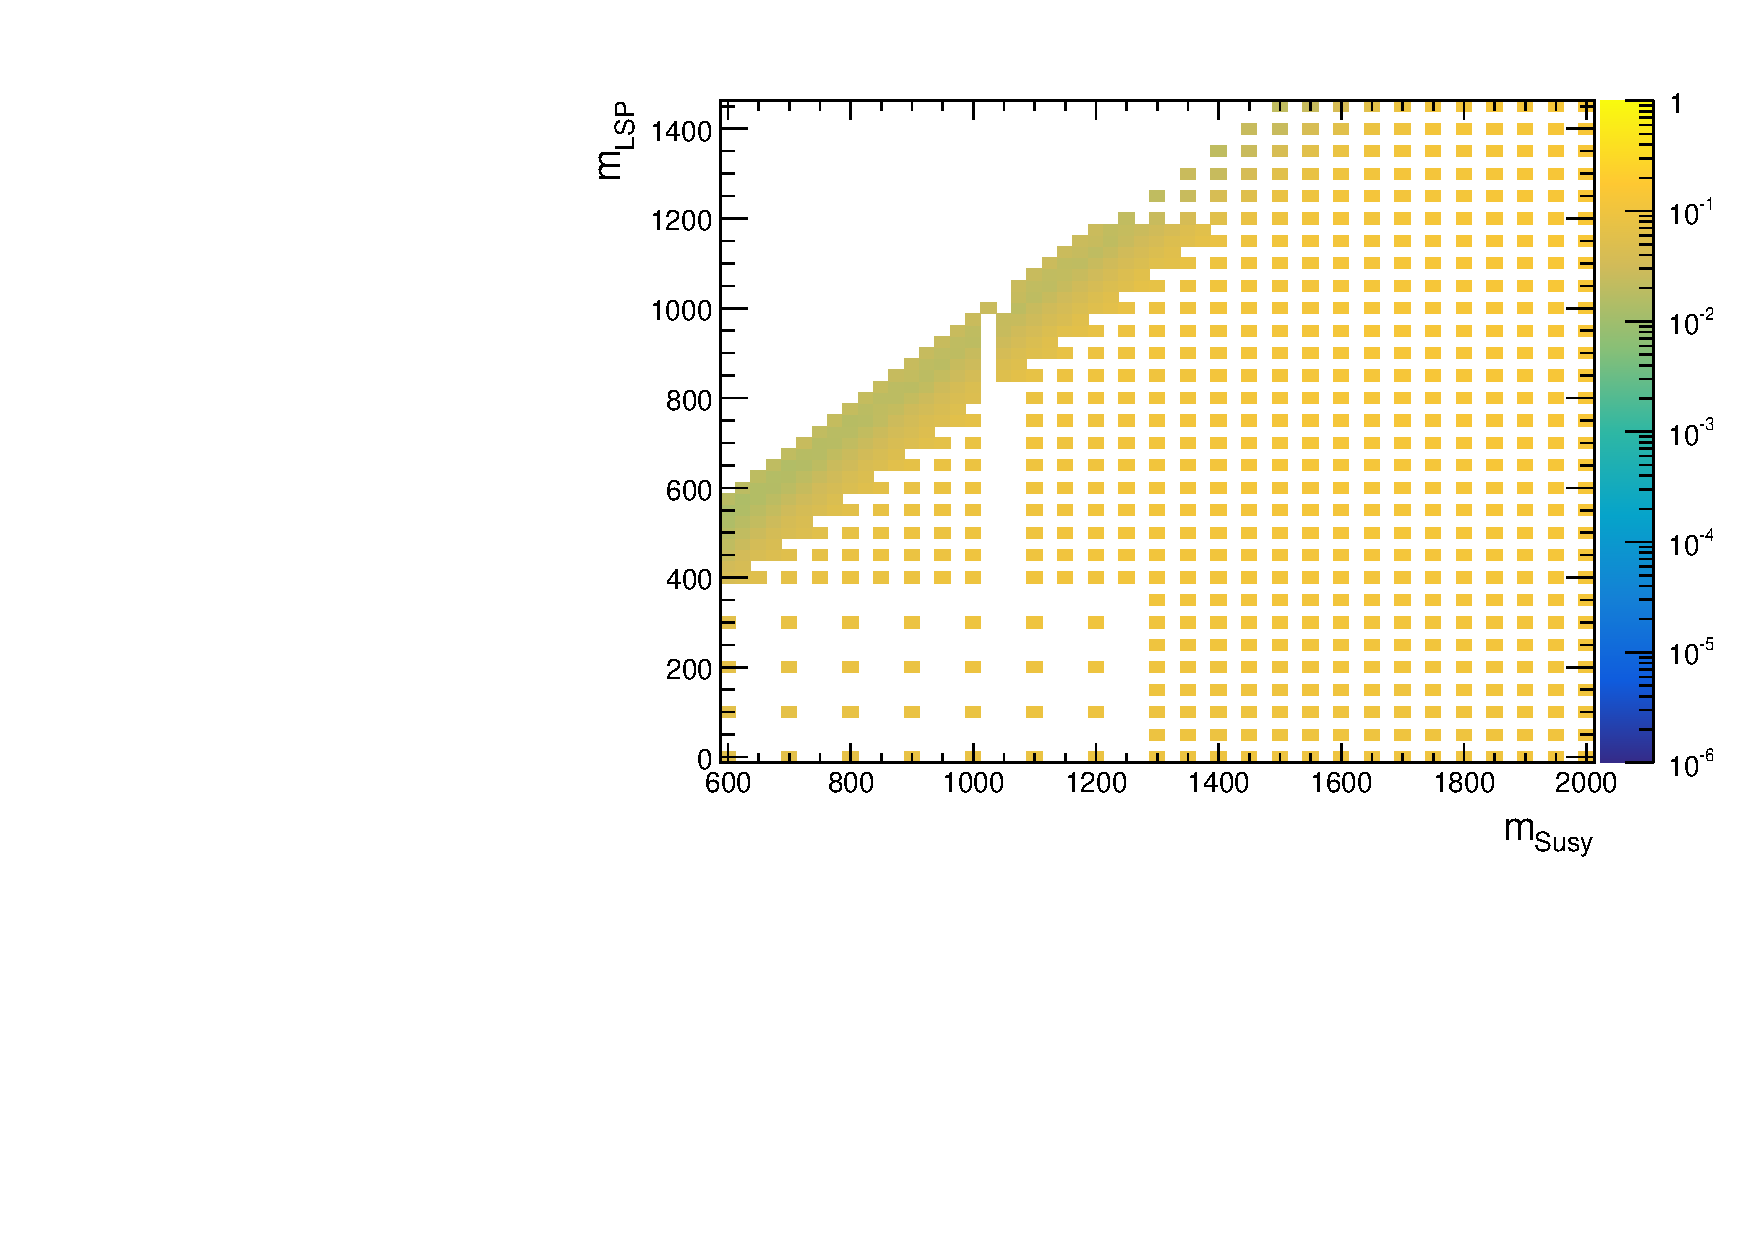
\includegraphics[width=0.49\textwidth]{supplementary/figures/T1bbbb_merging_4_cats} \,     
  \end{center}
  \caption{Left: (coloured histogram) upper limit on the cross section in the $(m_{\mathrm{Gluino}},m_{\mathrm{LSP}})$ plane for the T1bbbb model. 
  The black (red) solid line is the observed (expected) exclusion. The red dashed lines are the $\pm1\sigma$ expected exclusion due to experimental uncertainties. 
  The $\pm1\sigma$ observed exclusion due to theoretical uncertainties on the signal cross section are shown as thin black lines. 
  Right: signal efficiency for the search regions included in the limit calculation as a function $(m_{\mathrm{Gluino}},m_{\mathrm{LSP}})$ plane for the T1bbbb model. 
  \label{fig:T1bbbb_excl}}
\end{figure*}

\begin{figure*}[t]
  \begin{center}
    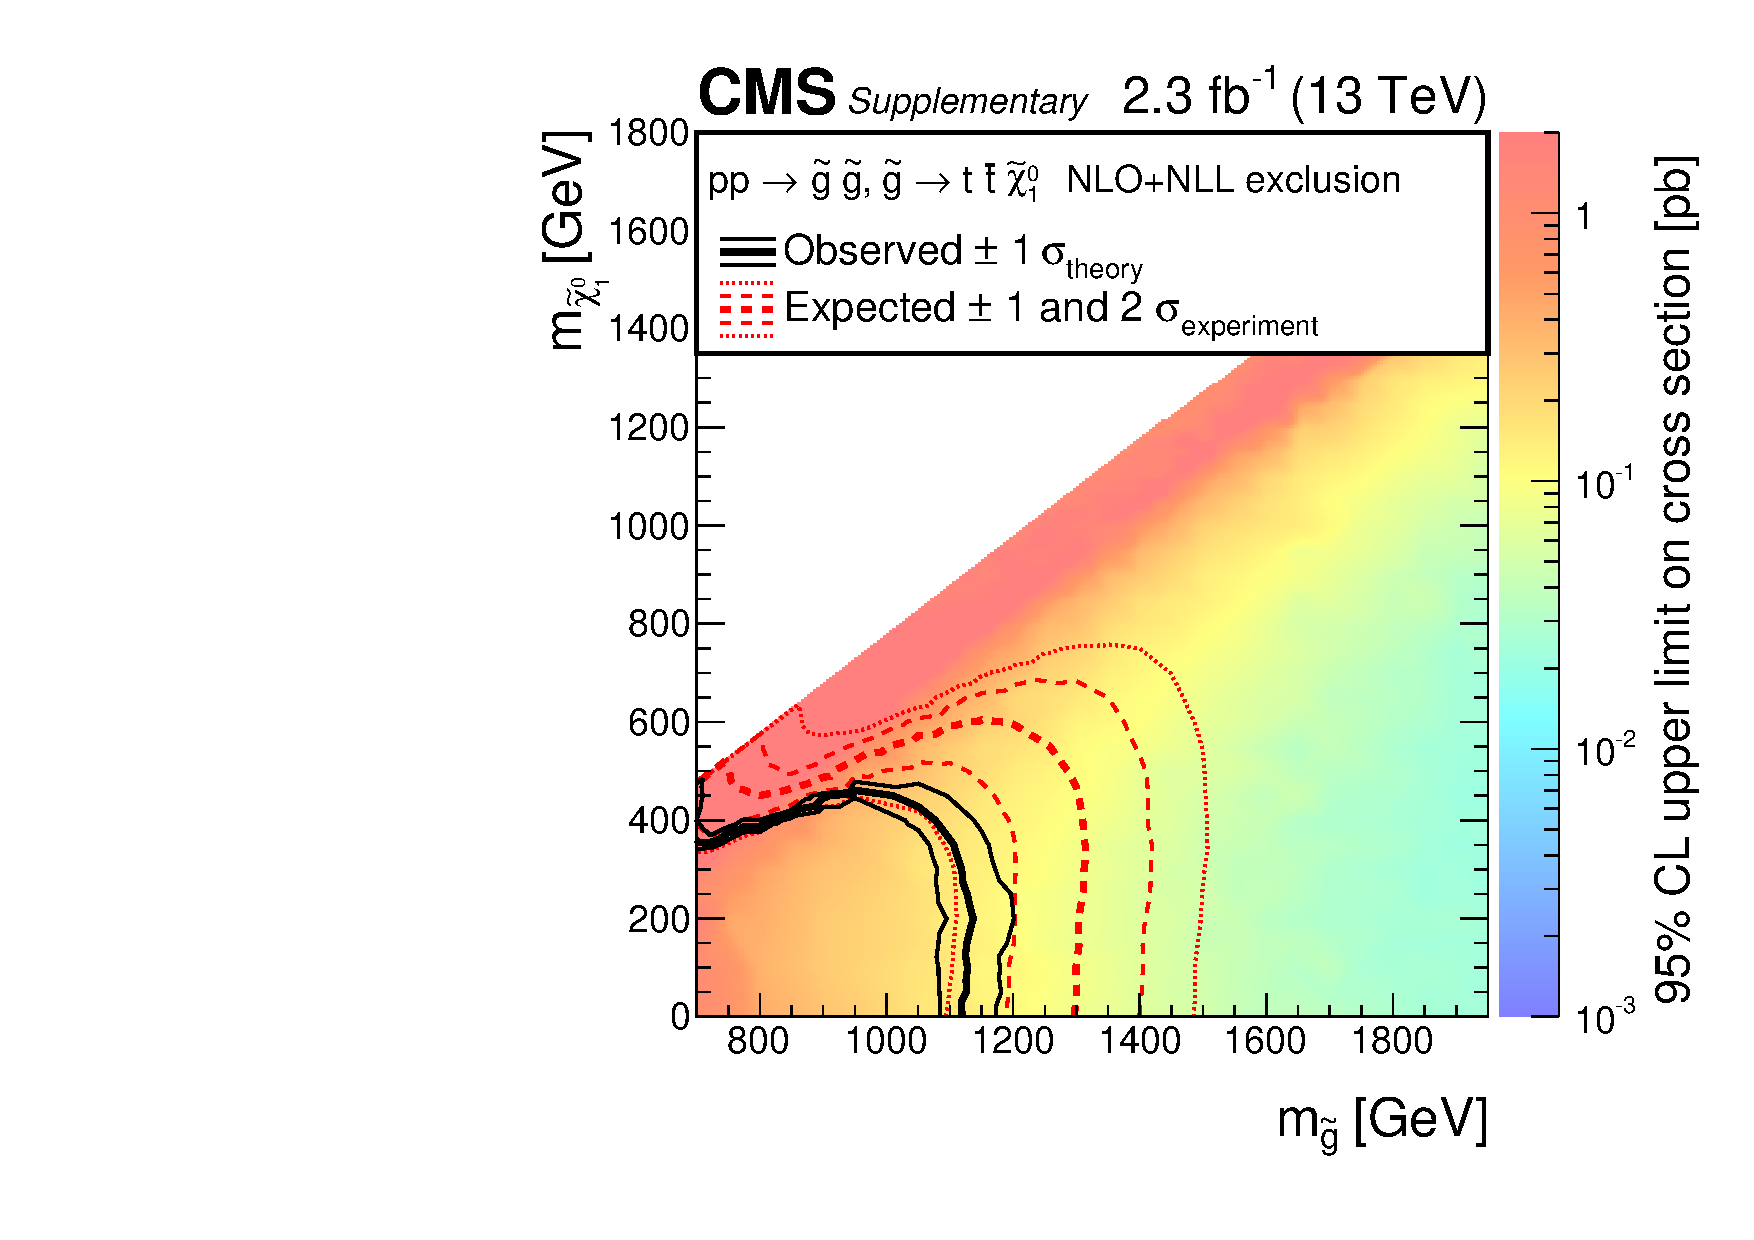
\includegraphics[width=0.49\textwidth]{supplementary/figures/RA1T1ttttXSEC} \, 
    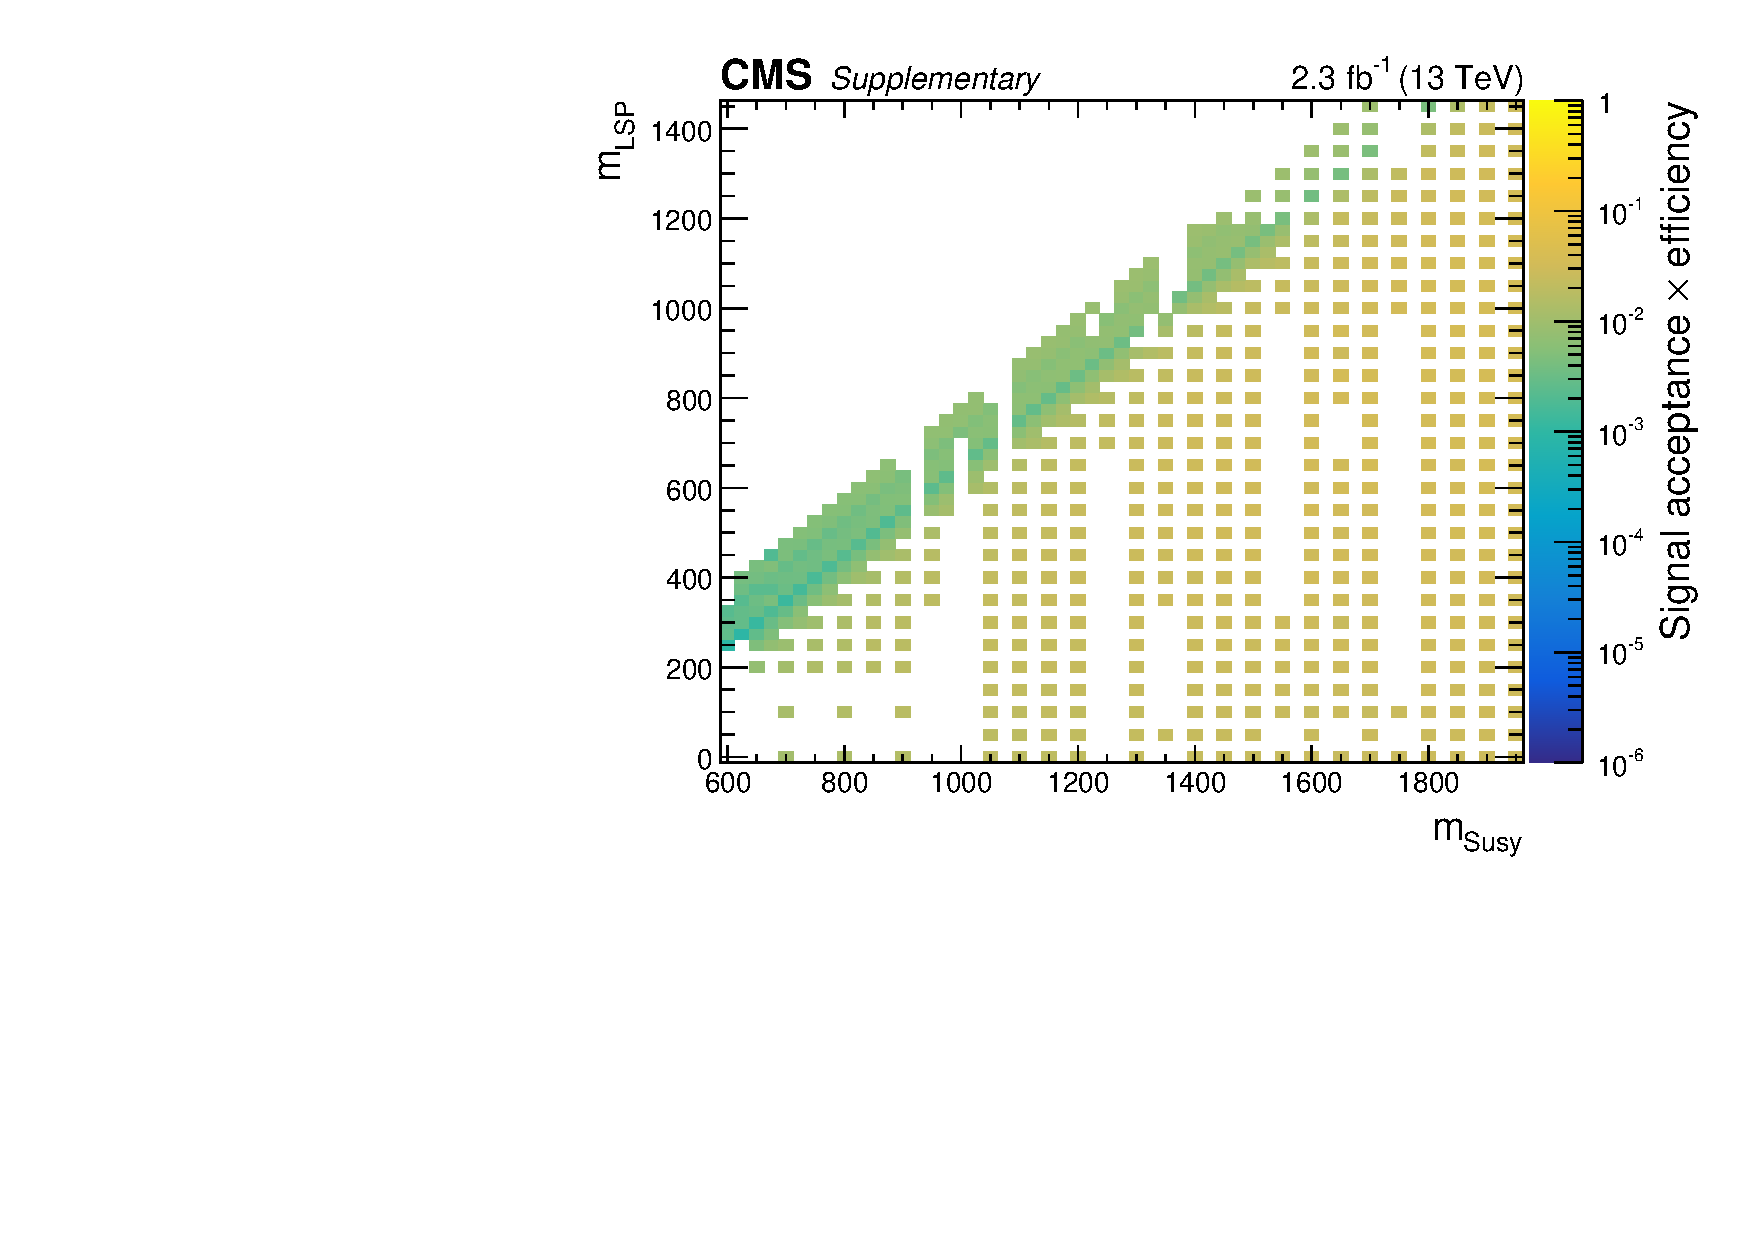
\includegraphics[width=0.49\textwidth]{supplementary/figures/T1tttt_merging_4_cats} \,     
  \end{center}
  \caption{Left: (coloured histogram) upper limit on the cross section in the $(m_{\mathrm{Gluino}},m_{\mathrm{LSP}})$ plane for the T1tttt model. 
  The black (red) solid line is the observed (expected) exclusion. The red dashed lines are the $\pm1\sigma$ expected exclusion due to experimental uncertainties. 
  The $\pm1\sigma$ observed exclusion due to theoretical uncertainties on the signal cross section are shown as thin black lines. 
  Right: signal efficiency for the search regions included in the limit calculation as a function $(m_{\mathrm{Gluino}},m_{\mathrm{LSP}})$ plane for the T1tttt model. 
  \label{fig:T1tttt_excl}}
\end{figure*}

\clearpage
\begin{figure*}[t]
  \begin{center}
    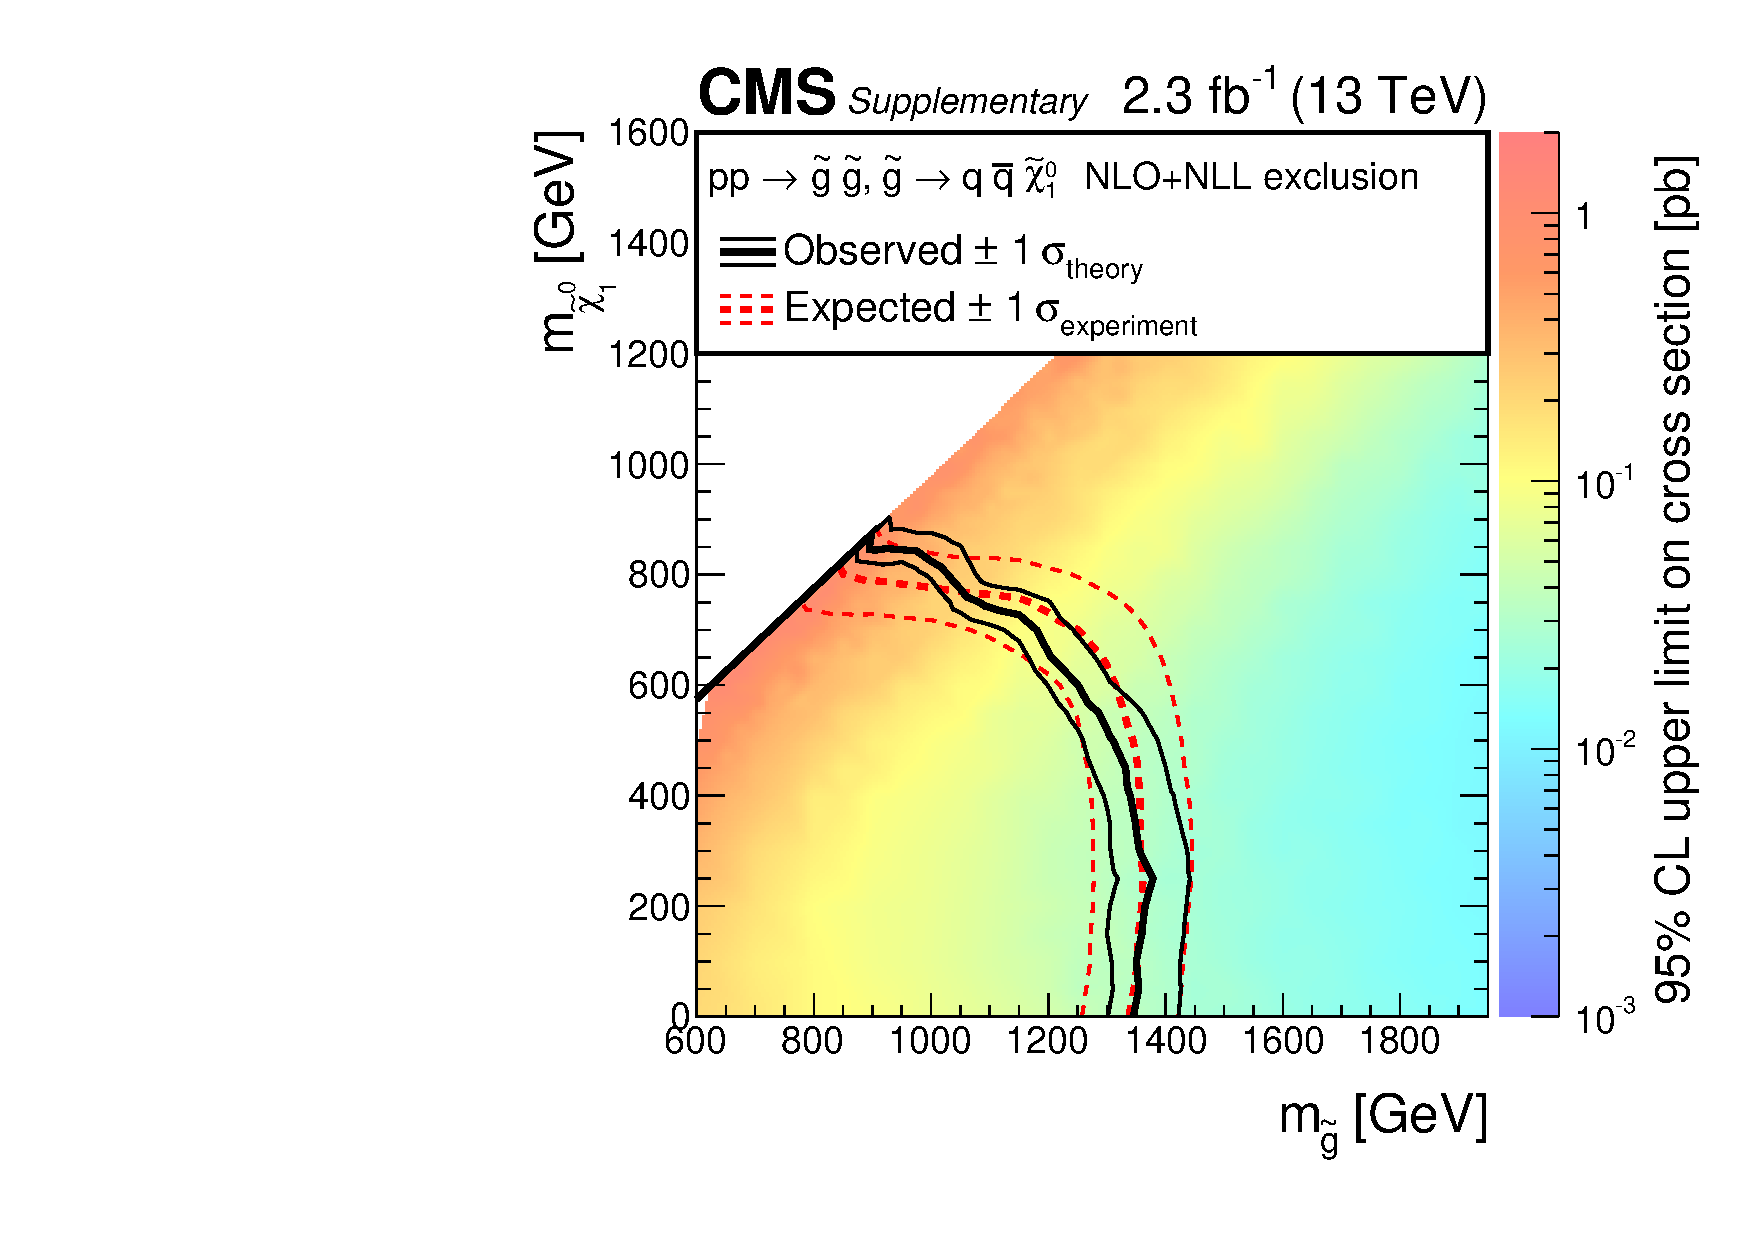
\includegraphics[width=0.49\textwidth]{supplementary/figures/RA1T1qqqqXSEC} \, 
    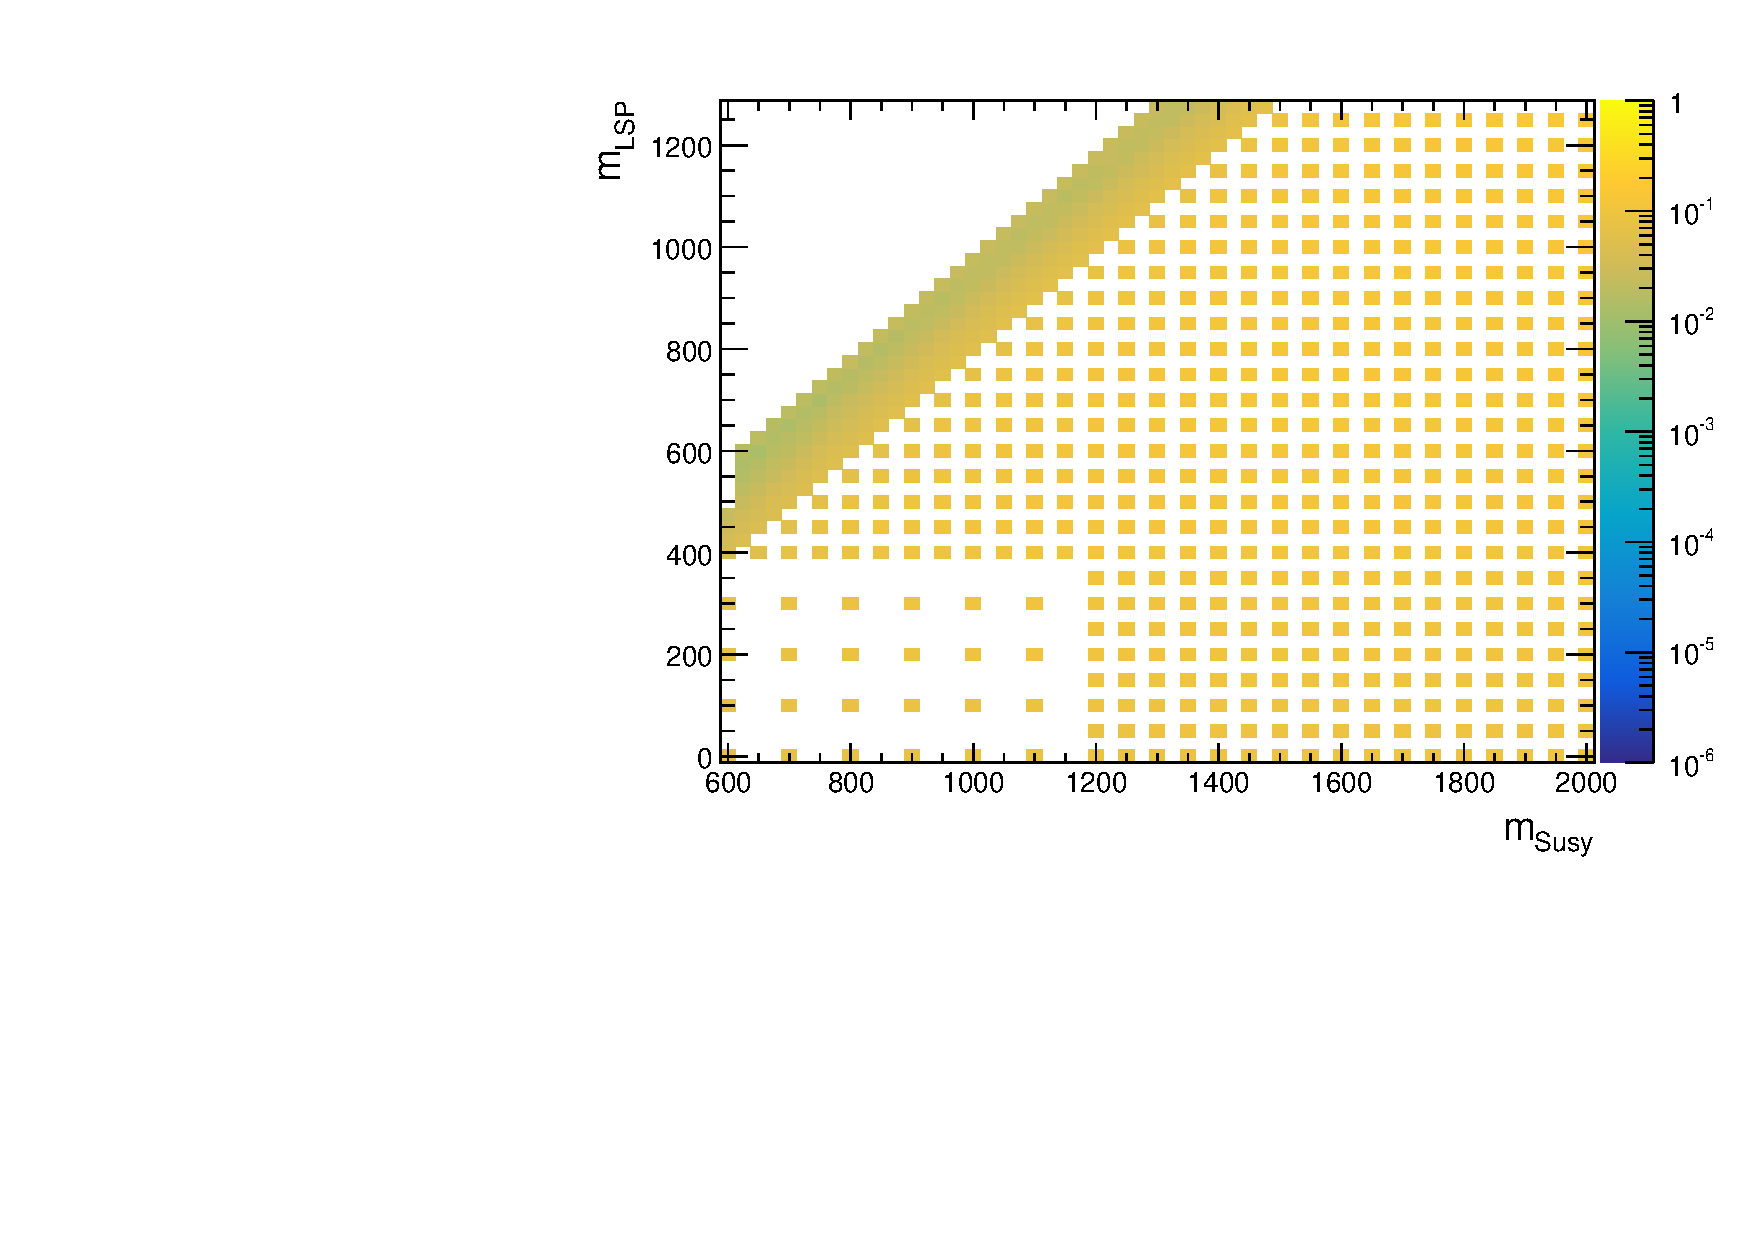
\includegraphics[width=0.49\textwidth]{supplementary/figures/T1qqqq_merging_4_cats} \,     
  \end{center}
  \caption{Left: (coloured histogram) upper limit on the cross section in the $(m_{\mathrm{Gluino}},m_{\mathrm{LSP}})$ plane for the T1qqqq model. 
  The black (red) solid line is the observed (expected) exclusion. The red dashed lines are the $\pm1\sigma$ expected exclusion due to experimental uncertainties. 
  The $\pm1\sigma$ observed exclusion due to theoretical uncertainties on the signal cross section are shown as thin black lines. 
  Right: signal efficiency for the search regions included in the limit calculation as a function $(m_{\mathrm{Gluino}},m_{\mathrm{LSP}})$ plane for the T1qqqq model. 
  \label{fig:T1qqqq_excl}}
\end{figure*}

\begin{figure*}[t]
  \begin{center}
    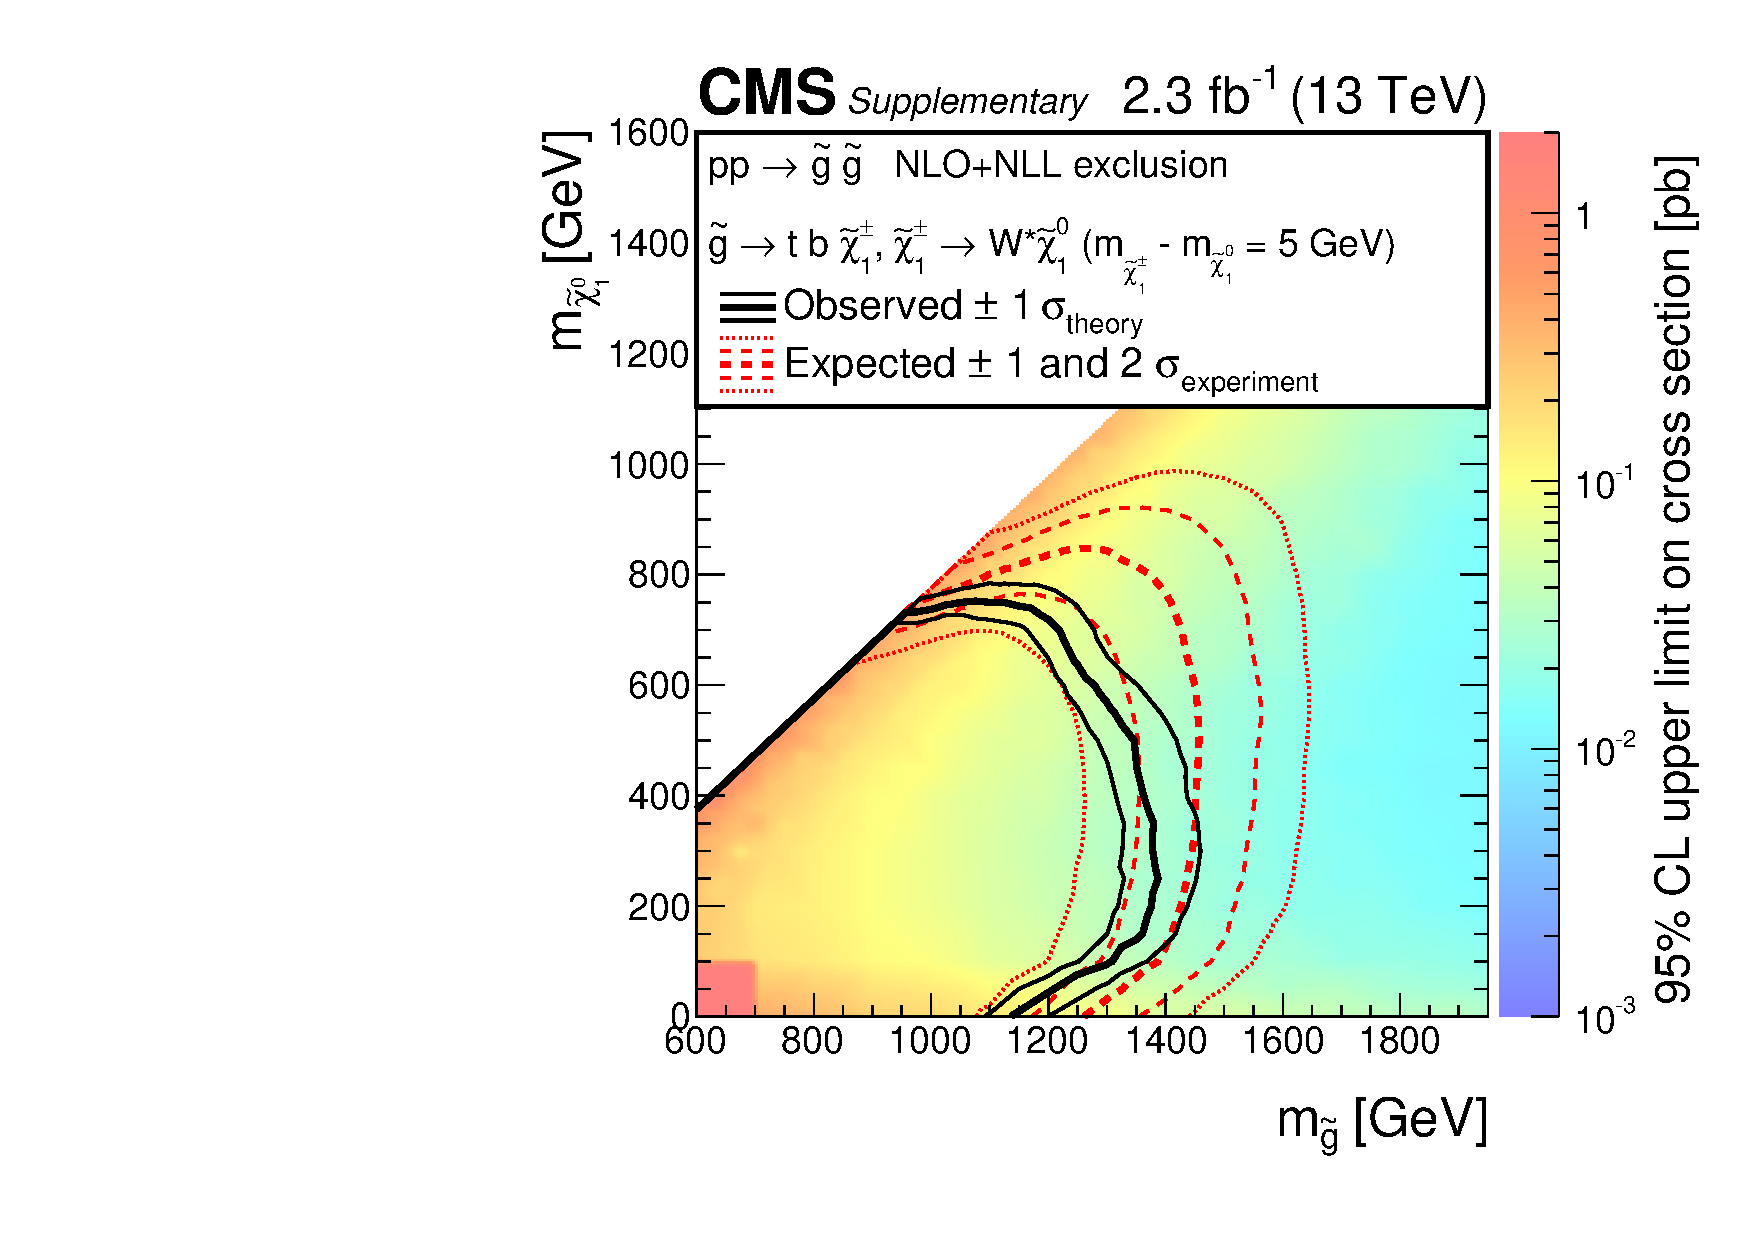
\includegraphics[width=0.49\textwidth]{supplementary/figures/RA1T1ttbbXSEC} \, 
    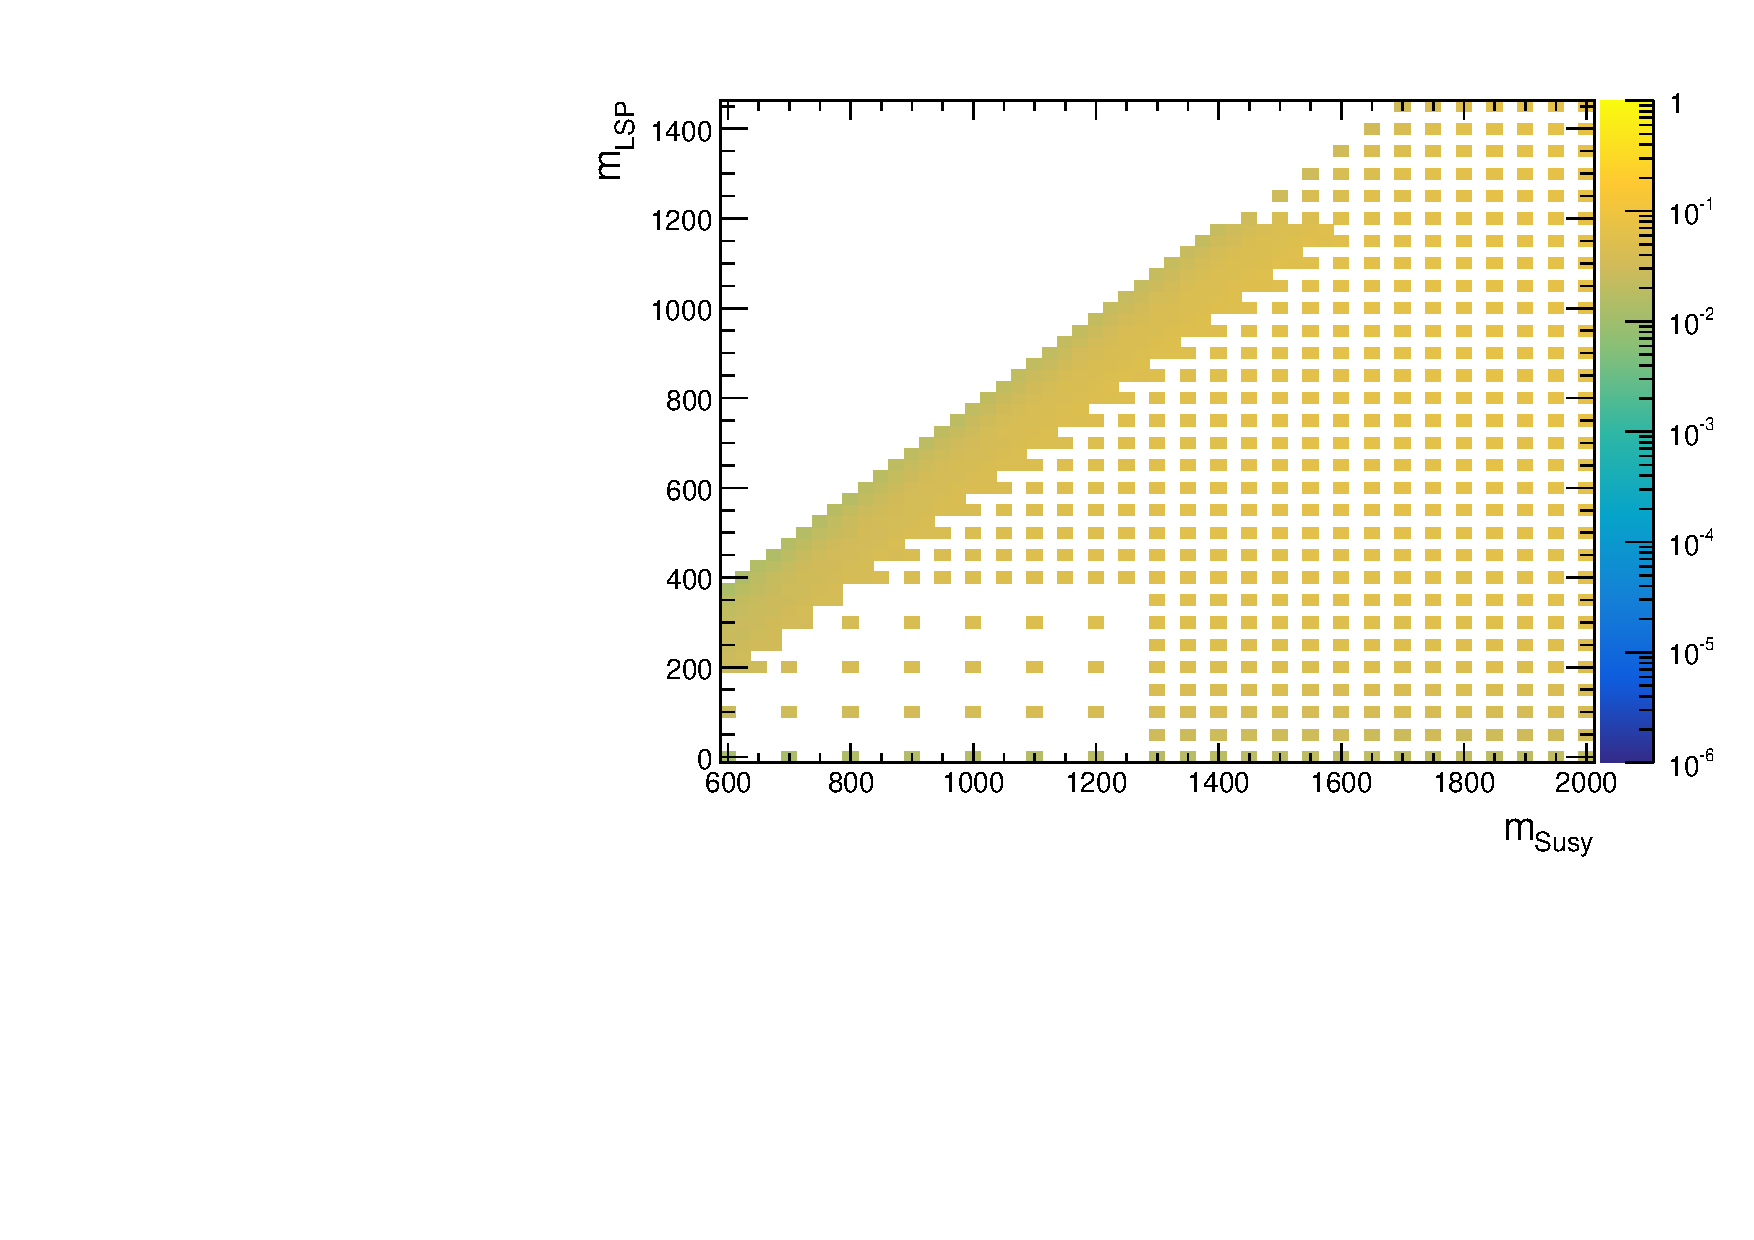
\includegraphics[width=0.49\textwidth]{supplementary/figures/T1ttbb_merging_4_cats} \,     
  \end{center}
  \caption{Left: (coloured histogram) upper limit on the cross section in the $(m_{\mathrm{Gluino}},m_{\mathrm{LSP}})$ plane for the T1ttbb model. 
  The black (red) solid line is the observed (expected) exclusion. The red dashed lines are the $\pm1\sigma$ expected exclusion due to experimental uncertainties. 
  The $\pm1\sigma$ observed exclusion due to theoretical uncertainties on the signal cross section are shown as thin black lines. 
  Right: signal efficiency for the search regions included in the limit calculation as a function $(m_{\mathrm{Gluino}},m_{\mathrm{LSP}})$ plane for the T1ttbb model. 
  \label{fig:T1ttbb_excl}}
\end{figure*}


\clearpage
\begin{figure*}[t]
  \begin{center}
    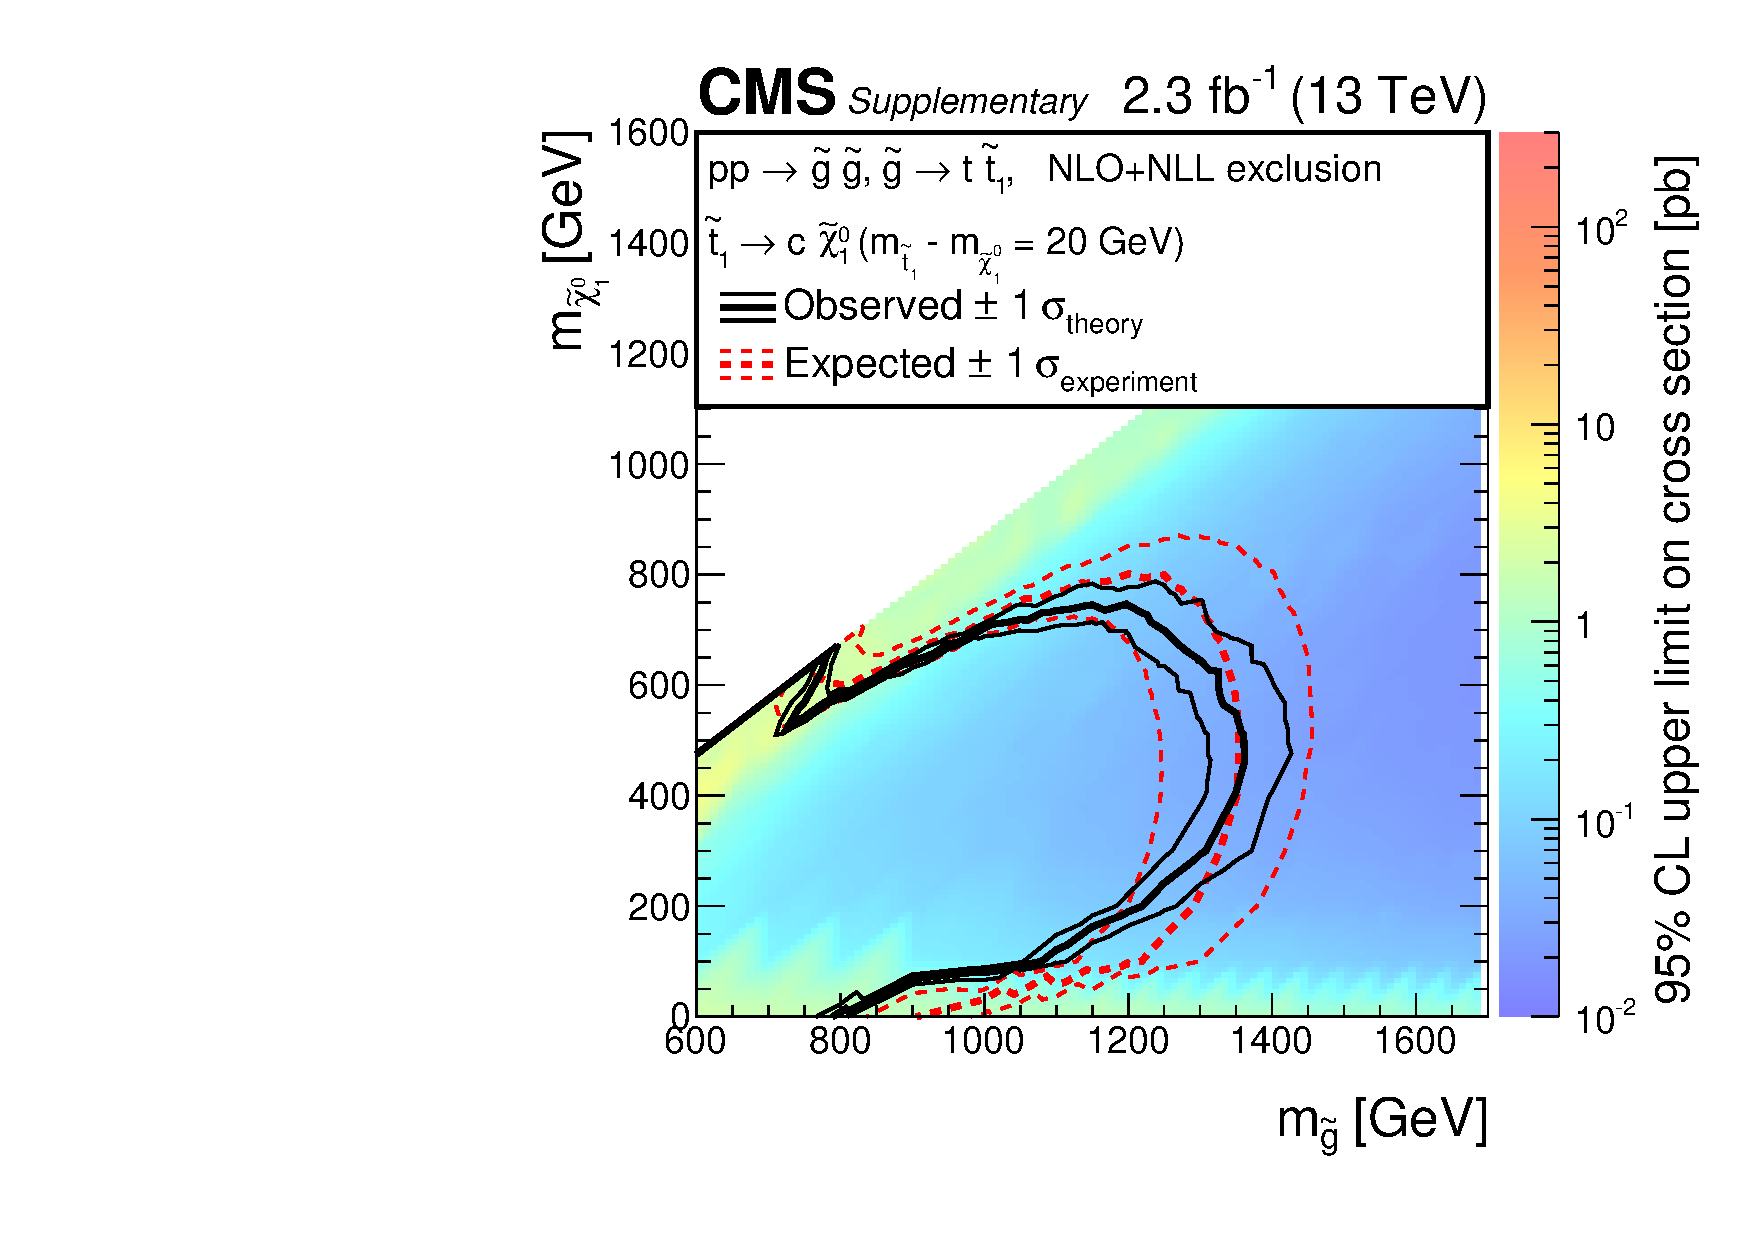
\includegraphics[width=0.49\textwidth]{supplementary/figures/RA1T5ttccXSEC} \, 
    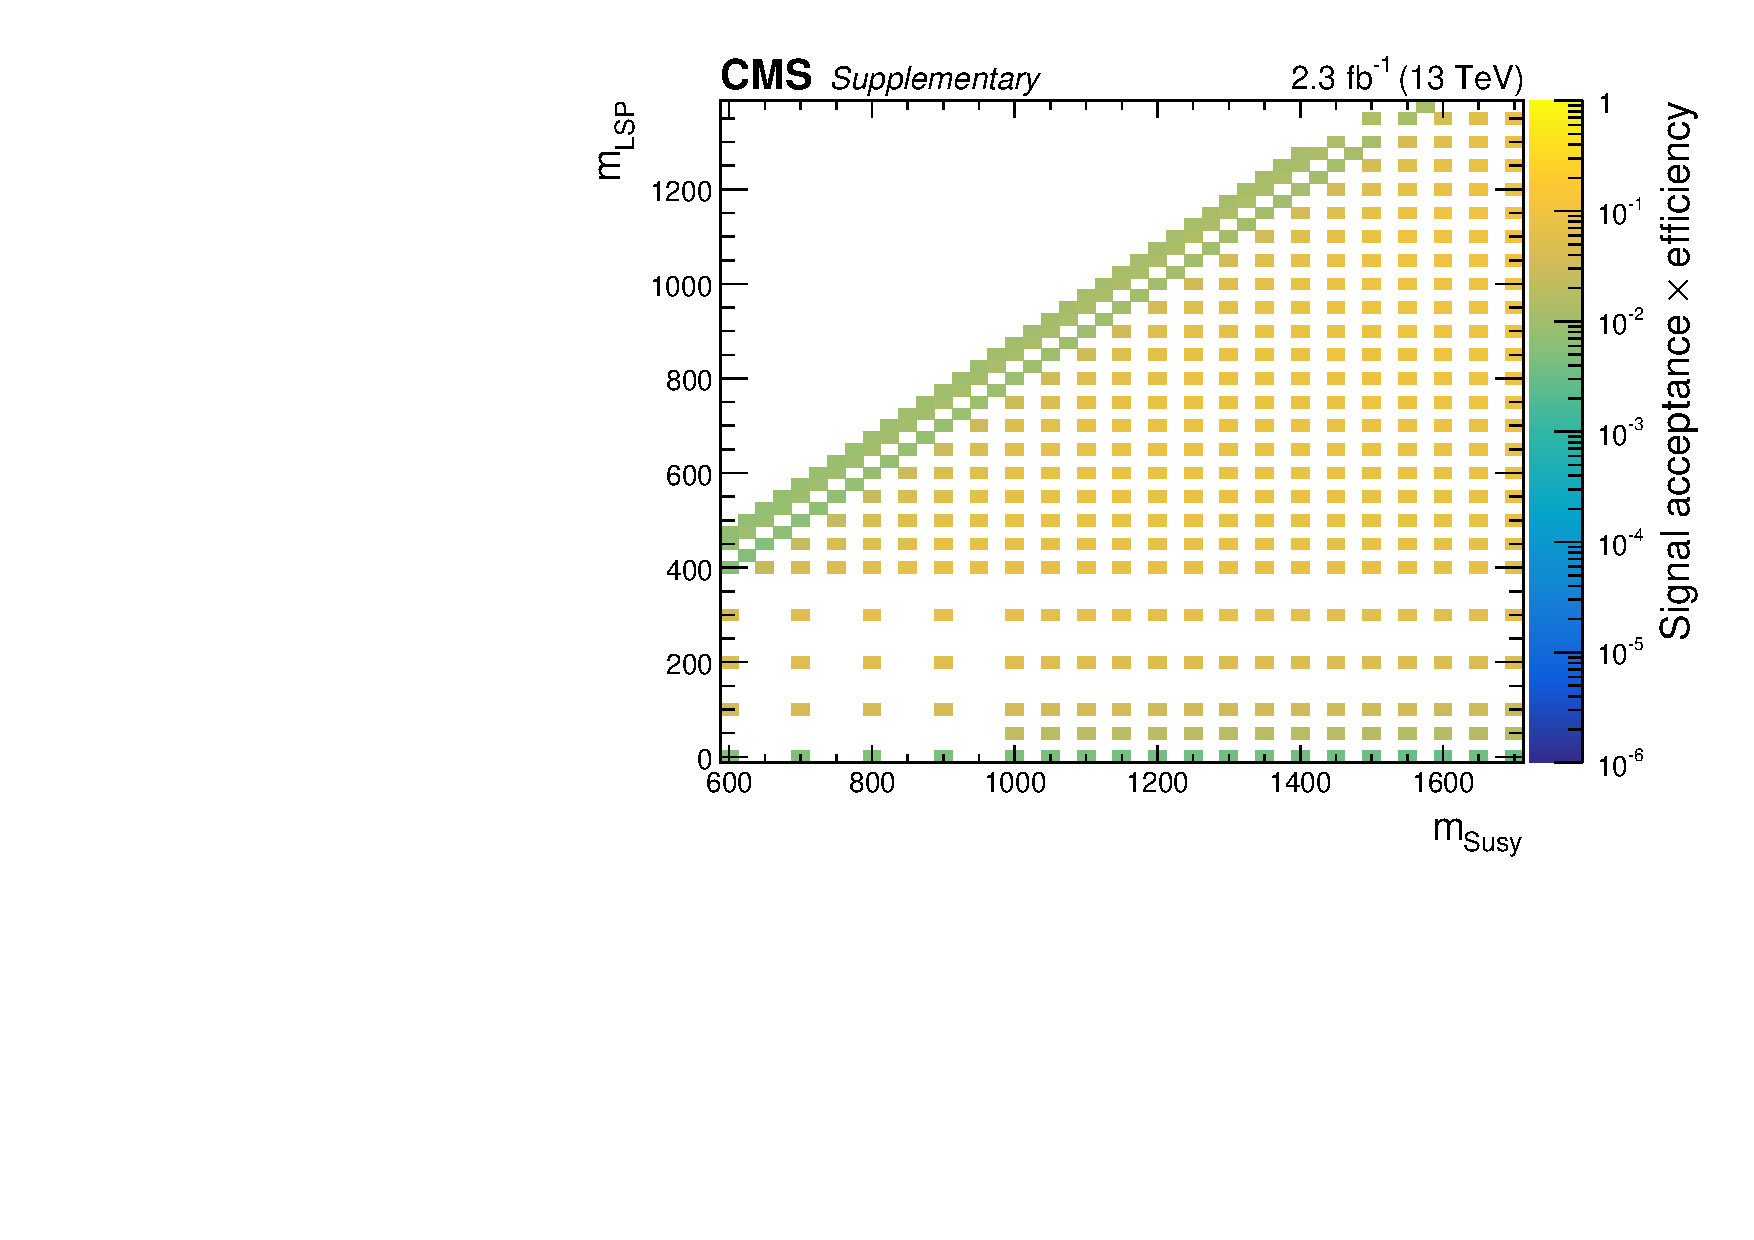
\includegraphics[width=0.49\textwidth]{supplementary/figures/T5ttcc_merging_4_cats} \,     
  \end{center}
  \caption{Left: (coloured histogram) upper limit on the cross section in the $(m_{\mathrm{Gluino}},m_{\mathrm{LSP}})$ plane for the T5ttcc model. 
  The black (red) solid line is the observed (expected) exclusion. The red dashed lines are the $\pm1\sigma$ expected exclusion due to experimental uncertainties. 
  The $\pm1\sigma$ observed exclusion due to theoretical uncertainties on the signal cross section are shown as thin black lines. 
  Right: signal efficiency for the search regions included in the limit calculation as a function $(m_{\mathrm{Gluino}},m_{\mathrm{LSP}})$ plane for the T5ttcc model. 
  \label{fig:T5ttcc_excl}}
\end{figure*}

\begin{figure*}[t]
  \begin{center}
    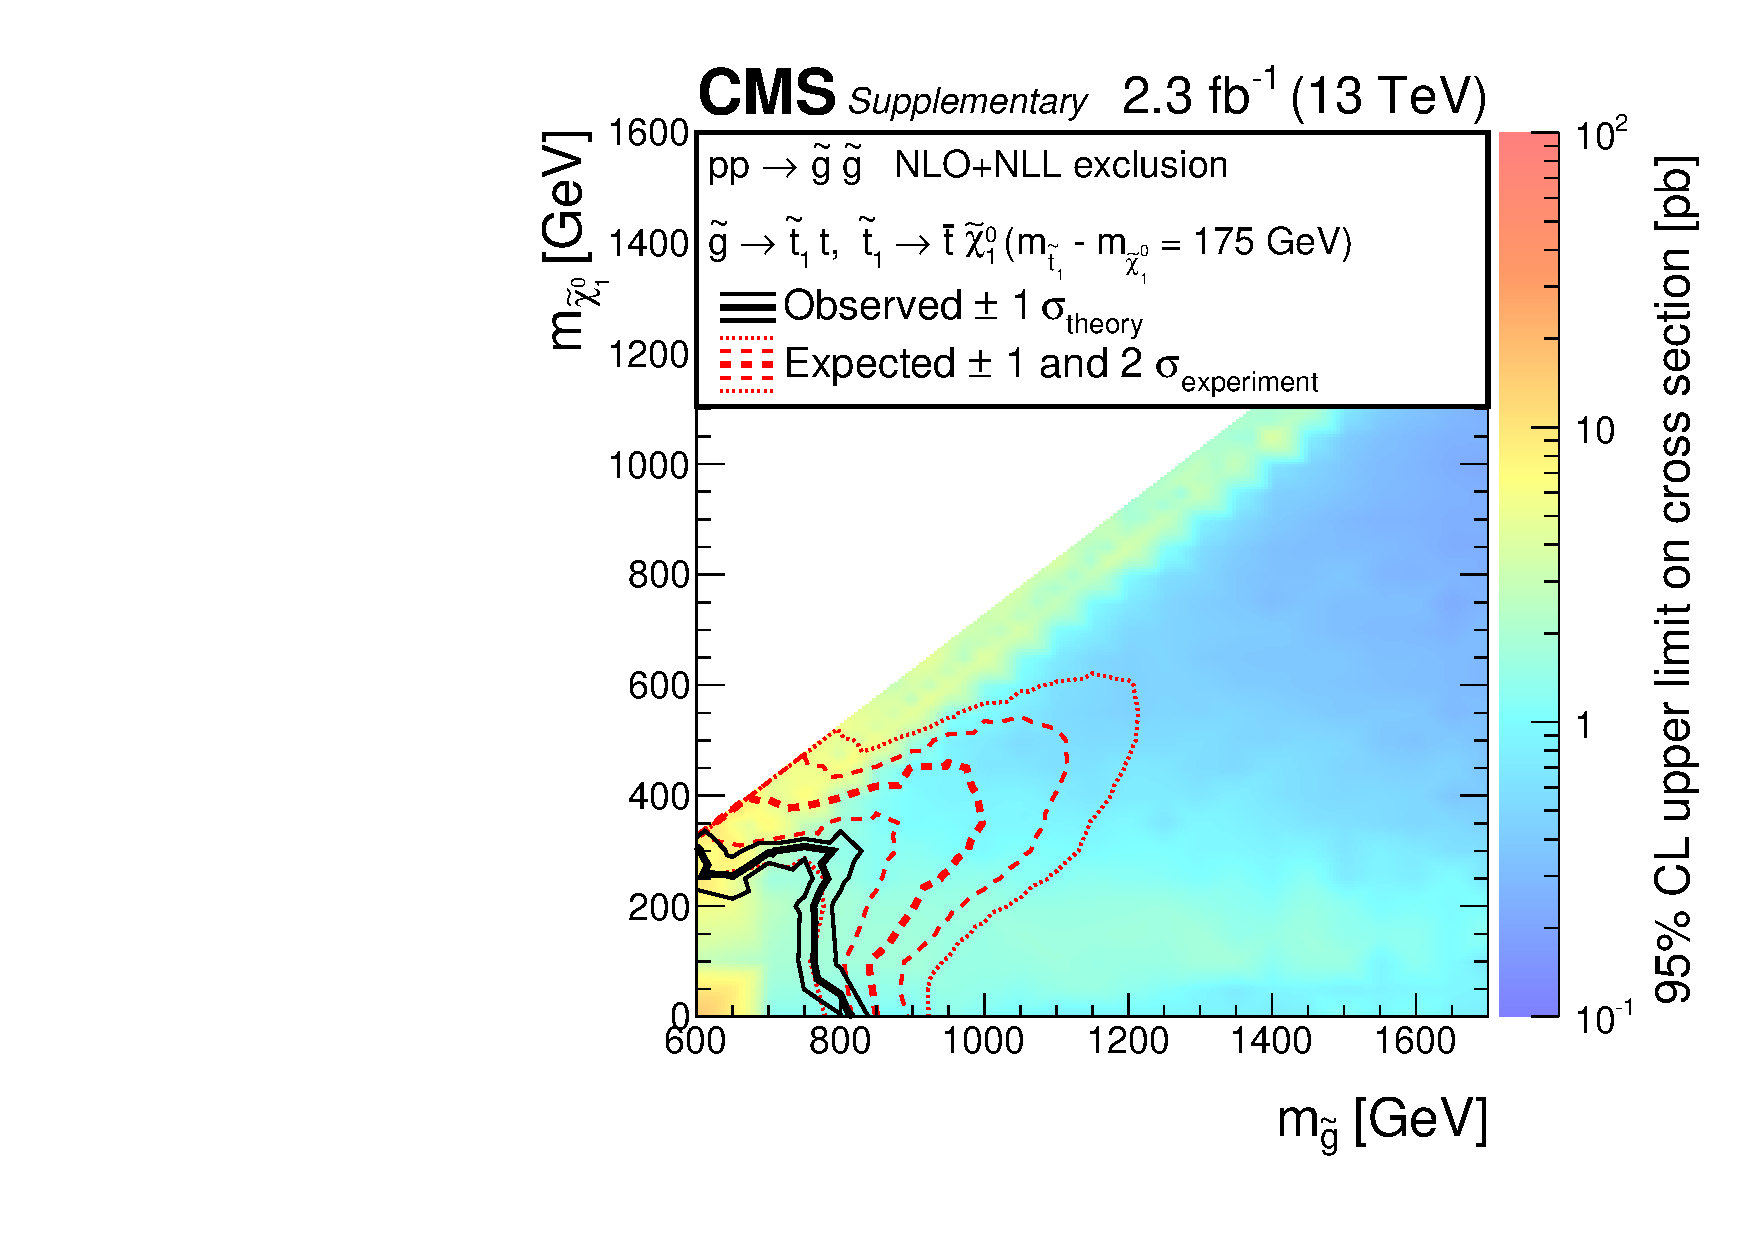
\includegraphics[width=0.49\textwidth]{supplementary/figures/RA1T5ttttDM175XSEC} \, 
    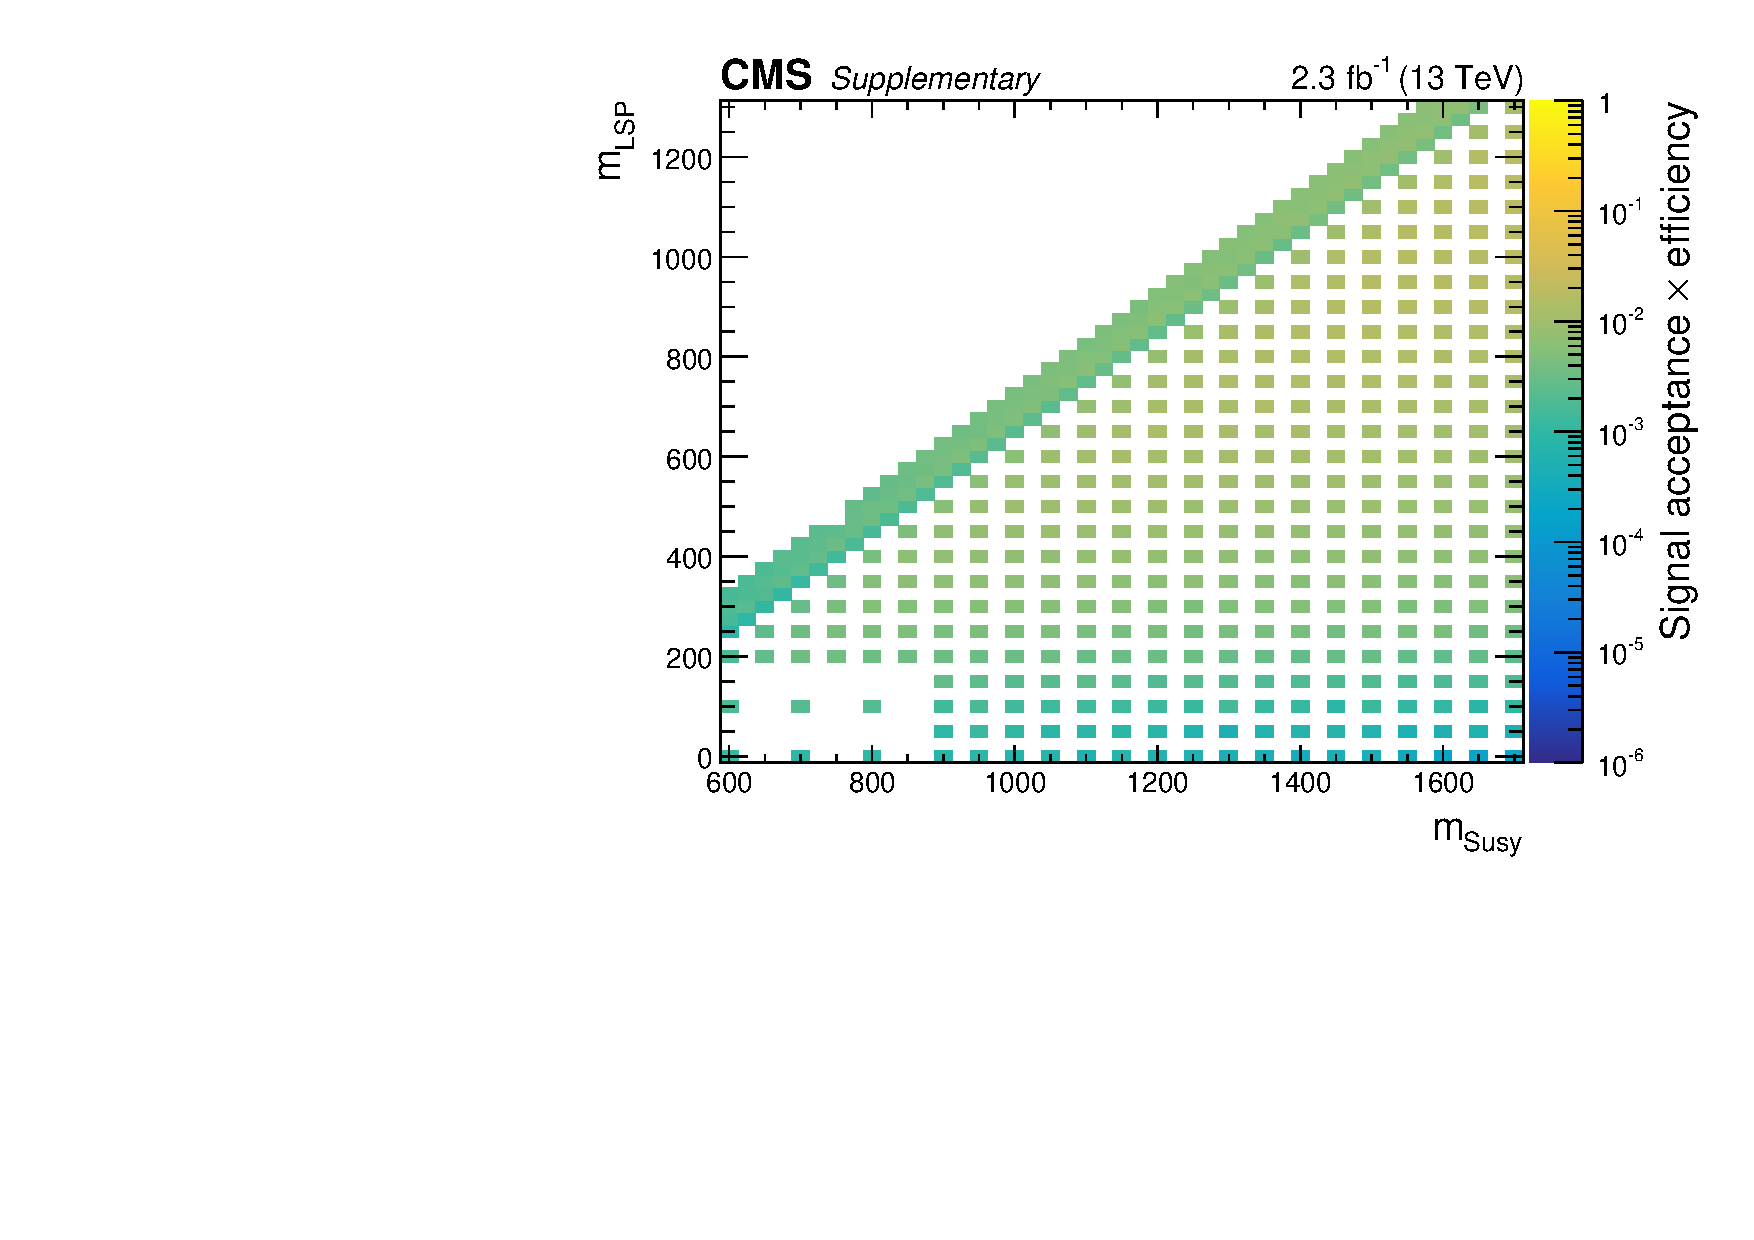
\includegraphics[width=0.49\textwidth]{supplementary/figures/T5ttttDM175_merging_4_cats} \,     
  \end{center}
  \caption{Left: (coloured histogram) upper limit on the cross section in the $(m_{\mathrm{Gluino}},m_{\mathrm{LSP}})$ plane for the T5ttttDM175 model. 
  The black (red) solid line is the observed (expected) exclusion. The red dashed lines are the $\pm1\sigma$ expected exclusion due to experimental uncertainties. 
  The $\pm1\sigma$ observed exclusion due to theoretical uncertainties on the signal cross section are shown as thin black lines. 
  Right: signal efficiency for the search regions included in the limit calculation as a function $(m_{\mathrm{Gluino}},m_{\mathrm{LSP}})$ plane for the T5ttttDM175 model. 
  \label{fig:T5ttttDM175_excl}}
\end{figure*}


\clearpage
\begin{figure*}[t]
  \begin{center}
    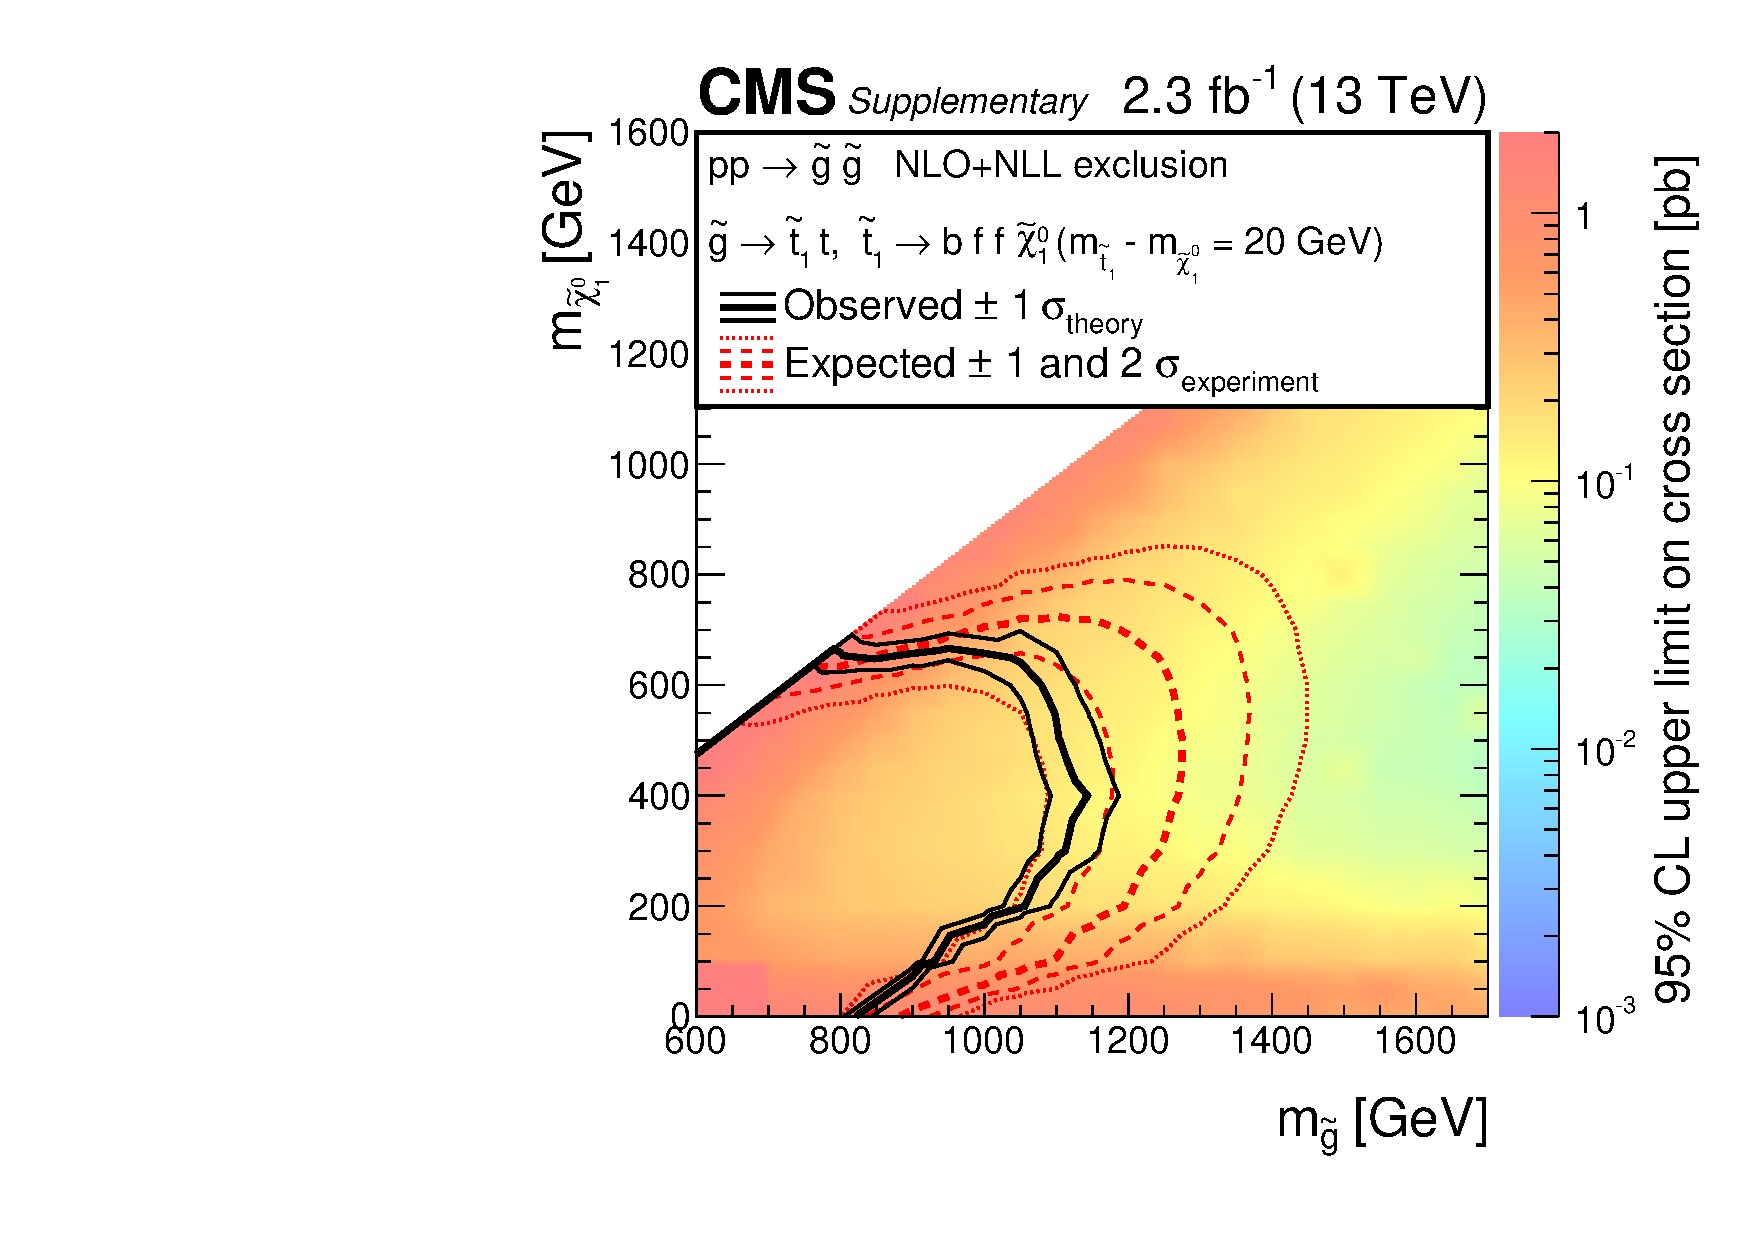
\includegraphics[width=0.49\textwidth]{supplementary/figures/RA1T5tttt-degenXSEC} \, 
    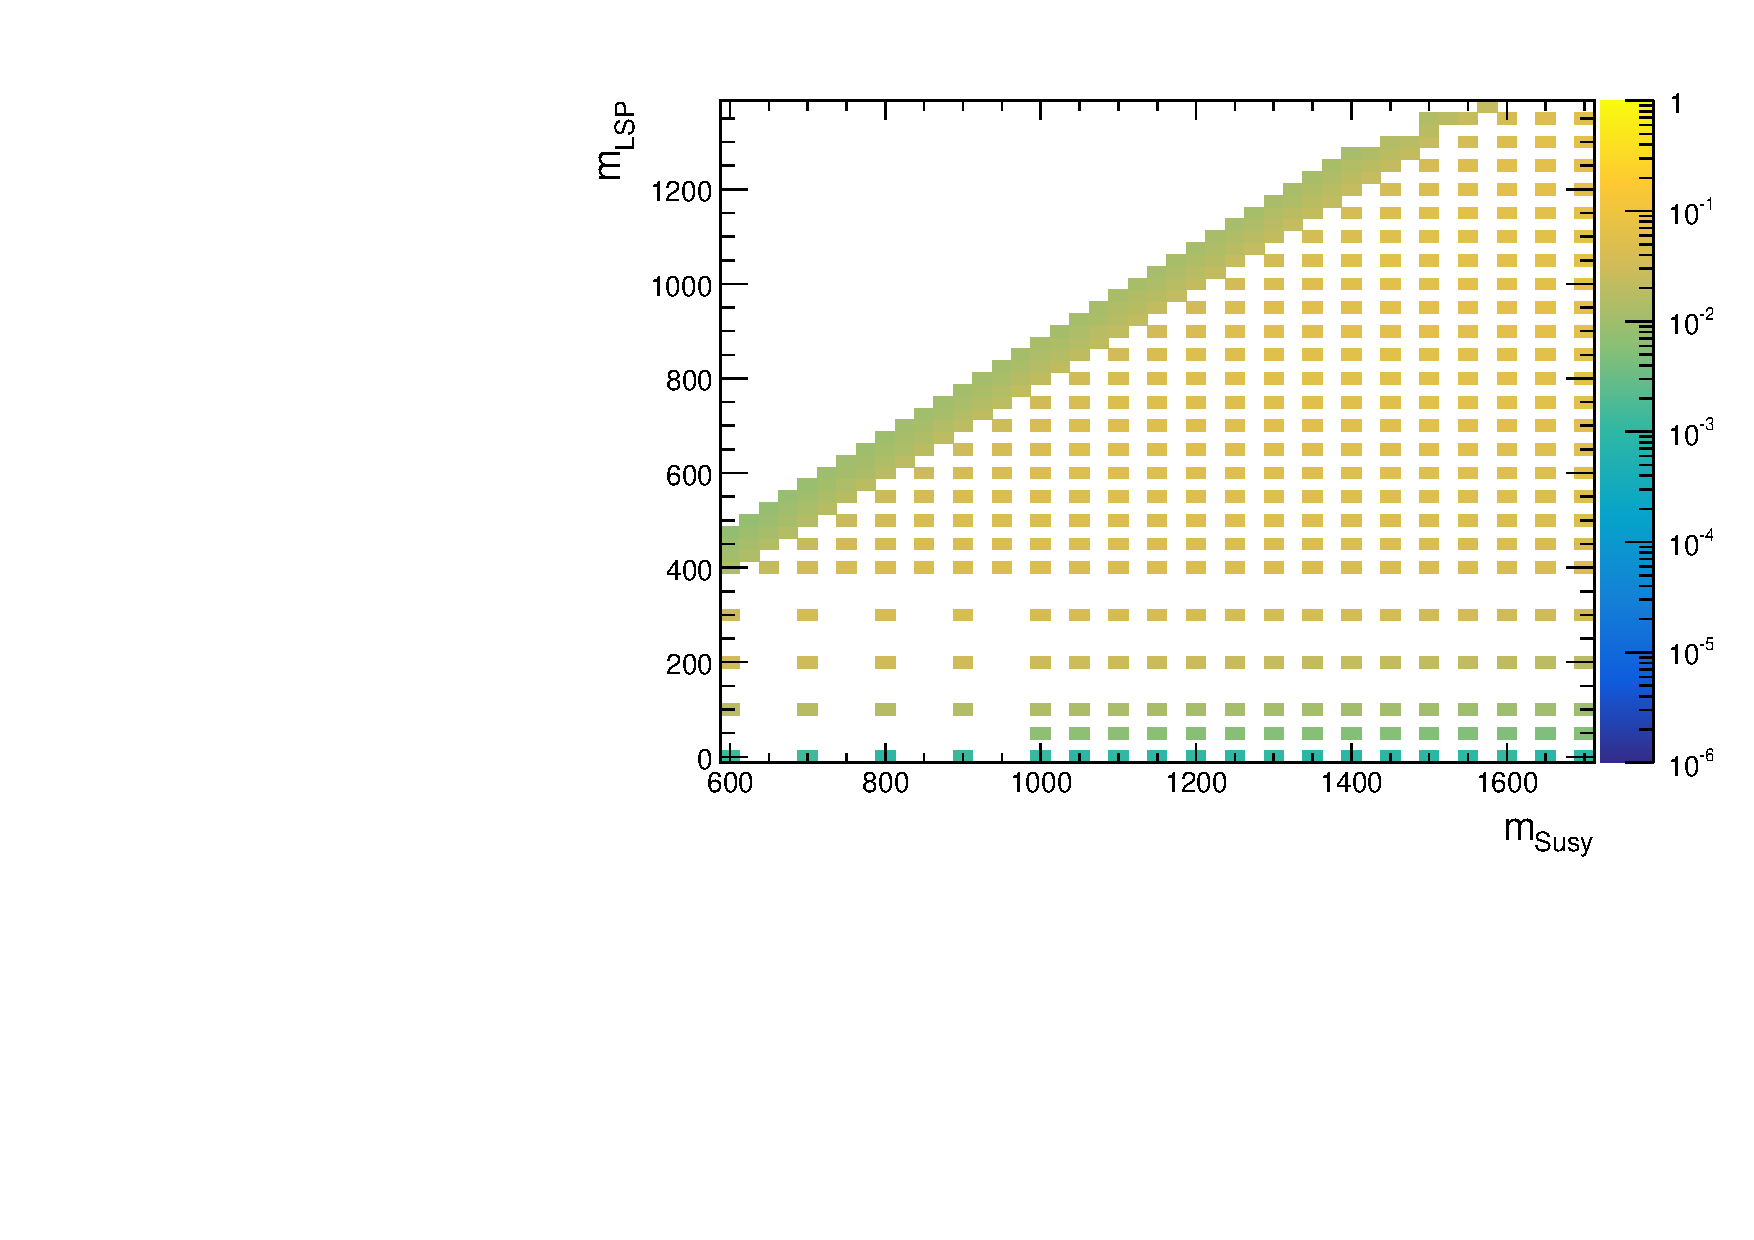
\includegraphics[width=0.49\textwidth]{supplementary/figures/T5tttt_degen_merging_4_cats} \,     
  \end{center}
  \caption{Left: (coloured histogram) upper limit on the cross section in the $(m_{\mathrm{Gluino}},m_{\mathrm{LSP}})$ plane for the T5tttt\_degen model. 
  The black (red) solid line is the observed (expected) exclusion. The red dashed lines are the $\pm1\sigma$ expected exclusion due to experimental uncertainties. 
  The $\pm1\sigma$ observed exclusion due to theoretical uncertainties on the signal cross section are shown as thin black lines. 
  Right: signal efficiency for the search regions included in the limit calculation as a function $(m_{\mathrm{Gluino}},m_{\mathrm{LSP}})$ plane for the T5tttt\_degen model. 
  \label{fig:T5tttt_degen_excl}}
\end{figure*}

\begin{figure*}[t]
  \begin{center}
    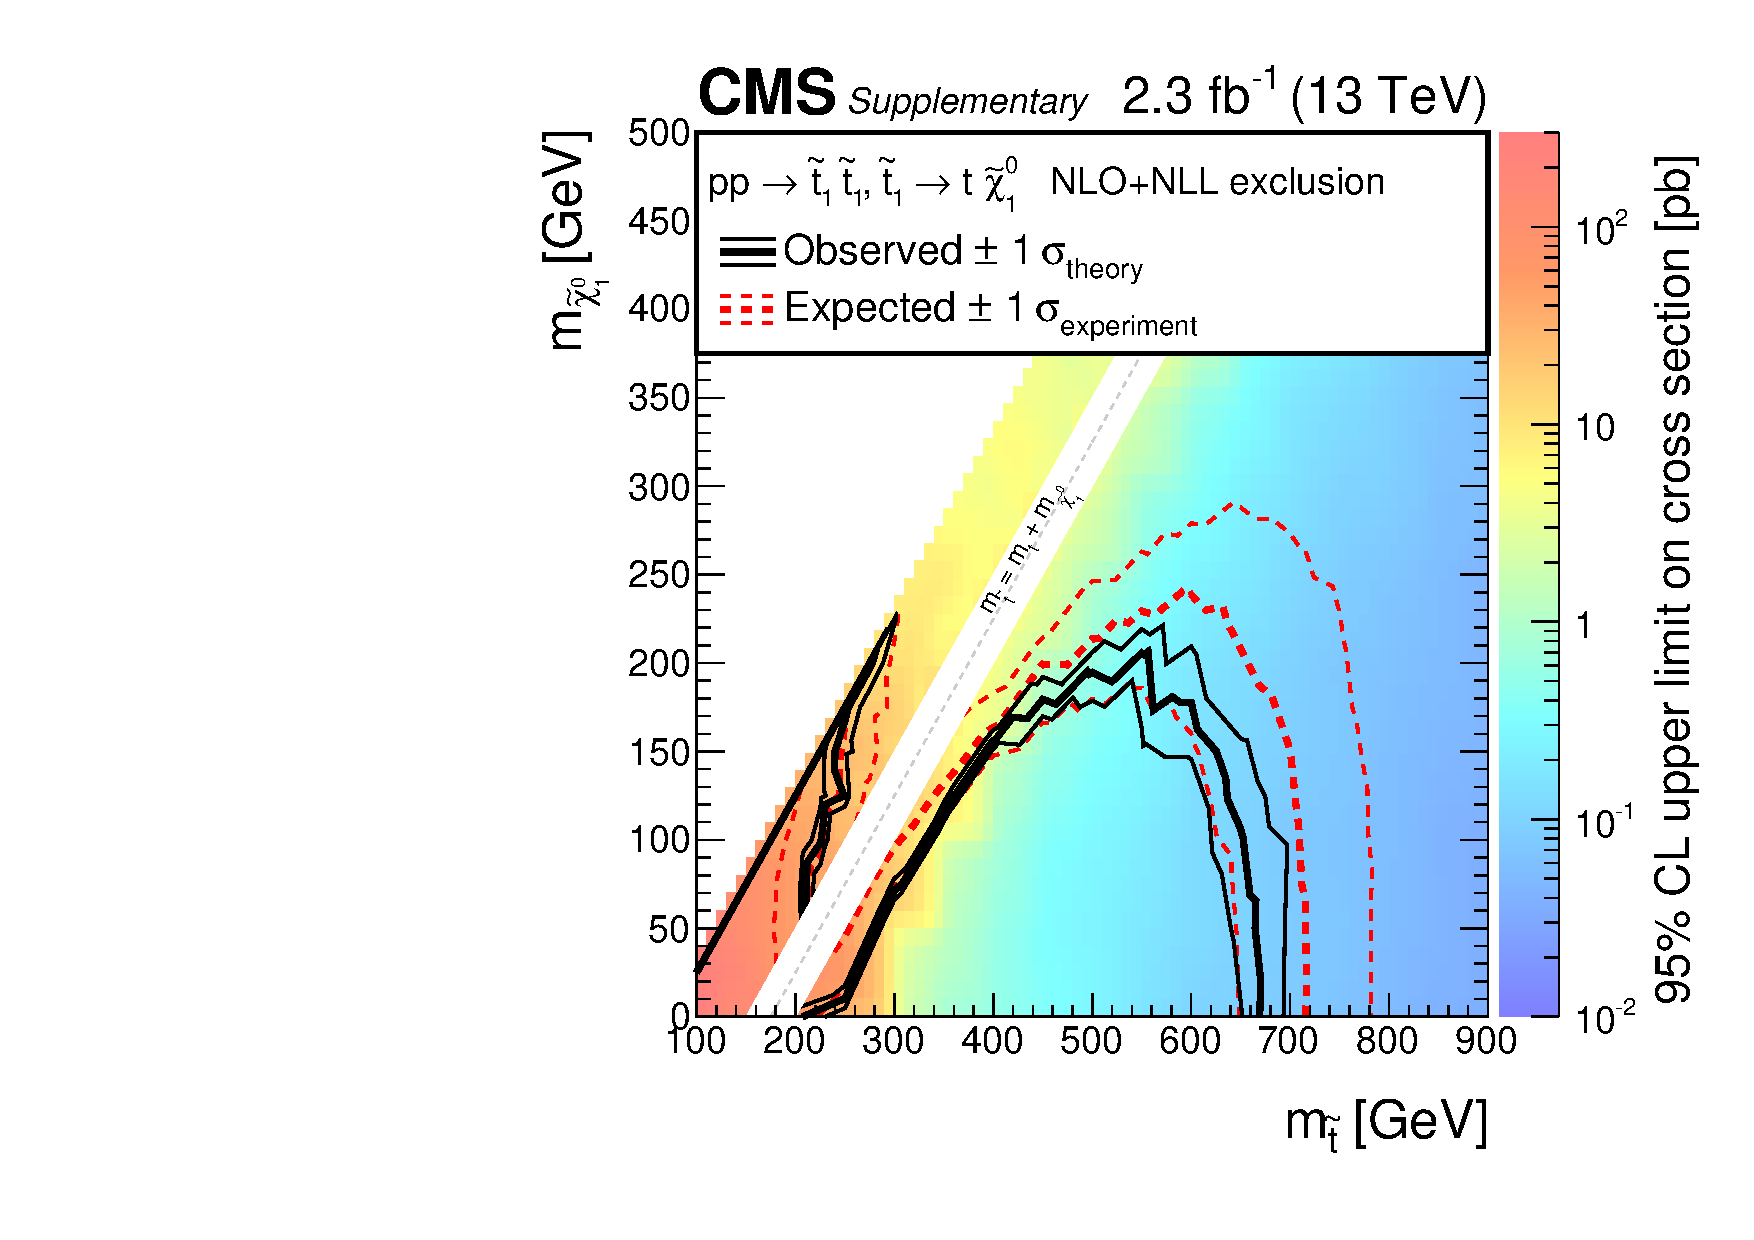
\includegraphics[width=0.49\textwidth]{supplementary/figures/RA1T2ttXSEC} \, 
    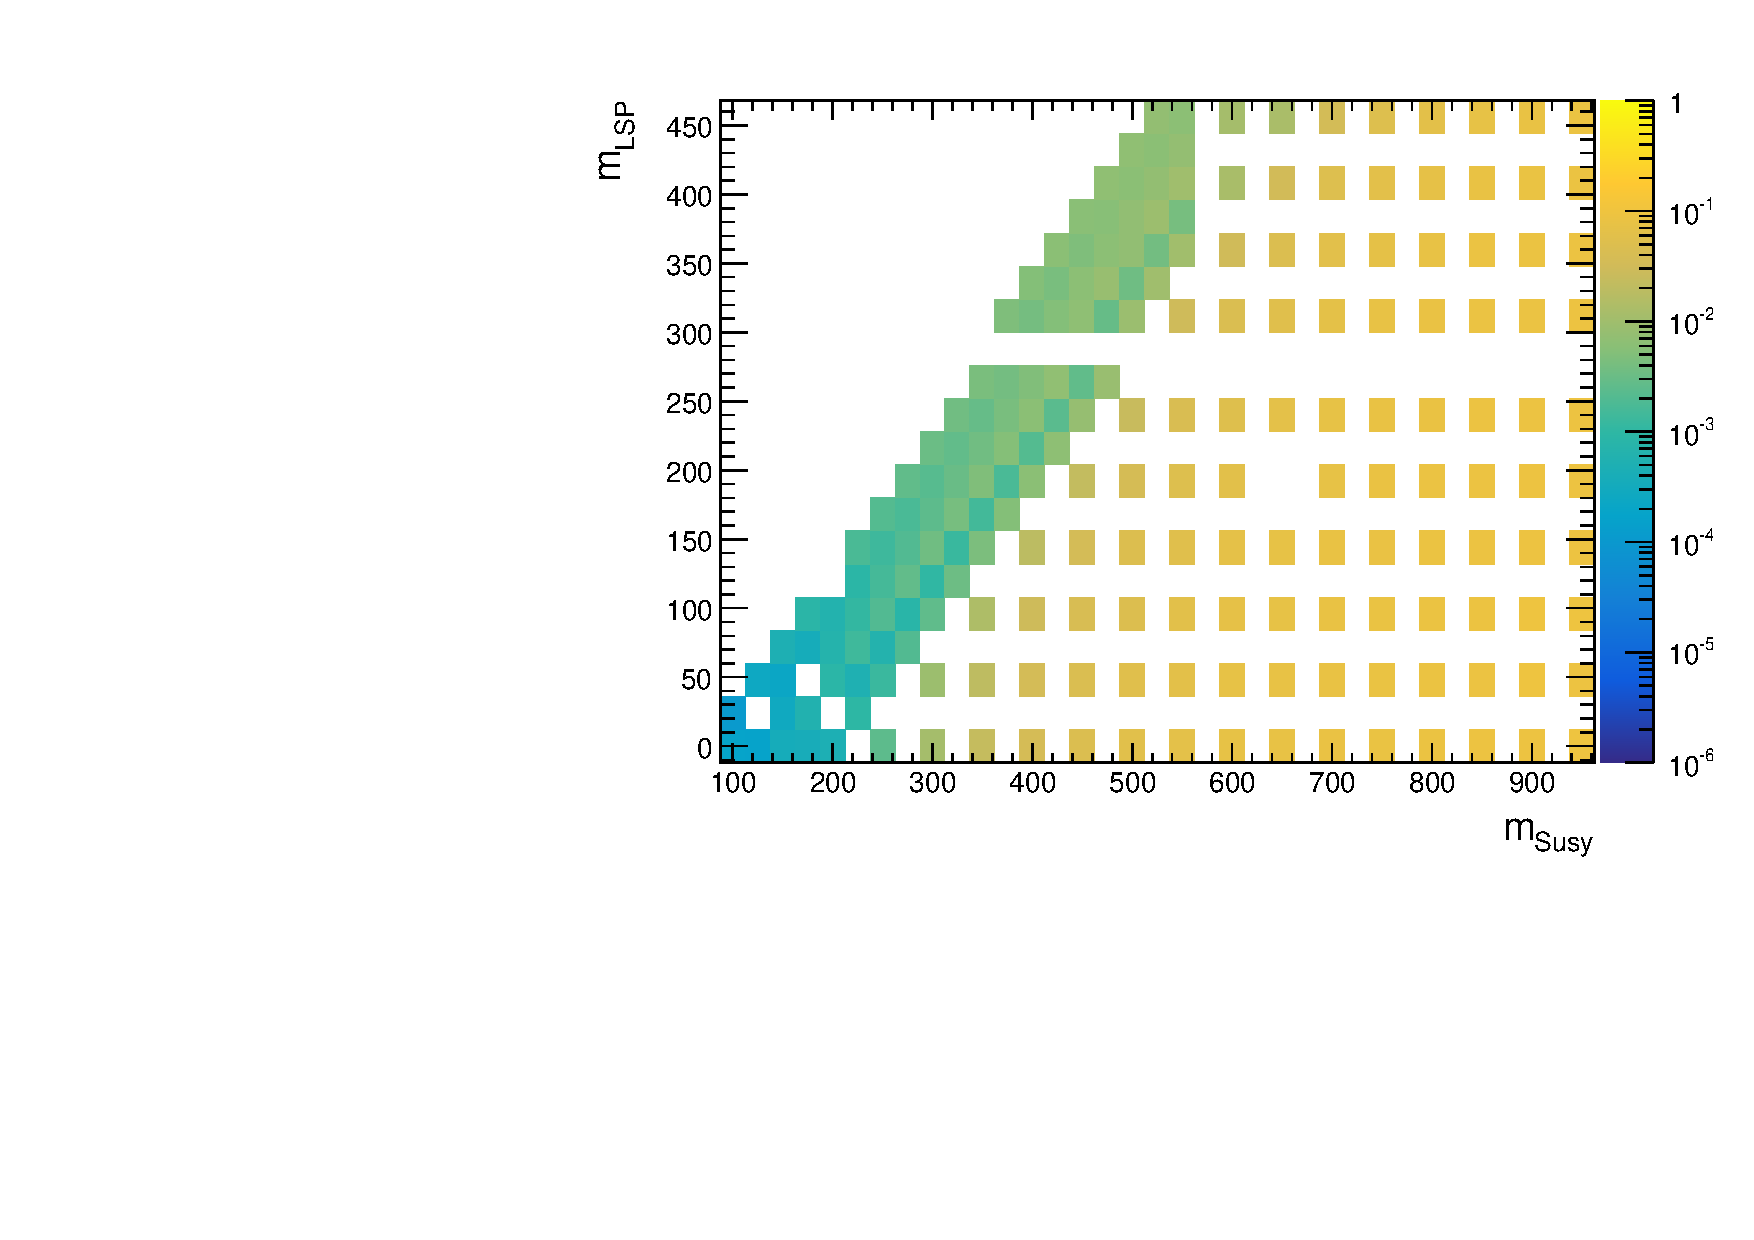
\includegraphics[width=0.49\textwidth]{supplementary/figures/T2tt_merging_4_cats} \,     
  \end{center}
  \caption{Left: (coloured histogram) upper limit on the cross section in the $(m_{\mathrm{Gluino}},m_{\mathrm{LSP}})$ plane for the T2tt model. 
  The black (red) solid line is the observed (expected) exclusion. The red dashed lines are the $\pm1\sigma$ expected exclusion due to experimental uncertainties. 
  The $\pm1\sigma$ observed exclusion due to theoretical uncertainties on the signal cross section are shown as thin black lines. 
  Right: signal efficiency for the search regions included in the limit calculation as a function $(m_{\mathrm{Gluino}},m_{\mathrm{LSP}})$ plane for the T2tt model. 
  \label{fig:T2tt_excl}}
\end{figure*}


\clearpage
\begin{figure*}[t]
  \begin{center}
    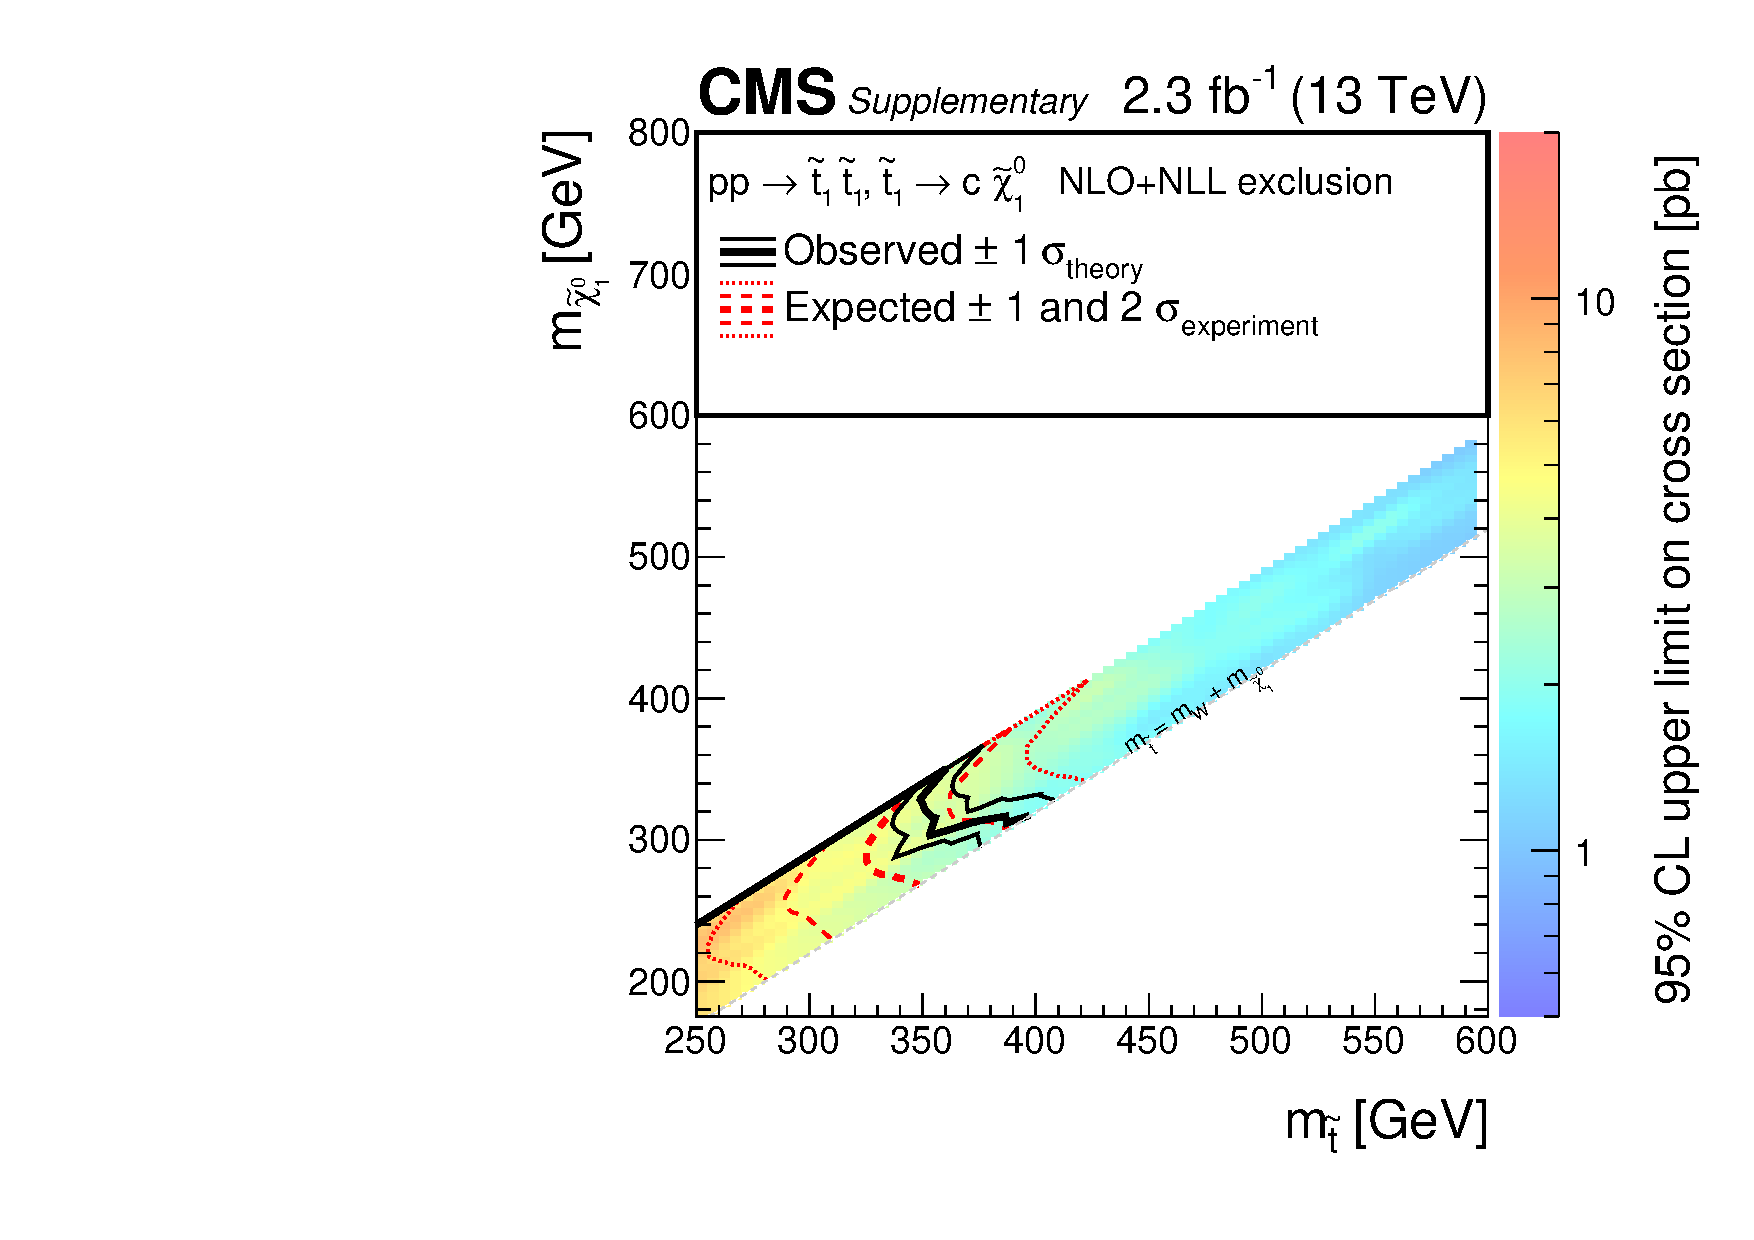
\includegraphics[width=0.49\textwidth]{supplementary/figures/RA1T2ccXSEC} \, 
    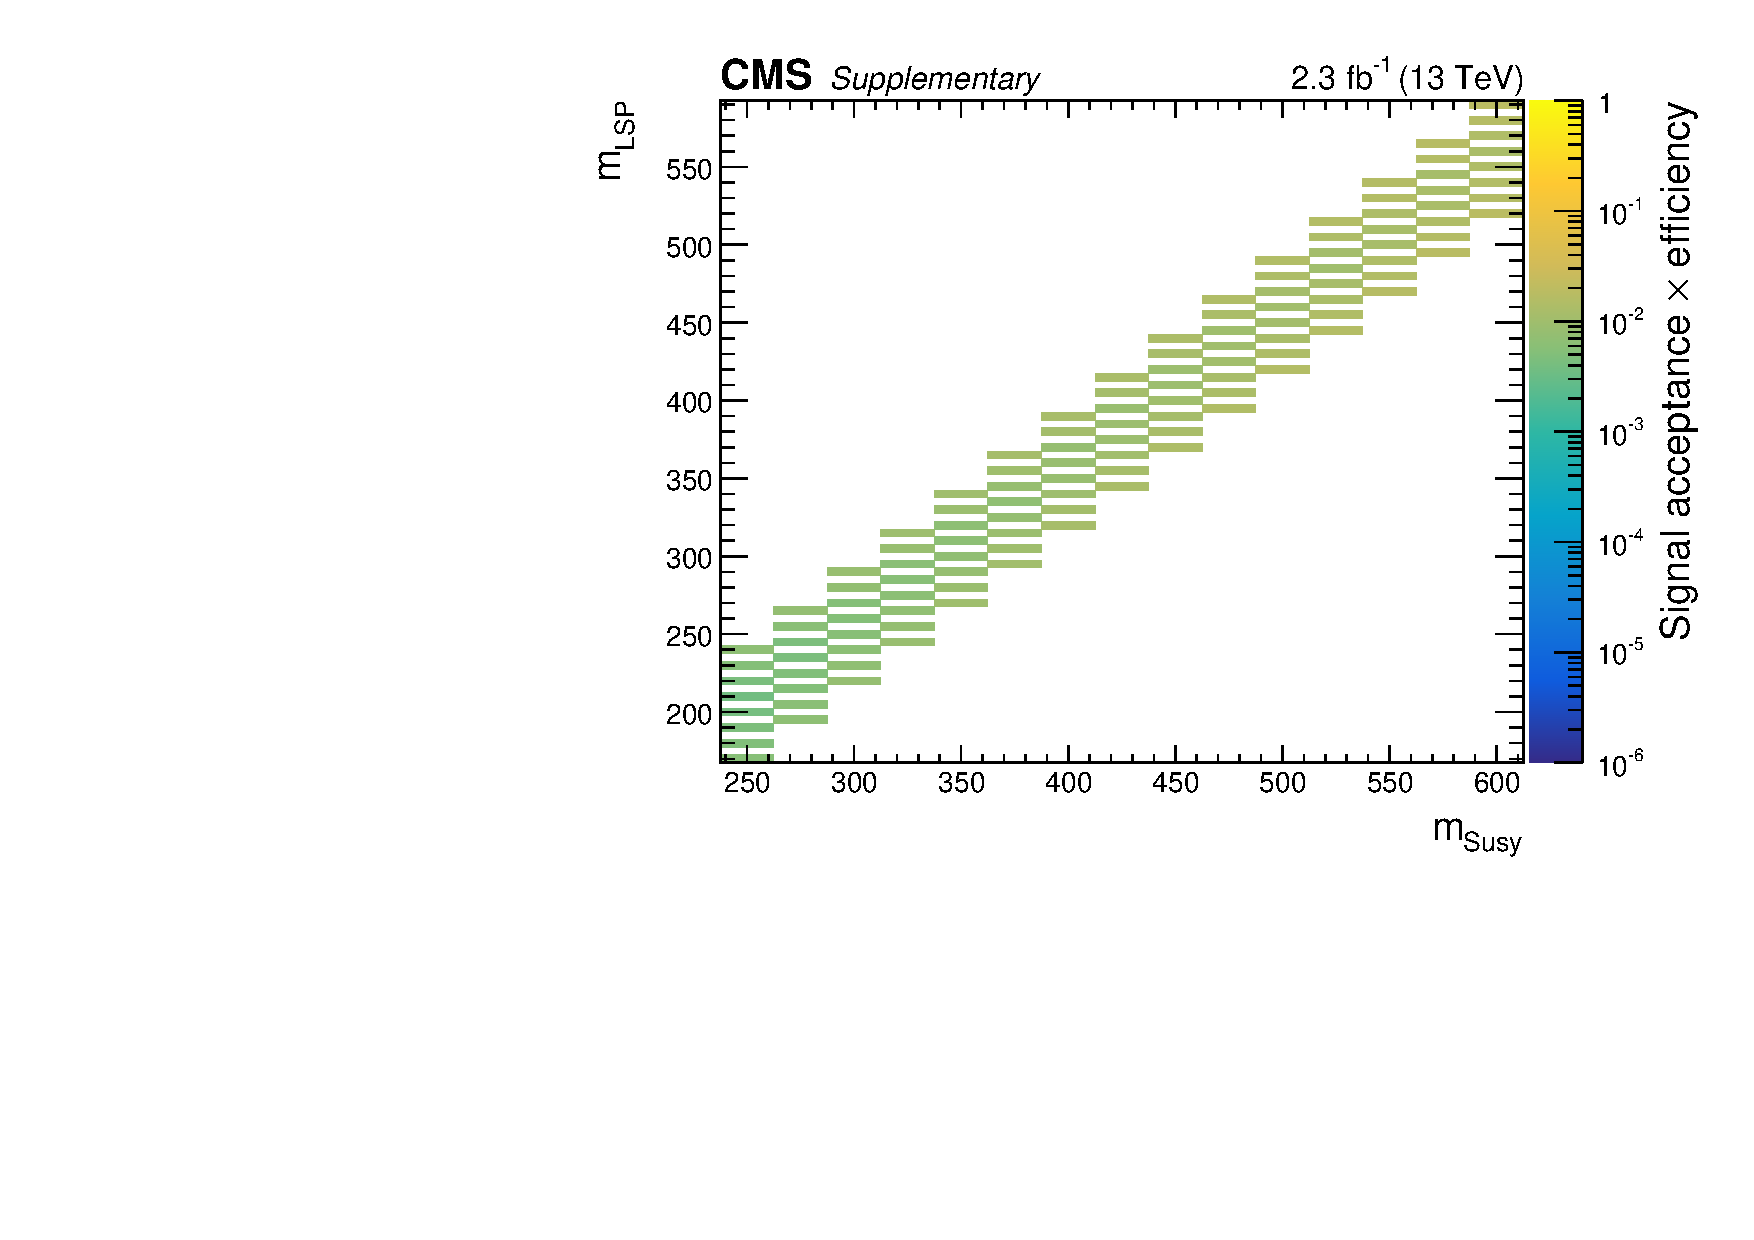
\includegraphics[width=0.49\textwidth]{supplementary/figures/T2cc_merging_4_cats} \,     
  \end{center}
  \caption{Left: (coloured histogram) upper limit on the cross section in the $(m_{\mathrm{Gluino}},m_{\mathrm{LSP}})$ plane for the T2cc model. 
  The black (red) solid line is the observed (expected) exclusion. The red dashed lines are the $\pm1\sigma$ expected exclusion due to experimental uncertainties. 
  The $\pm1\sigma$ observed exclusion due to theoretical uncertainties on the signal cross section are shown as thin black lines. 
  Right: signal efficiency for the search regions included in the limit calculation as a function $(m_{\mathrm{Gluino}},m_{\mathrm{LSP}})$ plane for the T2cc model. 
  \label{fig:T2cc_excl}}
\end{figure*}

\begin{figure*}[t]
  \begin{center}
    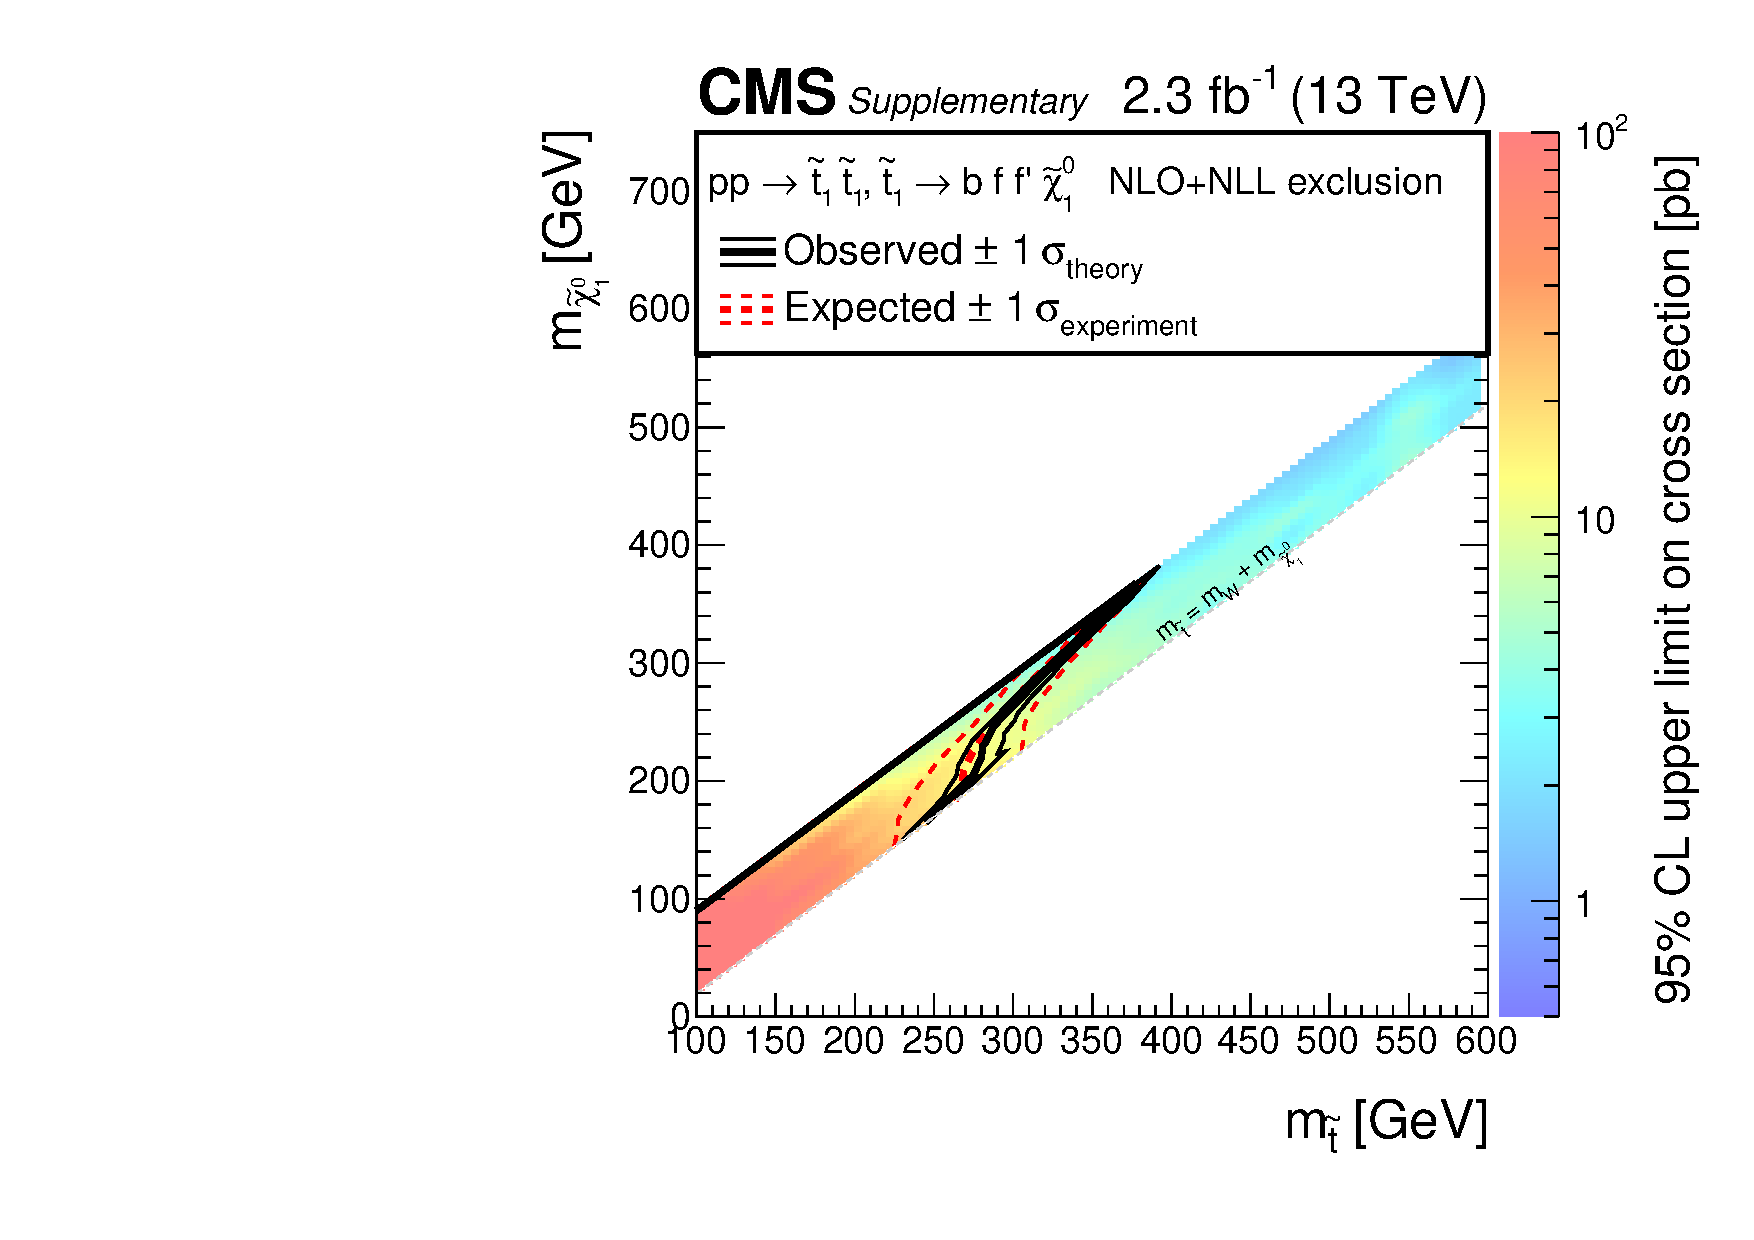
\includegraphics[width=0.49\textwidth]{supplementary/figures/RA1T2-4bdXSEC} \, 
    \includegraphics[width=0.49\textwidth]{supplementary/figures/T2-4bd_merging_4_cats} \,     
  \end{center}
  \caption{Left: (coloured histogram) upper limit on the cross section in the $(m_{\mathrm{Gluino}},m_{\mathrm{LSP}})$ plane for the T2-4bd model. 
  The black (red) solid line is the observed (expected) exclusion. The red dashed lines are the $\pm1\sigma$ expected exclusion due to experimental uncertainties. 
  The $\pm1\sigma$ observed exclusion due to theoretical uncertainties on the signal cross section are shown as thin black lines. 
  Right: signal efficiency for the search regions included in the limit calculation as a function $(m_{\mathrm{Gluino}},m_{\mathrm{LSP}})$ plane for the T2-4bd model. 
  \label{fig:T2-4bd_excl}}
\end{figure*}


\clearpage
\begin{figure*}[t]
  \begin{center}
    \includegraphics[width=0.49\textwidth]{supplementary/figures/RA1T2mixedXSEC} \, 
    \includegraphics[width=0.49\textwidth]{supplementary/figures/T2mixed_merging_4_cats} \,     
  \end{center}
  \caption{Left: (coloured histogram) upper limit on the cross section in the $(m_{\mathrm{Gluino}},m_{\mathrm{LSP}})$ plane for the T2mixed model. 
  The black (red) solid line is the observed (expected) exclusion. The red dashed lines are the $\pm1\sigma$ expected exclusion due to experimental uncertainties. 
  The $\pm1\sigma$ observed exclusion due to theoretical uncertainties on the signal cross section are shown as thin black lines. 
  Right: signal efficiency for the search regions included in the limit calculation as a function $(m_{\mathrm{Gluino}},m_{\mathrm{LSP}})$ plane for the T2mixed model. 
  \label{fig:T2mixed_excl}}
\end{figure*}

\begin{figure*}[t]
  \begin{center}
    \includegraphics[width=0.49\textwidth]{supplementary/figures/RA1T2tbXSEC} \, 
    \includegraphics[width=0.49\textwidth]{supplementary/figures/T2tb_merging_4_cats} \,     
  \end{center}
  \caption{Left: (coloured histogram) upper limit on the cross section in the $(m_{\mathrm{Gluino}},m_{\mathrm{LSP}})$ plane for the T2tb model. 
  The black (red) solid line is the observed (expected) exclusion. The red dashed lines are the $\pm1\sigma$ expected exclusion due to experimental uncertainties. 
  The $\pm1\sigma$ observed exclusion due to theoretical uncertainties on the signal cross section are shown as thin black lines. 
  Right: signal efficiency for the search regions included in the limit calculation as a function $(m_{\mathrm{Gluino}},m_{\mathrm{LSP}})$ plane for the T2tb model. 
  \label{fig:T2tb_excl}}
\end{figure*}


\clearpage
\begin{figure*}[t]
  \begin{center}
    \includegraphics[width=0.49\textwidth]{supplementary/figures/RA1T2bW-X05XSEC} \, 
    \includegraphics[width=0.49\textwidth]{supplementary/figures/T2bW_X05_merging_4_cats} \,     
  \end{center}
  \caption{Left: (coloured histogram) upper limit on the cross section in the $(m_{\mathrm{Gluino}},m_{\mathrm{LSP}})$ plane for the T2bW\_X05 model. 
  The black (red) solid line is the observed (expected) exclusion. The red dashed lines are the $\pm1\sigma$ expected exclusion due to experimental uncertainties. 
  The $\pm1\sigma$ observed exclusion due to theoretical uncertainties on the signal cross section are shown as thin black lines. 
  Right: signal efficiency for the search regions included in the limit calculation as a function $(m_{\mathrm{Gluino}},m_{\mathrm{LSP}})$ plane for the T2bW\_X05 model. 
  \label{fig:T2bW_X05_excl}}
\end{figure*}

\begin{figure*}[t]
  \begin{center}
    \includegraphics[width=0.49\textwidth]{supplementary/figures/RA1T2bbXSEC} \, 
    \includegraphics[width=0.49\textwidth]{supplementary/figures/T2bb_merging_4_cats} \,     
  \end{center}
  \caption{Left: (coloured histogram) upper limit on the cross section in the $(m_{\mathrm{Gluino}},m_{\mathrm{LSP}})$ plane for the T2bb model. 
  The black (red) solid line is the observed (expected) exclusion. The red dashed lines are the $\pm1\sigma$ expected exclusion due to experimental uncertainties. 
  The $\pm1\sigma$ observed exclusion due to theoretical uncertainties on the signal cross section are shown as thin black lines. 
  Right: signal efficiency for the search regions included in the limit calculation as a function $(m_{\mathrm{Gluino}},m_{\mathrm{LSP}})$ plane for the T2bb model. 
  \label{fig:T2bb_excl}}
\end{figure*}


\clearpage
\begin{figure*}[t]
  \begin{center}
    \includegraphics[width=0.49\textwidth]{supplementary/figures/RA1T2qqXSEC} \, 
    \includegraphics[width=0.49\textwidth]{supplementary/figures/T2qq_merging_4_cats} \,     
  \end{center}
  \caption{Left: (coloured histogram) upper limit on the cross section in the $(m_{\mathrm{Gluino}},m_{\mathrm{LSP}})$ plane for the T2qq model. 
  The black (red) solid line is the observed (expected) exclusion. The red dashed lines are the $\pm1\sigma$ expected exclusion due to experimental uncertainties. 
  The $\pm1\sigma$ observed exclusion due to theoretical uncertainties on the signal cross section are shown as thin black lines. 
  Right: signal efficiency for the search regions included in the limit calculation as a function $(m_{\mathrm{Gluino}},m_{\mathrm{LSP}})$ plane for the T2qq model. 
  \label{fig:T2qq_excl}}
\end{figure*}




\clearpage
\begin{figure*}[thp!]
  \begin{center}
    \includegraphics[width=0.49\textwidth]{figures/mixSUMMARY_transposed.pdf}
    \includegraphics[width=0.49\textwidth]{figures/gluinoSUMMARY_transposed.pdf} \\
    \includegraphics[width=0.49\textwidth]{figures/naturalSUMMARY_transposed.pdf}
    \includegraphics[width=0.49\textwidth]{figures/allThirdGenSUMMARY_transposed.pdf} \\
    \caption{Summary for the observed (solid lines) and expected (dashed lines) exclusions in the $m_{\mathrm{Susy}},m_{\mathrm{Susy}}-m_{\mathrm{LSP}}$ plane for the models considered in the analysis. 
       Exclusion contours are grouped into 4 summary plots: 
       ``Direct and gluino-mediated production of off-shell (decoupled) light-flavour squarks'' (top left), ``Gluino-mediated production of off-shell (decoupled) 3rd generation squarks'' (top right), ``Gluino-mediated production of on-shell stops and charginos (natural models)'' (bottom left), ``Direct production of 3rd generation squarks'' (bottom right). 
      \label{fig:summary-excl-plots} }
  \end{center}
\end{figure*}



\clearpage
% \nocite{*}
\bibliography{auto_generated}
